\documentclass[12pt]{article}
\usepackage{graphicx}
\topmargin -1in
\textwidth 6.5in
\textheight 9.5 in
\oddsidemargin 0.0in
\evensidemargin 0.0in
\baselineskip 14pt
\makeindex
\def\see#1#2{{\em see\/} #1}
\begin{document}
\begin{flushright}
\vspace*{0.5in}
CDF Note: CDF/DOC/COMP\_UPG/PUBLIC/3891 \\
\index{CDF}
D0 Note: 3118f \\
\index{D0}
Computing Division Note: GU0013 \\
\end{flushright}
\vspace{0.5in}
\begin{center}
{\LARGE SoftRelTools User's Guide}\\
\vspace{.5in}
{\large Version 2.0}\\
{\large \today }\\
\vspace{.5in}
{\large Last edited by Margaret Votava}\\
{\large \em Fermilab Computing Division}\\
\vspace{.5in}
{\large for:\\
Dave Adams, Jim Amundson, Jim Bellinger, Walter Brown, Glenn Cooper, 
Flavia Donno-Raffaelli, Lynn Garren, 
Herb Greenlee, Robert Harris, Alan Jonckheere, Robert Kennedy, Arthur Kreymer, 
Qizhong Li, Don Petravick, Ruth Pordes, Lars Rasmussen, 
Elizabeth Sexton-Kennedy, Scott Snyder and Gordon Watts.}
\vspace{.5in}
\end{center}
\begin{abstract}
This is the user's guide for the Fermilab version of Software Release Tools, 
a UNIX based software management system for large, collaborative projects
that is used by several experiments at Fermilab.
The system provides software version control with CVS\index{CVS} 
configured in a client-server\index{client-server} mode.
For management and 
building we have adopted the directory structure and SoftRelTools originally 
developed by the BaBar collaboration. 
The system handles the 
version control, management, building, and distribution of code written in 
Fortran, C and C++. A distinguishing feature of the system is its
\index{C++}
ability to allow rapid asynchronous development of 
package versions, 
which can be easily integrated into complete consistent
releases\index{releases} of the entire offline software.  This 
has reduced the time it takes for new and modified code to be made available to 
users. 
\end{abstract}

\clearpage
\tableofcontents
\listoffigures
\listoftables

\clearpage
\section{Introduction}

This document is the User's Guide for SoftRelTools (SRT). It is meant
to give an overview of the SRT environment and commands
from a code developers point
of view. Code librarians should refer to the SRT Reference Guide for
more detailed explanation of the SRT configuration parameters and commands. 

SRT is very flexible in the style in which it allows developers to operate. 
This flexibility presents a difficulty in writing a general purpose "how to"
User's Guide because each librarian has imposed a cycle that is most 
appropriate for that particular release and a naming convention that
best suits the cycle. Users should refer to the specific instructions 
for a given release for the naming conventions and the development cycle. 

Release specific instructions can be found at:
\begin{itemize}
\item CDF Run 2
\item D0 Run 2
\item SDSS
\item ZOOM
\item BTeV http://www-btev.fnal.gov/internal\_documents/code/code\_management.html
\item Minos 
\end{itemize}

\subsection{What is SRT}

SoftRelTools (SRT) is a toolset for managing large software projects, aka releases,
that consists of smaller units, aka packages, that are developed in parallel
by a diverse programming community. It allows individual developers to 
work on their package independently of the ongoing work in other packages,
and to update the whole project when they are satisfied with their 
modifications. In this way, the developer is responsible for the management
of his individual package, while the release librarian is responsible for 
management of the all the packages as a whole.


\subsection{How to use this document}
This document has been written in the style of a book, or pedagogical users
manual, with discussion and illustrations.  People seeking a general 
overview of the system may want to read the normal sections, omitting the 
appendices.  New users or developers who want to do something with the system 
quickly, and don't want to read much, are advised to follow the examples in 
section~\ref{sec_examples} and Appendix~\ref{app_build}. Those seeking a 
reference manual for answering arbitrary questions about the system will find
it quickest to use the index at the back of the document.  

\subsection{Other light reading}

For sleepless nights:
\begin{itemize}
\item SRT Reference Guide
\item CVS User's Guide http://www.fnal.gov/docs/products/cvs/
\item gmake User's Guide http://www.fnal.gov/docs/products/gtools/make.1.html
\item Barbar SRT document
\item CVSH http://www.fnal.gov/cd/FUE/cvsh/ 
\end{itemize}

\section{Software Release Structure}
The software release structure provides a flexible and easy to use
framework for both releasing and developing code.  Code is typically grouped
into {\em packages}\index{packages!definition}; however, it is essential to have a {\em release} of all 
code in 
all packages. The structure must support simultaneously both
releases\index{releases} of stable versions of the 
packages\index{packages}, and asynchronous development of 
the individual packages themselves.  This is in contrast to a structure which
is oriented solely along the lines of a release, where package versions
are only stamped with the release number. The BaBar software release
\index{BaBar}
structure~\cite{ref_babar1,ref_babar2}, which supports both
asynchronous development of packages\index{packages!asynchronous development} 
and grouping packages\index{packages} into 
releases\index{releases!definition},
is shown in Fig.~\ref{fig_directory}. A commentary on this structure with 
a detailed verbal description of Fig.~\ref{fig_directory} is given in 
Appendix~\ref{app_commentary}.

The environmental variable {\ttfamily \$SRT\_DIST} is used as a root to add flexibility.  
Below it are found separate subtrees for packages\index{packages} and releases\index{releases}. 
Within the
package subtree, each package can contain one or more different {\em versions}.
This allows the package librarians to develop packages 
asynchronously\index{packages!asynchronous development},
and assign the package a version number when the package is ready for use
by others.  Within the release subtree, there is a subdirectory for each
existing release.  A release directory consists of soft links to a set of 
\index{soft links}
consistent package versions, plus the libraries and binaries created from
the release for various machine architectures.  Again, the release manager
can use this to create releases\index{releases} as required.  Links within the release
\index{soft links}
directory can be used to provide default names for particular releases, for
example ``current'' for the release recommended for general use at the present
time.

Notice that the soft links between releases\index{releases!soft links} and 
packages\index{packages!soft links} are
\index{soft links}
to the source code only; the libraries and binaries are native to the release.
This is necessary because in C++ a change to a header file used by package A can
\index{C++}
affect the result in package B which uses package A, even if package B does 
not use the part of the header file that is changed or added.  Unlike common
blocks in Fortran, where you can add to the end of a common block which is
used by many packages\index{packages} and you do not need to recompile all the code, in C++
\index{compile}
\index{C++}
if you modify a header file you have to recompile all the code that depends on 
\index{dependencies!and C++} 
that header file. The only way to insure consistent results when
changing a header file is to rebuild both libraries.  

\begin{figure}[tbh]
%\centerline{\epsfig{figure=run_2_directory.eps,width=4.5in}}
\begin{center}
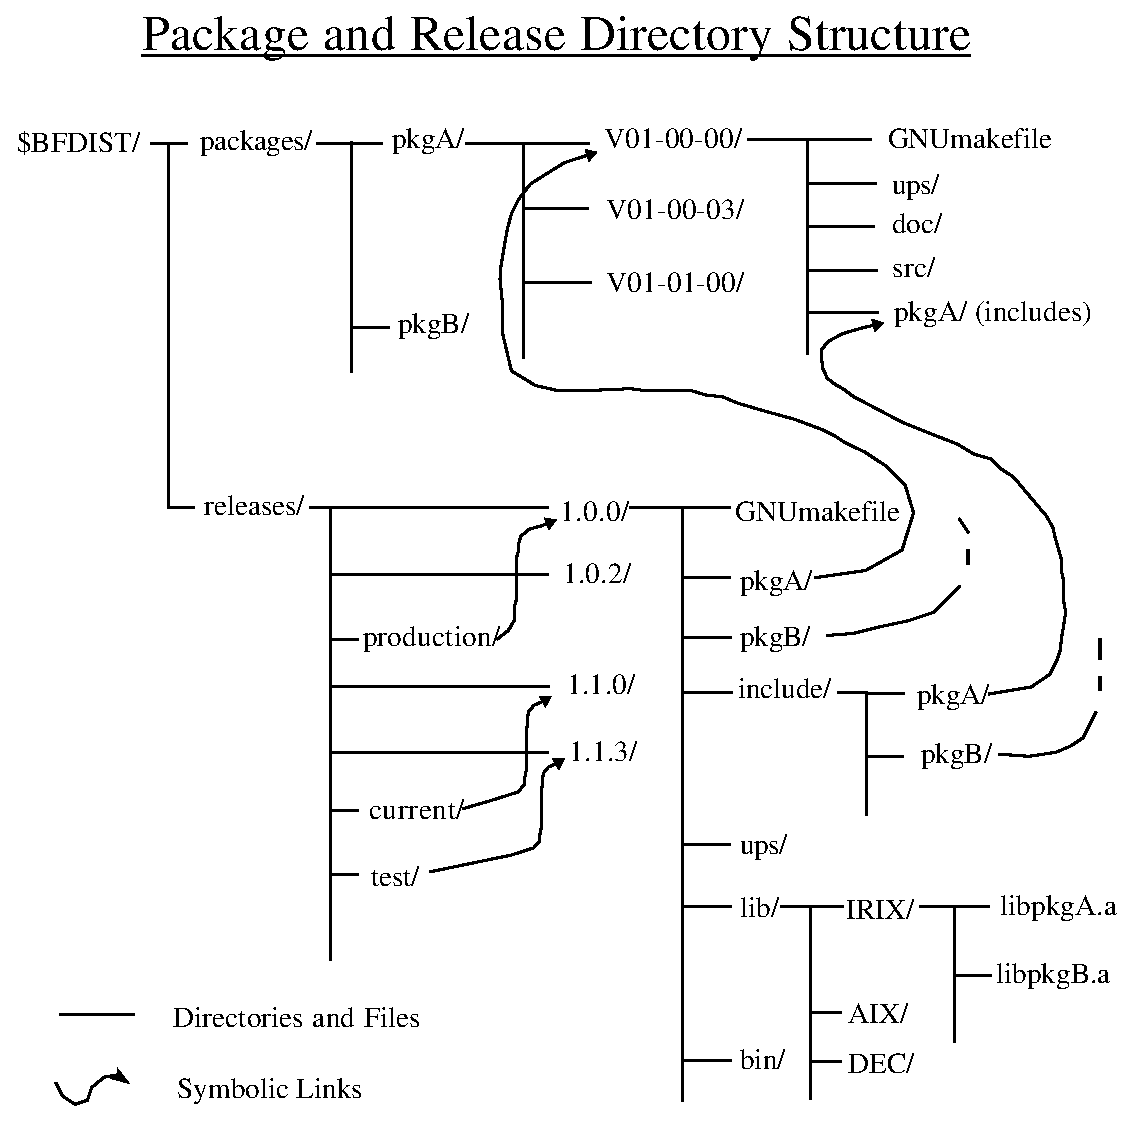
\includegraphics[width=4.5in]{run_2_directory.eps}
\end{center}
\caption[Official Release Directory Structure]{ 
Diagram of the directory structure.  This example includes two
packages: 
``pkgA'' and ``pkgB''\index{packages!definition}\index{packages!figure}. 
The curved lines correspond to soft links\index{soft links} between 
releases\index{releases!definition}\index{releases!figure} and packages.}
\label{fig_directory}
\end{figure}

\subsection{Package and Release Versions and Labels}
\index{version!of package}
\index{version!numbering convention}
The package and release numbering system is designed to allow multiple versions
of packages\index{packages!numbering} and many releases\index{releases!numbering} of code to be available to the collaboration.

The convention for package version numbers is Vxx-yy-zz where
xx is the major version field, yy the minor field, and zz is a bug fix
field incremented for small changes. This version number is also the 
CVS\index{CVS!tag or version} tag of 
that version. The first version is then V00-00-00.
The code manager will install this tag on the initial version of
the code in the repository, and either librarians or the code manager can tag 
subsequent versions using the CVS\index{CVS!commands!rtag} command rtag.

The convention for releases\index{releases!numbering} is x.y.z, where x is the 
major release number\index{releases!major},
y the minor release\index{releases!major}, and z is a bug fix 
number\index{releases!bug-fix}. Thus 1.0.0 would be a major
release that is rigorously tested,  1.1.0 would be a minor release based on 
1.0.0 and would require less testing, and 1.1.3 would be a bug fix or fast 
release based on 1.1.0 and might have almost no testing.  The ``production''
release would generally be a symbolic link to a major release, like 1.0.0.
\index{soft links}
The ``current'' release could be a minor release, like 1.1.0. The ``test'' release 
could be bug fix release, such as 1.1.3.  There could be many major, minor,
and bug fix releases\index{releases!bug-fix}, and only a few of them might have symbolic links pointing
\index{soft links}
to them with names like ``production'', ``current'', ``test'',
``fast-tracking'', etc.
This labelling system allows many different releases, and the level of
validation\index{releases!validation} is apparent from the number.

\subsection{Development Releases}
\label{sec_development}

\index{development} 
In addition to frozen releases with specific versions, SRT structure
also supports a more dynamic development environment. A development release is 
not required, but it is a very useful option for integration, bug detection,
and access to the most recent available code. Most often, 
developers are making changes on different packages in parallel. At
various stages during this development, they will want to share there
work with others. Making a frozen release for each of these stages
would consume a lot of disk space in addition to being a code librarian's
nightmare. 

In Fig.~\ref{fig_development_release} we show the structure of a development
release, which is nearly identical to a frozen release.  The difference is that
the soft links all point to the ``development'' version of the package in the
packages area.  The development version of the package was checked out of
CVS when the package was first added to development, and every day the 
development version is updated via a {\ttfamily cvs update} command. The 
{\ttfamily cvs update} command is a convenient way of distributing 
development, sending only the code that has changed from the repository to the 
development release.  Since we use client-server cvs, all nodes in the system 
are equal, and the process of getting development on a central system is no 
different than the process of getting development anywhere.  Note that no
development actually takes place in the development package area. Developers
are required to develop code in their test releases (see next section) and check
that code back in to the repository, so that the code can propogate to all
development nodes everywhere. 

\begin{figure}[tbh]
%\hspace*{0.1in}
%\epsfysize=6in
%\epsffile[36 100 581 674]{development_release.ps}
%\centerline{\epsfig{figure=development_release.eps,width=4.5in}}
\centerline{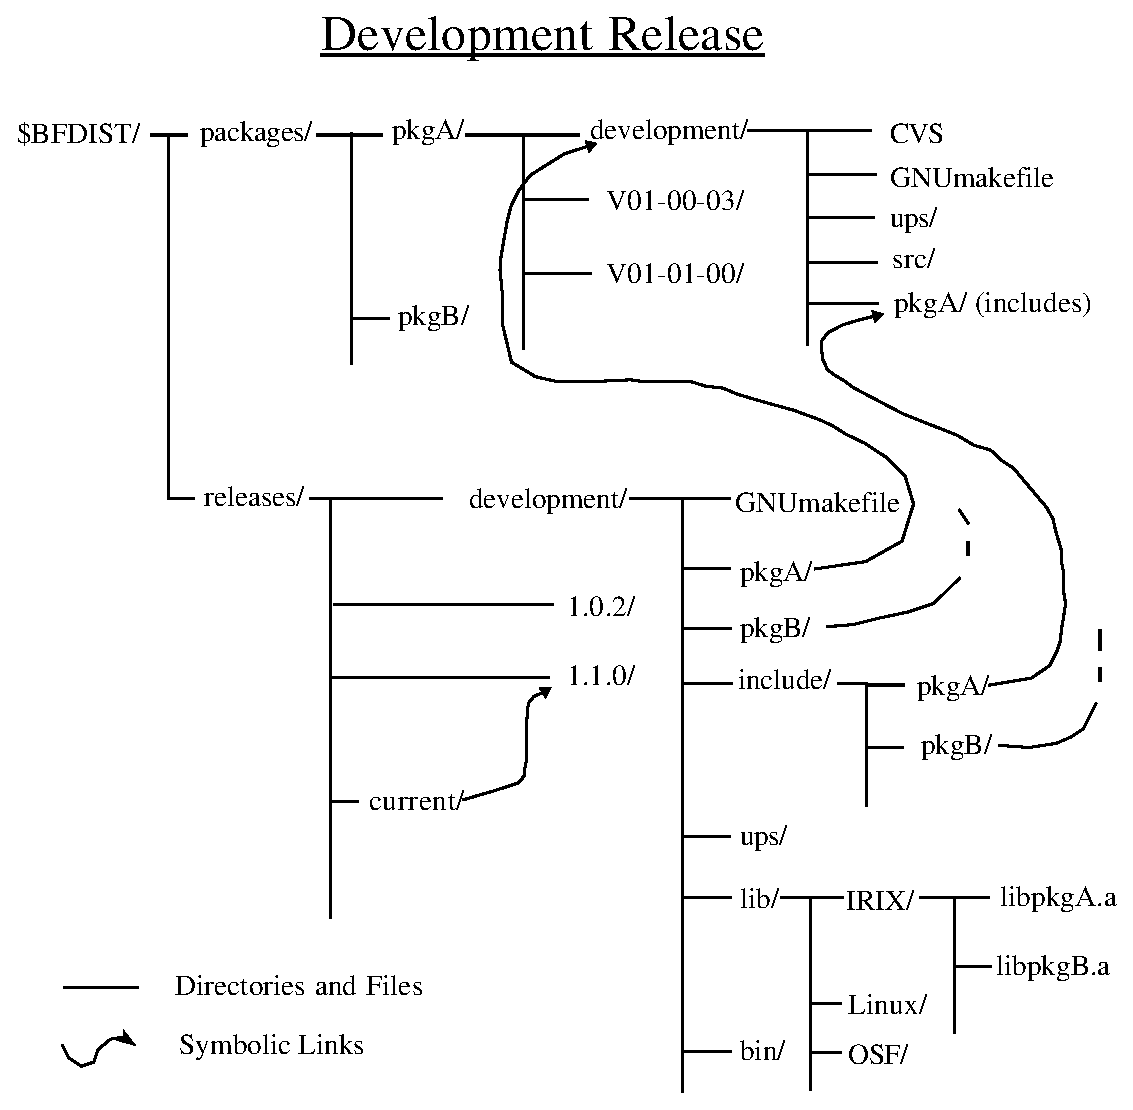
\includegraphics[width=4.5in]{development_release.eps}}
\vspace*{-0.5in}
\caption[Development Release Directory Structure]{ 
Same as Fig.~\ref{fig_directory} except the release called development
contains soft links to the development version of each package, which is 
checked out from CVS and updated from the main repository. There is nothing
hardwired about the tag "development", and each environment may have a 
different term. Please check the specific instructions from your code 
librarian.}
\label{fig_development_release}
\end{figure}

\index{development!update} 
At some interval on each development node 
{\ttfamily cvs update} is done for each package in the release, and 
then the release is rebuilt with the command {\ttfamily gmake}. At
CDF this happens every morning. Developers
can then use the development release to link against.  

A facility exists in 
SoftRelTools to scan the log files that result from the build,
find compilation and linking errors, and send error reports to the designated
developers and package librarians.  
\index{development!error reporting} 
This provides developers with immediate
feedback, and errors are caught and fixed quickly.  
This SoftRelTools error\_reporter facility
also can create error status tables, like the on in Fig.~\ref{fig_status_table}.
Ask your code librarian for links to the location of these log files. 

Although naive users may want to use a frozen release, for stability, 
in a rapidly developing software environment, developers need to use 
the development release to insure that their additions really work with
the most recent software.  

\begin{figure}[tbh]
%\centerline{\epsfig{figure=status_table.eps,width=4.5in}}
\centerline{\includegraphics[width=4.5in]{status_table.eps}}
\vspace*{-4.7in}
\caption[Status Table for Development Release]{ 
Example summary of errors detected during one night's build of the 
Run 2 development 
software at CDF. The lib stage is the compilation stage of the package,and 
the bin stage is the compilation and linking of executables for that package.
A text entry in the table indicates there was an error for the package 
indicated. Here for example there was an error linking an executable in the
TrackingMods package under Linux using the KAI compiler, and no errors 
anywhere else. This summary was generated on Wed Jul 22 08:00:19 1998 by the
error\_reporter facility in SoftRelTools.}
\label{fig_status_table}
\end{figure}

\subsection{Using the Software Release Structure}
\label{sec_examples}

This section will describe the overall procedures needed to develop
in an SRT environment.  In short, a user wants to develop a certain
package. He needs to define a context, or base release, in which this 
package will be compiled and linked. He must define a "test" release
in some working area, then copy the package to be modified
into this working area, and finally set symbolic links for header files
and libraries to the other packages in the base release - see Figure ???. 

The user is afforded many options to globally describe his development 
environment. One of which is a "super" test release. 
Look at figure ???. The default SRT behavior is to define
the path for header files to include both directories in the test 
release as well as the base release. If a user deleted a header file from 
package B in the test release, the make files would still find it in the
base release. This can lead to some confusion. SRT supports the concept
of a "super" test release which will only look for include files in the
test release. It does this by creating a directory called "super" in the
test release and putting links to each pacagke's header files therein. 


The SoftRelTools commands themselves are defined in more
detail in Section ~\ref{sec_commands}. 
Once again, you should
refer to your code librarian's instructions for the naming conventions and
practices unique to your specific configuration. Section~\ref{sec_setup}
describes how to setup SoftRelTools, necessary before any SRT 
commands can be executed.
Section~\ref{sec_debug}                                
describes constructing a test release using {\ttfamily newrel} \index{newrel} 
for development
of a package obtained using {\ttfamily addpkg}.\index{addpkg}  
This is also how a user links a job.
Section~\ref{sec_newver} describes making the new package version official 
using {\ttfamily newver}\index{newver}. Section~\ref{sec_newrel} describes making a new
production release, including the new package version, using {\ttfamily newrel}.

\subsubsection{Setup}
\label{sec_setup}
Because it is flexible and each distribution has opted for different
features, setting up the environment is the most confusing part of using 
SRT. The user needs to work out of a test release. If he doesn't already have
one, he needs to create one with the SRT "newrel" command. This only needs
to be done once, and the user can work from the this area indefinitely. 
Additionally, the user needs to run srt\_setup in each shell that his wishes
to develop in, ie, each time he logs in or creates an xterm. There is a bit
of a chicken and egg problem here in that some srt\_setup switches require that
a test release already have been created (e.g., -A), but you can't create the 
test
release until srt\_setup has been run. The solution is to execute srt\_setup
twice. 

Note that the user can have more than one test release and switch between 
them, but this is not recommended for the novice SRT user. An additional note
is that if you have if you have done an srt\_setup -A and switch test 
releases, you need to run srt\_setup again. 

SRT is very loosely coupled with UPS. It has no requirements on UPS itself,
but is modelled after it. Certain environment variables must be defined, 
e.g., ??? SRT\_DIST in a global file and then srt\_setup run. Code librarians
have wrapped this distribution specific scripts. 
Again, check with your code librarian for your specific instructons. 

For example, below are
the Run 2 setup commands at CDF and D0 (for a more complete list see ???
\index{CDF}
\index{CDF!setup}
\index{D0}
\index{D0!setup}
):
\begin{enumerate}
\item {\ttfamily source /d0library/d0local.login }\\
{\ttfamily setup D0RunII [<base-release>]}\\
\index{D0}
This will setup the D0 Run II software.  
\item {\ttfamily source $\sim$cdfsoft/cdf2.cshrc}\\
{\ttfamily setup cdfsoft2 [<base-release>]}\\
This will setup the CDF Run II software. \\
\end{enumerate}

where the files \texttt{d0local.login} and 
\texttt{cdf2.cshrc} define the UPS databases for D0 and CDF in Run II:
\index{UPS!databases}
\index{CDF}
\index{CDF!UPS databases}
\index{D0}
\index{D0!UPS databases}
the appropriate file can either be sourced 
interactively or in the users \texttt{.login} file.  


How does it know SRT\_DIST???
The setup commands define the  SoftRelTools enviromental variables 
\texttt{SRT\_DIST}, \texttt{SRT\_BASE\_RELEASE}, and \texttt{SRT\_ARCH}. 
\texttt{SRT\_DIST} is the
main directory, \texttt{SRT\_BASE\_RELEASE} is the release 
identifying name
or number in the \texttt{\$SRT\_DIST/releases} directory, and \texttt{SRT\_ARCH} 
specifies the UNIX operating system type and version number.
\texttt{<base-release>} is an optional
argument specifying the release, and if absent will default to the current
release. Note that \texttt{SRT\_BASE\_RELEASE} is not
a pathname.  For example, the \texttt{SRT\_BASE\_RELEASE} release would be found at
\texttt{\$SRT\_DIST/releases/\$SRT\_BASE\_RELEASE}, so \texttt{SRT\_BASE\_RELEASE} could be a name 
like ``current'' or
a number like ``1.0.4''.  In addition, if using in a UPS environment, it 
defines a convenient 
\index{UPS!project variable}
environmental variable (\texttt{<project>\_DIR}, which is 
\texttt{CDFSOFT2\_DIR}, \texttt{D0RUNII\_DIR}, etc.) which 
points at the area \texttt{\$SRT\_DIST/releases/\$SRT\_BASE\_RELEASE}. 
Libraries and include 
files from packages\index{packages} will be taken from the \texttt{<project>\_DIR} area, 
when linking and compiling, unless another area is specified 
by a test release (see section~\ref{sec_debug}). 

\subsubsection{Creating a test release}
\label{sec_testrel}

As previously stated, the user needs to create a working area in which
to make his changes. This is called a test release and is created with
the SRT command newrel.  This command need only be executed once per
test release directory. 

Once the test release is created, the user needs to populate it 
with the particular packages he wishes to modify via the lnkpkg command. 
Let's say that header files in a second package depend on the package the
user wants to modify. The user will want to build the libraries in 
the second package, but not modify the code. He can add the second package
to the test release via the lnkpkg command. 

\begin{itemize}
\item {\ttfamily cd <wherever>}\\
      For example, in Figs.~\ref{fig_dev_simple} and ~\ref{fig_testrel},
the user typed {\ttfamily \verb|cd ~foo|}.
\item {\ttfamily newrel -t <base-release> <new-release>} \\
\index{newrel!general use by developers}
     The "-t" switch is required and tells newrel that this is a developer's
working area and NOT a new official release to be created in \$SRT\_DIST. 
<base-release> is the official release to work off from. In many cases,
this is development. <new-release> is the arbitrary string that you
define to be your working directory. 
For example, in Figs.~\ref{fig_dev_simple} and ~\ref{fig_testrel},
the developer typed {\ttfamily newrel -t current test}.

This created the {\ttfamily test} directory and populated it with the main 
GNUmakefile and empty sub-directories include, lib, and bin, etc.  
It did not
create the {\ttfamily pkgA} or {\ttfamily pkgB} directories.
The release number 
\texttt{<base-release>} is written to a file \texttt{.current}, used by 
\texttt{GNUmakefile} to determine which production release to use.
\item {\ttfamily cd <new-release>} \\
For example, in Figs.~\ref{fig_dev_simple} and ~\ref{fig_testrel},
the user typed {\ttfamily cd test}.
\item {\ttfamily srt\_super\_init } \\
	This is an optional command that should be executed if the user
wants super test functionality. 


\item {\ttfamily addpkg [-h] <package> [<tag>]}\\
\index{addpkg!general use by developers}
This checks out the package from CVS\index{CVS!commands!checkout} to create the package sub-directory
and its contents. 
For example, in Figs.~\ref{fig_dev_simple} and ~\ref{fig_testrel},
the user typed {\ttfamily addpkg <pkgB>}.
\index{addpkg}
Note that this will check out of CVS\index{CVS!tag or version} the 
version of \texttt{<package>} that was used
to make the \texttt{<base-release>}.  This may not be the head version of the 
package,
however, it is a version that is garanteed to work with 
\texttt{<base-release>}.  If
the developer instead wants to modify the head version in CVS\index{CVS!tag or version} (the latest 
version along the main trunk), then the -h option must be used with addpkg.
\index{addpkg!-h option}
The developer should be aware that the head version is not guaranteed to 
work with the \texttt{<base-release>}.

If \texttt{<tag>} is present, {\ttfamily addpkg} does a 
{\ttfamily cvs checkout -r<tag> package}.  
\index{CVS!commands!checkout}
\index{CVS!tag or version}
\index{addpkg!tag or version argument} In
Figs.~\ref{fig_dev_simple} and ~\ref{fig_testrel}, the user typed 
{\ttfamily addpkg pkgB} \index{addpkg}
to create the sub-directory {\ttfamily pkgB} and fill
{\ttfamily pkgB} with sub-directories and code from CVS. {\ttfamily addpkg} 
\index{CVS}\index{addpkg!creates soft links}
also creates a soft link between the test release include area and the newly 
created package include area.  For example, in 
Figs.~\ref{fig_dev_simple} and ~\ref{fig_testrel}, {\ttfamily addpkg}
\index{addpkg!soft links}
created a symbolic link \verb|~foo/test/include/pkgB/| which points to
\verb|~foo/test/pkgB/include/|. 

In Fig.~\ref{fig_testrel} there is a package, {\ttfamily pkgA}, which 
depends on include files in {\ttfamily pkgB} that user Foo will modify.  
However, Foo does not need to modify any of the code in {\ttfamily pkgA}, 
Foo only wants to modify {\ttfamily pkgB}.  To allow Foo to rebuild the 
libraries for {\ttfamily pkgA} without checking out the code for {\ttfamily
pkgA}, we have created symbolic links between the test release and the
official packages\index{packages!soft links} area.  The symbolic link \verb|~foo/test/pkgA/| points to 
\$SRT\_DIST/packages/pkgA/1.1/, and the symbolic link 
\verb|~foo/test/include/pkgA/| points to \$SRT\_DIST/packages/pkgA/1.1/include/.  
The SoftRelTools script {\ttfamily lnkpkg} 
\index{lnkpkg}
creates these 
links between the test release area and the desired version of the package
(see Appendix~\ref{app_lnkpkg}). You can figure out which packages you need
to link to by running the SoftRelTools script \texttt{depend} 
\index{packages!interdependencies}
\index{depend}
\index{dependencies!depend script}
(see Appendix~\ref{app_depend}).      


Developers using the development release will {\bf always} want to use the
-h option to checkout the head: no other syntax will work.  
\index{development!addpkg} If you use the 
development release and type {\ttfamily addpkg pkgA}, then CVS will look
for a version of {\ttfamily pkgA} with the tag {\ttfamily development}, and
no such tag exists on the package, resulting in an error message.
The correct syntax is {\ttfamily addpkg -h pkgA}.
For frozen releases, if the -h option is not used, then a tagged version of the 
package\index{packages!tags} is 
being checked out, and has a CVS\index{CVS!sticky tag} "sticky tag" on it. The 
command 
\texttt{cvs update -A}\index{CVS!commands!update} must be 
performed before commiting the package back into the
repository (or else CVS\index{CVS!branch confusion} thinks you are trying to 
commit to a new branch and
complains). If you are adding new files to a package\index{packages!add files}, you should do a 
\texttt{cvs update -A}\index{CVS!commands!update} before doing a 
\texttt{cvs add}\index{CVS!commands!add}, or the files will be 
added to a branch off of the version checked out, not to the head.  If you 
mistakedly added the files to a branch, you should 
\texttt{cvs remove}\index{CVS!commands!remove} them, 
\texttt{cvs commit}\index{CVS!commands!commit} the remove, and do a 
\texttt{cvs update -A}\index{CVS!commands!update} before adding 
them again. To do a \texttt{cvs commit} you will need privileges: contact
your release manager.

Developers need to be aware that 
\texttt{cvs update -A}\index{CVS!commands!update} updates your area to
the head of CVS\index{CVS!head}, bringing in any changes that have been made 
to the head 
while you were working on the package.  CVS\index{CVS!informational codes} 
prints a code telling you which files were modified (M) by you, which files 
need
updating (U) in your area, and which files both need updating and there are
conflicts (C) between your changes and others which 
CVS\index{CVS!conflicts} asks you to resolve.
If there were conflicts CVS\index{CVS!conflicts!backups} creates a backup of 
the file prefixed by \#.
If this is too intimidating for you, 
first do a \texttt{cvs -n update -A}\index{CVS!commands!update} which will 
merely print the informational code, and will not change a single file in your 
area.  
\end{itemize}

\subsubsection{Compiling and linking for developers or users}
\label{sec_debug}
\index{linking}
\index{linking!for developers|(}

This method of compiling and linking is fully supported.
This is the procedure a developer will follow to work on one or more packages
as a unit.  End users who want to modify one or more packages for their own
purposes can also use this technique. The simplest example of the directory
structure is shown in Fig.~\ref{fig_dev_simple} and a more complex example is 
shown in Fig.~\ref{fig_testrel}.  In these figures Foo is developing code
for package {\ttfamily pkgB}.
\begin{itemize}

\item {\ttfamily cd <new-release>} \\
For example, in Figs.~\ref{fig_dev_simple} and ~\ref{fig_testrel},
the user typed {\ttfamily cd test}.

\index{gmake!for developers}
\index{gmake!in test release}
\item {\ttfamily gmake}\\
\index{gmake}
This will invoke GNU make to build the libraries (lib target) and 
executables (bin target) for each package in your test release. 
The individual package makefiles\index{packages!GNUmakefile} are discussed in
Appendix~\ref{app_package_make}. 
For example in Fig.~\ref{fig_dev_simple}, on a machine running IRIX, \texttt{gmake} 
created the test release library for pkgB, \verb|~foo/test/lib/IRIX/libpkgB.a|, 
and the test release executable for pkgB, \verb|~foo/test/bin/IRIX/testB.exe|. When
constructing libpkgB.a, all include files not in pkgB were taken from \\
\texttt{\$SRT\_DIST/releases/\$SRT\_BASE\_RELEASE/include/*}, and when constructing 
\verb|testB.exe| all libraries other
than libpkgB.a were taken from 
\texttt{\$SRT\_DIST/releases/\$SRT\_BASE\_RELEASE/lib/\$SRT\_ARCH}.  Similarly, in
Fig.~\ref{fig_testrel}, \texttt{gmake} created the test release library for
\index{gmake}
both pkgA and pkgB, and the test release executable for pgkB.  Once again,
all include files not in pgkA or pkgB were taken from 
\texttt{\$SRT\_DIST/releases/\$SRT\_BASE\_RELEASE/include/*}, and when constructing 
\texttt{testB.exe} all libraries other
than \texttt{libpkgB.a} and \texttt{libpkgA.a} were taken from 
\texttt{\$SRT\_DIST/releases/\$SRT\_BASE\_RELEASE/lib/\$SRT\_ARCH}.
However, gmake will look for header files and 
\index{gmake!and header files}
libraries in the \texttt{<base-release>}, found in the \texttt{.current} file, 
regardless of how the user has modified the environment via the setup command.
Thus the \texttt{SRT\_BASE\_RELEASE} variable is redefined by gmake
\index{gmake!SRT\_BASE\_RELEASE redefined}
\index{gmake}
based on the contents of the \texttt{.current} file, and this redefinition only last
for the duration of the \texttt{gmake} command.
\index{gmake}
\end{itemize}

In addition to established packages, the above steps can also be used to create 
your own package\index{packages!new}, or work area, and link it in with your test release.  If you 
are creating a new package called \texttt{work}, in place of \texttt{addpkg} 
\index{addpkg!new package}
you will want to do a \texttt{mkdir work}, and copy your source files to the 
\texttt{work} subdirectory.  In addition you will need to have 
a \texttt{GNUmakefile} similar to one that appears in the top directory of any 
of the packages.  In that GNUmakefile you will need to specify the library
name (where the object files go), and add this library to the list of libraries
looked for in any link. If you are linking an executable associated
with this work package, you will want to specify them in this GNUmakefile,
and give the link command.  For example, assume you have two files, \texttt{test2.F}
containing a program \texttt{test2}, and \texttt{test.F} containing a 
subroutine \texttt{test} which is called by \texttt{test2}.
You should make a library \texttt{libwork.a} to contain the compiled subroutine 
\index{compile}
\texttt{test}, and link it to the main program \texttt{test2}, by 
\index{linking}
adding the following lines to the package makefile specified in 
Appendix ~\ref{app_package_make}:
\begin{quote}
\ttfamily
LIB = libwork.a  \\
LIBFFILES  = \$(filter-out test2.F, \$(wildcard *.F))  \\
override LOADLIBES += -lwork                         \\ 
BINS = test2.exe                                     \\
\$(bindir)test2.exe: test2.F \$(LIBS)                \\
\hspace*{0.3in} echo linking test2 ; \$(FC) \$(FCFLAGS) \$(CPPFLAGS) \$(LDFLAGS) \verb+\+ \\
\hspace*{0.3in} -o \$@ \$< \$(LOADLIBES) \$(LDOUT);\\
\index{linking!command in makefile}
\end{quote} 
\index{CPP}
Here the first line specifies the the library as \texttt{libwork.a}. The 
second
line indicates that all Fortran files except \texttt{test2.F} (the main 
program) will go in
this library. Note that \texttt{test.F} is never mentioned explicitly, it is
simply picked up from the area and compiled because it has the suffix
\index{compile}
\texttt{.F}. The third line adds \texttt{libwork.a} to the list of libraries 
to be loaded.
The executable name \texttt{test2.exe} is specified in the fourth line.  The 
fifth line says
that the executable \texttt{test2.exe} depends on the main program file 
\texttt{test2.F} and the 
libraries.  The sixth and seventh line give the rule to make the executable
\texttt{test2.exe} (these lines are begun with a tab).  Developers can add 
similar lines to their GNUmakefile, to 
construct executables from their own packages.  If in doubt, copy from 
a GNUmakefile in an established package. When the new 
packages\index{packages!new} are fully
tested, they can be migrated to the release.
\index{linking!for developers|)}

\subsubsection{To put a new version of a package in the production area}
\label{sec_newver}

The developer changes a package and communicates those changes to the
package librarian. The librarian then commits the changes to the 
CVS\index{CVS}
repository. When the package librarian decides that it's time to make a 
new official version of the package, the librarian tags the consistent set of 
files that form the package with a unique CVS tag via the command 
{\ttfamily cvs rtag <version> <package>}\index{CVS!commands!rtag}. 
Once the version of the package has been tagged 
in the CVS\index{CVS} repository, then:
\begin{itemize}
\item {\ttfamily cd \$SRT\_DIST/packages/<package name>}
\item {\ttfamily newver -p <cvs tag name>}\\
\index{newver}
This creates the new version of the package\index{packages!new version}  in the official packages tree.  
The \texttt{<cvs tag name>} is the package version number, and has the format
\texttt{Vxx-xx-xx}, where \texttt{x} is between 0 and 9. The 
area you are in, {\ttfamily \$SRT\_DIST/packages/<package name>}, provides the
name of the package for the {\ttfamily newver} command.  The ``-p'' option 
is currently required, and indicates this is a production version, so the 
files will be write-protected and have their timestamps updated.
\texttt{newver} also declares this version of the product to the ups
database\index{UPS!databases}\index{UPS!declare}. 
\end{itemize}

\subsubsection{The develoment cycle before a new production release}
\label{sec_dev_cycle}
The previous two sections illustrate how the development cycle can take 
place before a new production release is created.  First, as discussed in
section~\ref{sec_debug}, developer Foo checks out and works on \texttt{pkgB}
in a test release. When \texttt{pkgB} works to Foo's satisfaction, Foo returns
the package\index{packages!development cycle}  to the \texttt{pkgB} libarian and requests that a new version of
the package be created.  Second, as discussed in section~\ref{sec_newver}, the
package\index{packages!librarian}  librarian commits the package back into CVS\index{CVS!tag or version}, tags it with a new 
version number, and creates a new version of the package in the official area
using \texttt{newver}.  This does not produce any object libraries, or a new
\index{newver}
release, which is the topic of the next section.  Third, Foo comunicates to
other developers that a new version of the package is available for testing
in the official area.  To get the new version of the package and test it, 
another developer need only follow the procedure in section~\ref{sec_debug},
checking out the specific version of the package that the librarian created
with Foo's changes.  To do this they would create a test release in their area
using \texttt{newrel -t <base-release> <new-release>}, 
\index{newrel!in development cycle} and then do a 
\texttt{lnkpkg pkgb <tag>} 
\index{lnkpkg!in development cycle}, 
or a \texttt{addpkg pkgB <tag>}
\index{addpkg!in development cycle}, 
\index{addpkg!tag or version argument}, 
where tag is the 
version number.  If there is 
a special \texttt{<base-release>} that Foo wants used in conjunction with 
\texttt{pkgB}, then Foo is obligated to inform the other developers.  Once 
enough people have used the new version of \texttt{pkgB}, and are happy with
it, the release manager should seriously consider making an official release
with it, so that developers will not need to produce object libraries
themselves in their test release.  This is the topic of the next section.

\subsubsection{To make a new production release with the package version 
just created}
\label{sec_newrel}
\index{newrel!production}
After one or more packages\index{packages}  have been updated, somebody decides that a release
incorporating the changes is required.
\begin{itemize}
\item {\ttfamily cd \$SRT\_DIST/releases}
\item {\ttfamily newrel -p <old release> <new release>}\\
The old release provides the list of packages\index{packages!old release} to include, and the initial 
libraries and executables. {\ttfamily newrel} will prompt for the version of
each package\index{packages!version}  required. 
\item {\ttfamily cd <new release>}
\item {\ttfamily ups declare -r <directory> -z <ups-database> -f <flavor> <project> <release>}
Here we declare the release to UPS, which establishes a UPS database entry for
the release. At CDF\index{CDF!UPS}, this command invokes a 
UPS\_COMPILE\index{UPS!compile} of all 
the products in the release thereby creating the script \texttt{comp\_setup}, 
which is invoked whenever the user types \texttt{setup cdfsoft2}. 
The arguments of \texttt{ups declare}\index{UPS!declare!release} we use are \texttt{<directory>}, the 
directory on disk where the release resides, \texttt{<ups-database>}, the
disk location of the ups database, \texttt{<flavor>}, the UNIX operating system 
type of the release's binaries (IRIX, AIX, etc.), \texttt{<project>}, the 
project name (cdfsoft2, D0RunII, etc.), and \texttt{<release>}, the release 
number.
\index{gmake!for production release}
\item {\ttfamily gmake}\\
\index{gmake}
These should be repeated for every supported architecture.  Errors that occur
at this stage may result in changes to one or more packages and the creation
of a new release, but should not be corrected by changing the source in this
release. After the release is made a soft link characterizing the release as
\texttt{current} or \texttt{development} may optionally be created in the
area \texttt{\$SRT\_DIST/releases} pointing to the release number.  If so, the
release manager needs to also declare~\index{UPS!declare} the release to UPS 
as \texttt{current} or \texttt{development} for consistency.
\end{itemize}

\begin{figure}[bht!]
%\epsfysize=8in
%\epsffile[36 120 576 756]{run_2_dev_simple.ps}
%\centerline{\epsfig{figure=run_2_dev_simple.eps,width=5in}}
\centerline{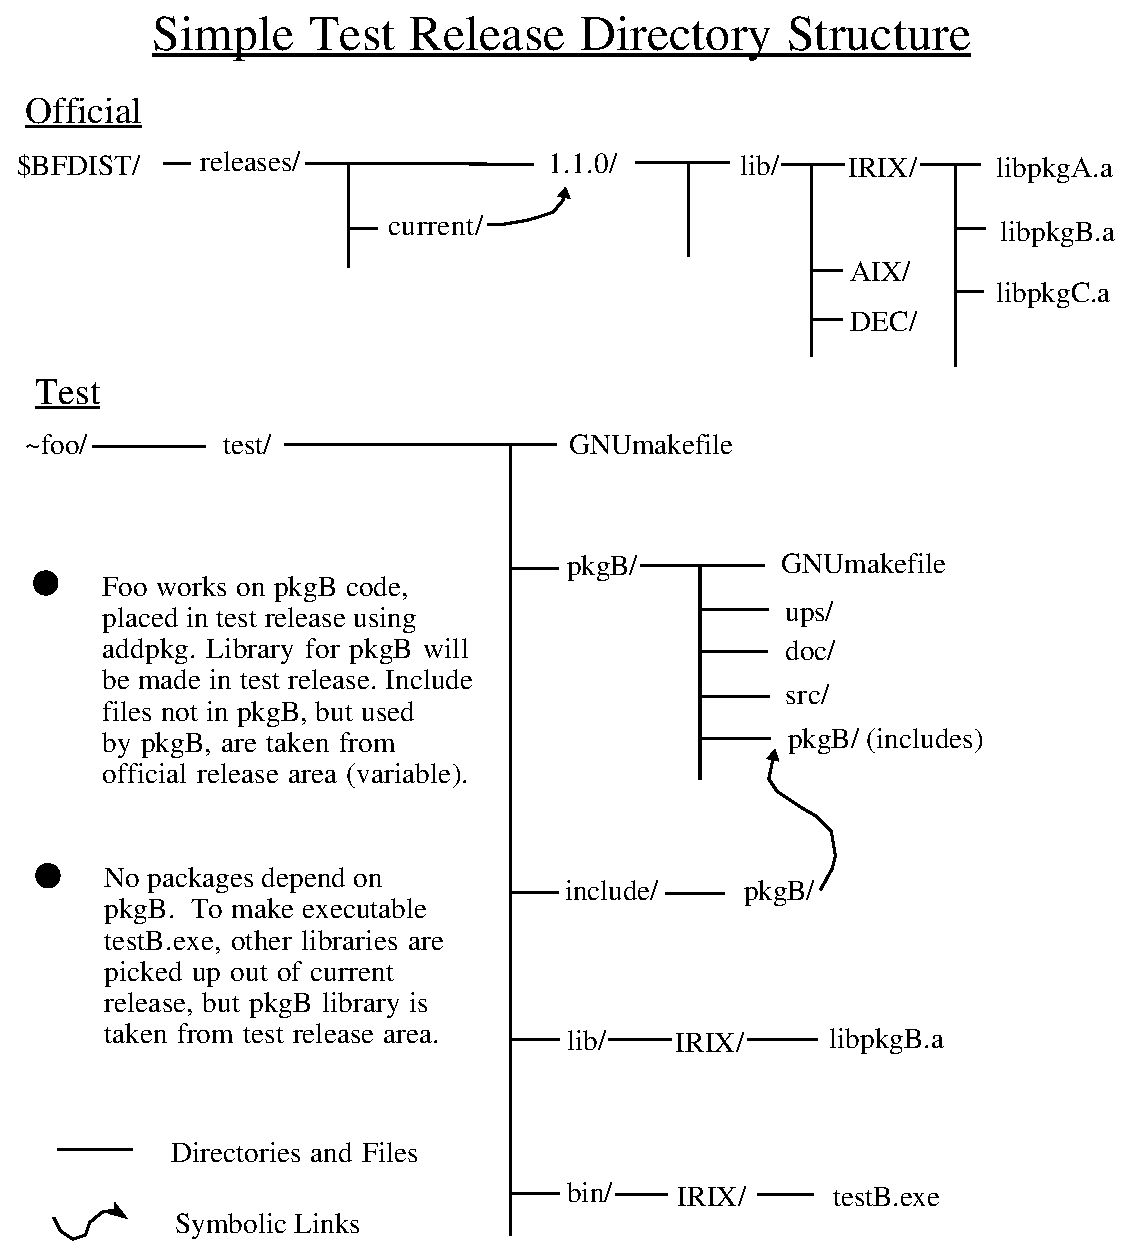
\includegraphics[width=5in]{run_2_dev_simple.eps}}
\caption[Simple Test Release Directory Structure]{ 
Diagram of a simple test release directory structure, and how it relates to the
official release directory structure.  Here the package ``pkgB'' is being
developed\index{packages!development of}, but since nothing else depends on pkgB, all other include files
\index{dependencies!simple test release} 
and libraries are taken from the current official release.}
\label{fig_dev_simple}
\end{figure}
\clearpage 

\vspace*{1.0in}
\begin{figure}[bht!]
%\epsfysize=8in
%\epsffile[36 54 581 756]{run_2_development.ps}
%\centerline{\epsfig{figure=run_2_development.eps,width=5in}}
\centerline{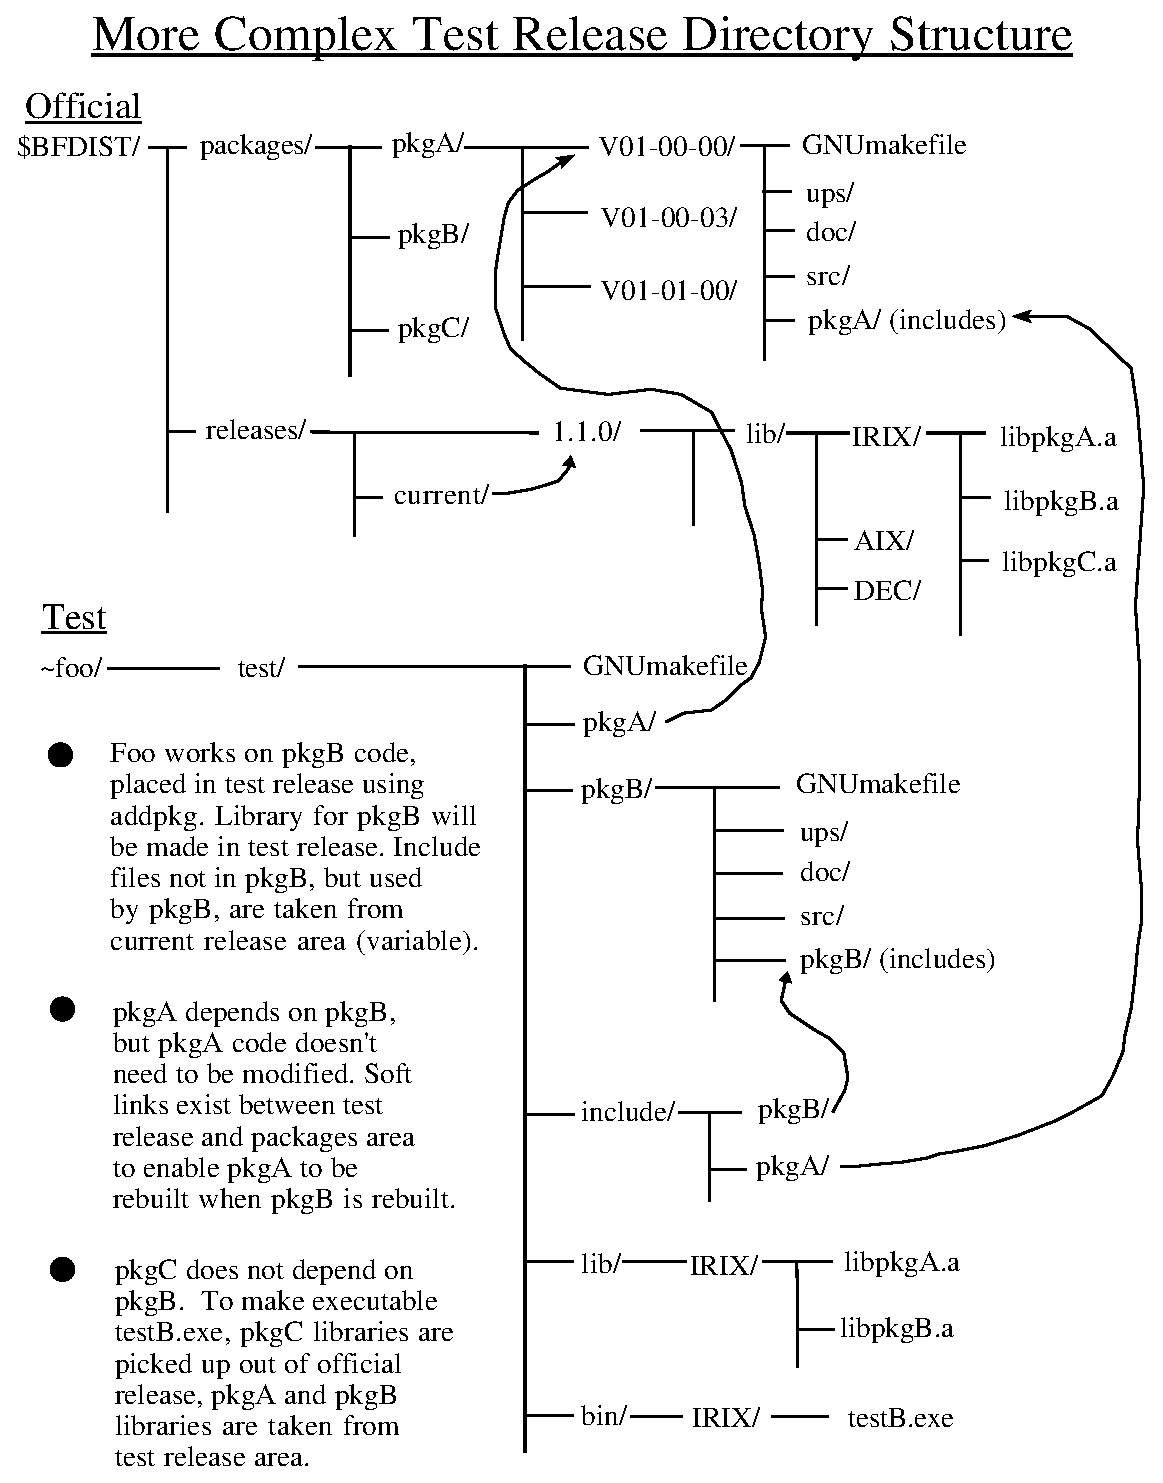
\includegraphics[width=5in]{run_2_development.eps}}
\caption[Complex Test Release Directory Structure]{ 
Diagram of a complex test release directory structure, and how it relates to the
official release directory structure.  Here the package ``pkgB'' is being
developed\index{packages!development of} , and ``pkgA'' depends on the contents of ```pkgB''. The curved lines 
\index{dependencies!complex test release} 
correspond to soft links.}
\index{soft links}
\label{fig_testrel}
\end{figure}
\clearpage 

\subsection{Distribution}
Initial distribution of the offical release structure to a remote machine will 
eventually be done via UPD once we have fully integrated it into our system.
In the meantime, we have developed simple scripts to 
initially distribute the release structure to a remote machine, 
discussed in Appendix~\ref{app_dist}.  
The release structure, those directories and soft links underneath
\index{soft links}
\$SRT\_DIST/releases in Fig.~\ref{fig_directory}, are saved in a tar file on the
server\index{client-server} machine.  
In addition, each package\index{packages!tar files}  is saved in it's own tar file. 
The location of the tarfiles on the distribution server\index{client-server} 
machines is given in ???
The
remote manager uses UPD, or currently the shell scripts described in 
Appendix~\ref{app_dist}, to copy these tar files from the distribution machine
to the remote machine and unwind them into the official 
releases\index{releases!area}  and packages\index{packages!area} 
area.  The tar file of the release specifies the flavor of the operating system and 
the version of the release. The user sets up the release using UPS as 
\index{UPS}
described in Section~\ref{sec_setup}.  The philososphy of using UPS with the
system is discussed in Appendix~\ref{app_ups}.

Once the remote machine has received an initial distribute of an official 
release, linking and development can take place. 
Distribution of the source code to a remote machine for user development is
accomplshed via SoftRelTools.  As described in section~\ref{sec_debug}, 
addpkg\index{addpkg} 
is used to checkout a complete package from CVS\index{CVS} for user development 
of that package\index{packages}. Within a test release, developers can
build and link code with their changes.  Libraries and include files from
other packages are taken from the official release. A development
release, described in section~\ref{sec_development}, can be constructed on 
any node and the code can be updated daily via CVS and rebuilt.  This is a
simple way of distributing the code to remote institutions on a daily basis,
and insuring that it works there just as well as on a central system. For
instructions on distribution of the development release at CDF, please see
section~\ref{sec_distribution_development}.

In summary, distribution of binaries and code of official 
releases\index{releases} takes place 
with UPD, after which users can link, and developers can work 
\index{linking!and distribution}
on packages  distributed to their test release by SoftRelTools.

%================================================================================
% All the appendices
%================================================================================

\clearpage
{\Huge \flushleft Appendix}
\appendix

%%%%%%%%%%%%%%%%%%%%%%%%%%%%%%%%%%%%%%%%%%%%%%%%%%%%%%%%%%%%%%%%%%%%%%%%%%%
% CVS
%%%%%%%%%%%%%%%%%%%%%%%%%%%%%%%%%%%%%%%%%%%%%%%%%%%%%%%%%%%%%%%%%%%%%%%%%%%
\section{Appendix on Version Control with CVS}
\label{app_cvs}

Concurrent Versions System (CVS)\index{CVS!introduction} is a 
freeware version control system that is widely
used by freeware developers including those in high energy physics. 
It is used by the CERN and Fermilab computing
divisions and by the following physics collaborations: ATLAS, CMS, SDSS, NuTeV,
CLEO, and BaBar.  Now it is also being used by CDF, D0 and BTeV. 
\index{BaBar}
\index{CDF}
\index{D0}
\index{BTeV}

Additional information can be found at:

\begin{itemize}
\item CVS Documentation <http://www.fnal.gov/docs/products/cvs>
\item CVSH <http://www.fnal.gov/cd/FUE/cvsh/>      
\end{itemize}

\subsection{ The CVS Repository and Basic Concepts}
\index{CVS!introduction|(}

CVS\index{CVS!repository} extends the notion of revision control from
a collection of files in a single directory, as in CMS, to a hierarchical
collection of directories each containing revision controlled files.
For example, two CVS\index{CVS!repository} repositories designed to contain the CDF offline software
\index{CDF}
\index{CDF!repositories}
are shown in Fig.~\ref{fig_repository}.      


\begin{figure}[tbh]
\begin{center}
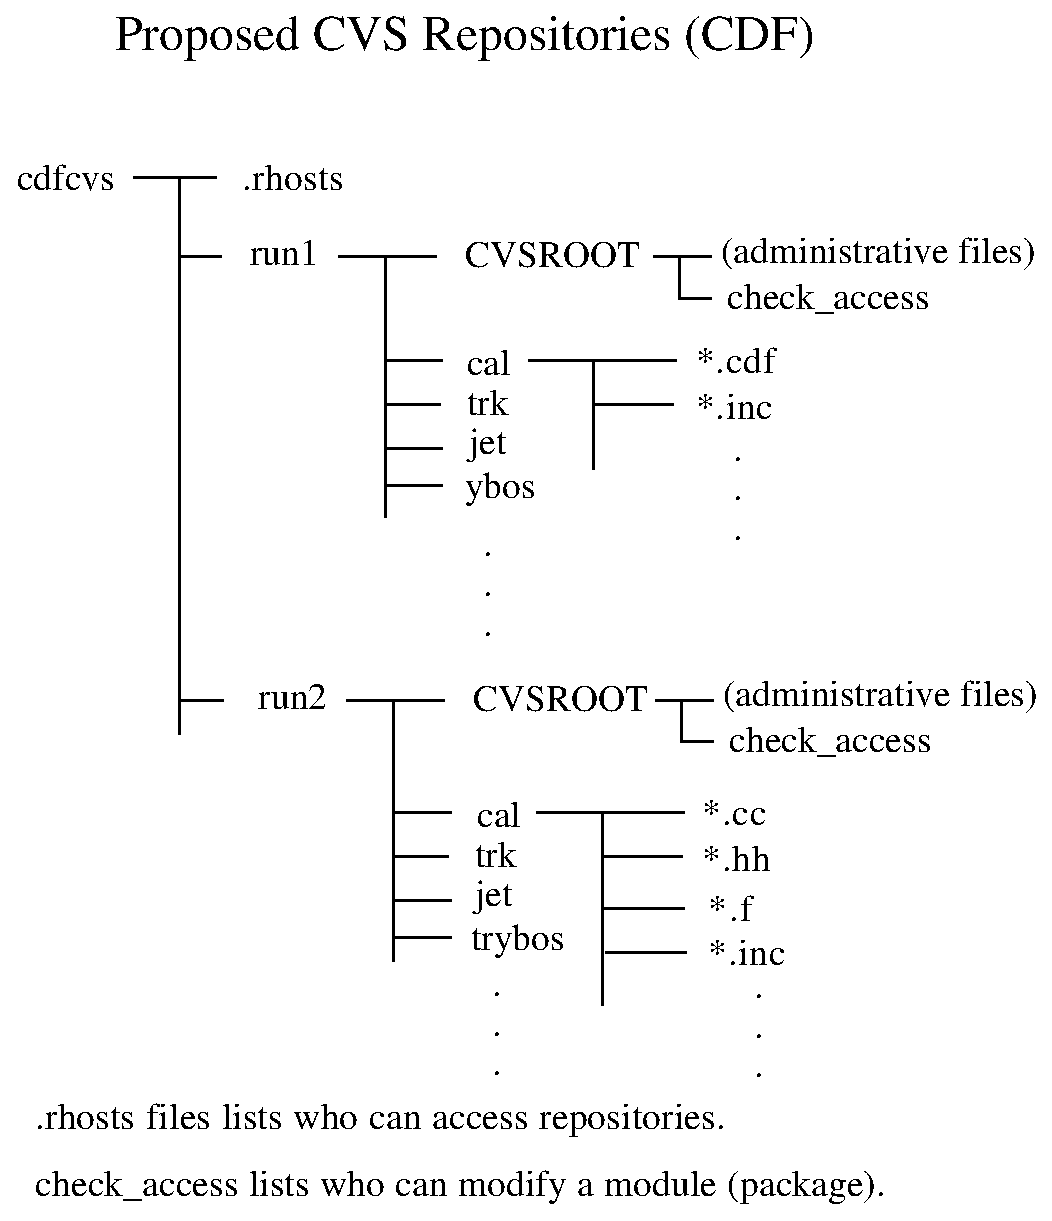
\includegraphics[width=4.0in]{two_repositories.eps}
\end{center}   

%\vspace*{-0.5in}
\caption[CVS Repositories]{
The structure of two CVS\index{CVS!repository} repositories, one for run 1 and one
for run 2.}
\label{fig_repository}
\end{figure}

Like CMS groups, CVS\index{CVS!module} collects files together into {\em modules}, and allows
operations on entire modules.  For example, the jet library would be a
module. Like a CMS class, CVS\index{CVS}
allows a collection of specific file versions to have a name, called a
{\em tag}.  CVS\index{CVS!file versions} labels each file with version
numbers, and allows branches and merging as depicted in Fig.~\ref{fig_branch}.
\begin{figure}[tbh]
\begin{center}
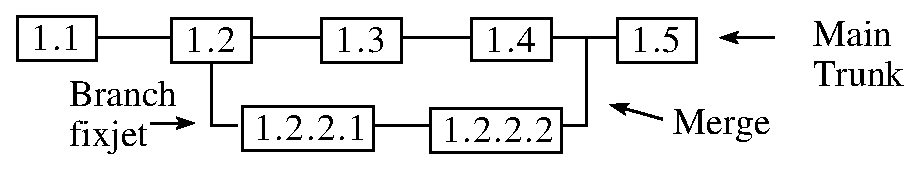
\includegraphics[width=6in]{cvs_revisions.eps}
\end{center}
\caption[Revisions, Branching and Merging]{
The versions of a particular file along the main trunk of the revision,
1.1, 1.2, 1.3, 1.4 and 1.5 are shown, along with a branch called {\ttfamily
fixjet},
that consists of modifying revision 1.2 into 1.2.2.1 and 1.2.2.2.  The
branch was merged back into the main trunk after revision 1.4 was complete,
giving revision 1.5.}
\label{fig_branch}
\end{figure}
As its name indicates, CVS\index{CVS!concurrent development} encourages concurrent revision by multiple
developers in parallel, unlike CMS which is designed for linear revision of
reserved files.  A script has been written to allow the command {\ttfamily
reserve} in CVS\index{CVS!reserve script} if desired.

\subsection{ Basic CVS Commands: A Single Revision Cycle}

As an example for the CVS\index{CVS!revision cycle} novice, the following commands perform a single
software revision cycle:
\begin{quote}
\ttfamily
cvs checkout jet/jtc90s.F\index{CVS!commands!checkout} \\
cd jet \\
cvs log jtc90s.F\index{CVS!commands!log} \\
emacs jtc90s.F \\
cvs commit -m "Changed jet energy scale!" jtc90s.F\index{CVS!commands!commit} \\
cd .. \\
cvs release -d jet \index{CVS!commands!release}\\
\end{quote}
The {\ttfamily cvs checkout}\index{CVS!commands!checkout} command creates in the users working directory a
subdirectory \texttt{jet/}, and places in \texttt{jet/} the file
\texttt{jtc90s.F}. This is like {\ttfamily CMS fetch} with an additional directory structure
created. The user goes to the \texttt{jet/} subdirectory and issues the
{\ttfamily cvs log} command\index{CVS!commands!log}, which presents her with the history of the file
\texttt{jtc90s.F}, like {\ttfamily CMS history}. The user then edits the file
(in this case using \texttt{emacs}) and places the file
back in CVS using {\ttfamily cvs commit}\index{CVS!commands!commit} and including comments, like
{\ttfamily CMS replace/keep}.  Finally the user passes back up to the working
directory and removes the entire jet/ directory tree with the command
{\ttfamily cvs release -d}\index{CVS!commands!release}, which checks to make sure there aren't any changes  
left to incorporate before deleting the files.
\index{CVS}
\index{CVS!introduction|)}

%%%%%%%%%%%%%%%%%%%%%%%%%%%%%%%%%%%%%%%%%%%%%%%%%%%%%%%%%%%%%%%%%%%%%%%%%%%
% Structure
%%%%%%%%%%%%%%%%%%%%%%%%%%%%%%%%%%%%%%%%%%%%%%%%%%%%%%%%%%%%%%%%%%%%%%%%%%%
\clearpage
\section{Appendix on the SRT Software Release Directory Structure}
\label{app_structure}

    To accommodate the storage of the various components of such a release, 
a consistent tree-structured hierarchy of directories is established. 
For expository purposes, we identify each directory with its depth (distance 
from the base) in the hierarchy. All quoted file names correspond to the 
labels in Figure~\ref{fig_directory}.

\subsection{The root directory (depth 0)}

    At the base (root) of this hierarchy is a single directory. Labelled 
``\$SRT\_DIST/'', this directory's sole purpose is to provide a starting point for 
the structure. In this root directory are entries for (the directories at the 
roots of) the two major subtrees of the structure, ``packages/''
\index{packages!area} 
 and ``releases/"\index{releases!area}. 

\subsection{The ``packages/'' directory (depth 1)}

    This directory serves as a root for the source code, documentation, 
makefiles, etc., for all versions of all packages in the product. Thus, each 
entry in ``packages/''\index{packages!area} is the starting point for a particular package. Note 
carefully that only items from the CVS\index{CVS!repository} repository are found. 

\subsubsection{Package directories ``pkgA/'', ``pkgB/'', ... (depth 2)}

    Each of these directories, direct descendents of ``packages/''
\index{packages!area} , serves as the
root of all the code, etc., associated with all versions of a single package. 
These directory names typically match the corresponding CVS\index{CVS!module} module name. Each 
such directory will have as many entries as the package has versions. 

\subsubsection{Individual version directories ``V01-00-00/", ... (depth 3)}
\label{sec_version}

    Each distinct version of a given package has its own root directory, a 
direct descendent of the package's root at depth 2 described above. The name 
of a version directory typically matches the release tag associated with the 
corresponding versions of the files in the CVS\index{CVS!tag or version} repository. 

\subsubsection{Depth 4 and beyond}
\label{sec_depth4}

    At this level, we find the source structure corresponding to (directly 
descended from the version root of) a particular version of a particular 
package. Among these entries, we might typically find: 
\begin{enumerate}
\item ``GNUmakefile'' (for the complete package)\index{packages!GNUmakefile} , 
\item  ``ups/'' (directory holding setup and unsetup files).
\index{UPS!subdirectory}
\item ``doc/'' (directory for tutorial and other documentary files), 
\item ``man/'' (directory to contain Unix-style man pages), 
\item ``src/'' (directory containing .cc and .f files), 
\item ``include/'' (directory holding .h and .inc files), 
\end{enumerate}

    Note: Figure~\ref{fig_directory} does not show all these directories, but 
they are clearly implied by the accompanying narrative. Also, 
Figure~\ref{fig_directory} labels the ``include/'' directory with the 
package name; however, this name is not a requirement of the structure but one which we 
recommend. This is because it reflects the including convention adopted in
the code: \#include pkgname/incname (see section~\ref{sec_include}).  

Recall that binary files are not intended to be located here.
However, one could conceive of additional directories here, such as ``test/'' or 
``examples/'' or ``tools/'', not necessarily part of all packages.

    The guiding principle is that, at this level, the logical structure of a 
package ought to dictate the directory structure. For reasons to become clear 
shortly, the ``include/'' directory is required, and must contain all those 
files that are visible to, and hence may be included by, any other packages or 
user software. 

The Unix-style man pages are put in the ``man/'' area of the directory 
structure. The UPS project setup file modifies the users MANPATH to include 
\index{UPS!MANPATH}
this area.

\subsection{The ``releases/'' directory (depth 1)}

    This direct descendent of the product root directory serves as a base for 
all vetted releases of the product. Each entry in this directory is the 
starting point for one such release. 

\subsubsection{Individual release directories ``1.0.0/", ... (depth 2)}

    Each of these directories, direct descendents of ``releases/", serves as the
root of all the information needed to make use of a release of the entire 
product. The name of a release directory typically matches the identification 
of a release in terms of the collection of all sources. 

    In addition, there are two standard directory names found at this level: 
``production/'' and ``current/''. These are only links to other release 
\index{soft links}
directories. They serve, however, as convenient and standardized labels so 
that users need not necessarily be cognizant of new releases: as each new 
release is installed, these directory links are intended to be broken and 
re-created as appropriate.\index{releases!soft links}

    At this level a general makefile can be created automatically to build the 
entire release tree. The makefile will simply: 
\begin{itemize}
\item invoke each of the package-specific makefiles\index{packages!GNUmakefile}  
(previously described) in turn, and 

\item install the resulting libraries and binaries into the respective 
``lib/'' and ``bin/'' flavor-specific subdirectories. 
\end{itemize}
\paragraph{\underline{Release component package directories ``pkgA/", ... (depth 3)}}

    Each of these directories corresponds to one of the 
packages\index{packages}  that make up 
the release, reflected by their parent directory, of the product. These 
directories are named for their corresponding packages. 

    However, in order to reduce unnecessary duplication of information already 
present within the ``packages/'' substructure, each of these directories is 
simply a link to the directory (at depth 3, described in 
\index{packages!soft links} 
\index{soft links}
section~\ref{sec_version} above) corresponding to the appropriate version of 
the package used to construct this release. 

\subsubsection{The ``include/'' directory (depth 3) and its descendents}
\label{sec_include}

    The intent of this directory, also a direct descendent of an individual 
release directory, is to serve as the indirect base for all .h files that 
are intended to be visible to any user of the software product. 

    This ``include/'' directory contains links, named for the individual 
\index{soft links}
\index{packages!soft links} 
packages, to the various depth 4 ``include/'' directories found under the 
``packages/'' structure (described among section~\ref{sec_depth4} above). In 
this way, code duplication is avoided, yet all include files are accessible to 
the user from one convenient source. 

The convention for including files in the source code is
 \#include pkgname/incname.
Here an 
include file, incname, is associated with a unique package, pkgname, necessary 
if two packages\index{packages!include files} have different include files with the same name.      

\subsubsection{The ``lib/'' and ``bin/'' directories (depth 3)}

    Via these directories, the remaining direct descendents of an individual 
release directory, we find a path to the software product's binaries. As is 
traditional, executables are found under ``bin/", while user-linkable libraries 
\index{linking!library locations}
are found under ``lib/". 

\subsubsection{Flavors directories ``IRIX/", ``AIX/'', ... (depth 4)}
\label{app_flavors}

\begin{sloppypar}
    These directories come into play when the software product is supported on
multiple platforms. When such is the case, ``bin/flavor/'' would serve to 
consolidate all executables for a given platform, while ``lib/flavor/'' would 
play a similar role for user-visible libraries. 
The directory is actually given a name that is a concatenation of the flavor
and version of the operating system, for example IRIX5 instead of IRIX.
This name (e.g. IRIX5) is stored in the environmental variable \$SRT\_ARCH.
\end{sloppypar}

\subsection{Usage of the directories}

    In the following sections we explain how the SRT directory structure and 
its Software Release Tools are envisioned to relate to the various client 
communities that deal with them. 

\subsubsection{A user's viewpoint}

    The UPS setup of a particular release sets the user's path, manpath, etc., 
\index{UPS!MANPATH}
\index{UPS!PATH}
in such a way that binaries are directly accessible, include files can be 
available through an environment variable pointing to the release ``include/'' 
tree, and the libraries can be used by a reference to the library tree 
environment variable via the ``-L'' compiler option. 
\index{compiler!options}

    The directory structure assumes that most users will make use of a complete
release, rather than mixing-and-matching packages across releases. If, however, 
a user would like to work with release ``A'' of a product but use version ``B'' of 
a package ``pkgC'', s/he should use the SRT ``newrel'' command to recreate the 
\index{newrel!users viewpoint}
release structure in his/her own working directory. To this command the user 
has to specify version ``B'' of package ``pkgC''. Version ``B'' of pkgC needs to 
be built in this new test release context. The user can then link his/her own 
\index{linking}
executable against this new test release. 

\begin{sloppypar}
Those users who want to write their own scripts and makefiles just need to 
know a few things. As discussed in section~\ref{sec_setup}, the UPS setup 
\index{UPS!SRT\_DIST and SRT\_CURRENT}
\index{UPS!environment}
defines the environmental variables \texttt{SRT\_DIST} and \texttt{SRT\_CURRENT}.  
The environmental variable \texttt{SRT\_ARCH} is also defined to indicate the flavor 
of operating system, as discussed in appendix~\ref{app_flavors}. In principal,
these are the only environment variables you need to use the software release 
structure. Although we strongly recommend the use of our setups and makefiles, 
the user is free to suitably define these variables to point at the right areas,
and then write their own scripts and makefiles.  The user needs to know 
that compilation with package include files\index{packages!include files}  is 
accomplished using the compilation option 
\texttt{-I\$SRT\_DIST/releases/\$SRT\_CURRENT/include}, and linking with package
\index{linking!-L option}
libraries is accomplished using the link option 
\texttt{-L\$SRT\_DIST/releases/\$SRT\_CURRENT/lib/\$SRT\_ARCH}. Users who 
prefer to do it themselves should be able to use this information to write 
their own sripts and makefiles.  However, we recommend that the provided
scripts and makefiles be used.
\end{sloppypar}

\subsubsection{A developer/contributor's viewpoint}

    In a private ``workdir'' directory, using the command ``newrel'' the developer 
\index{newrel!from developers viewpoint}
can recreate the release structure starting from a reference release. 
To modify an existing package,  the contributor can use the ``addpkg''
\index{addpkg!from developers viewpoint} command 
that checks out the module from the CVS\index{CVS!repository} repository. 
The checkout command creates the main directory structure for the package 
reflecting the module organization in CVS. Extra directories need to be 
created by the package-specific make file. The developer then 
communicates changes to the librarian, who commits them to CVS\index{CVS}.

\subsubsection{A librarian/package manager's viewpoint}

\begin{sloppypar}
    A librarian has to go through the same steps a developer goes through, but 
he has write access to the CVS\index{CVS} repository for his own 
package\index{packages!librarian}. The librarian has access to the package-specific directory in the 
\$SRT\_DIST/packages tree. This can be accomplished via a group uid, and 
trusted developers can be added or removed from this uid using the systools
commands \texttt{cmd addmember} and \texttt{cmd delmember}.
\end{sloppypar}

\subsubsection{A product/configuration manager's viewpoint}

    The product manager has write access to the entire \$SRT\_DIST tree. He can 
operate directly in the \$SRT\_DIST directories and use the ``-p'' (production) 
option of the ``newrel'' command. 
\index{newrel!managers viewpoint}

%==========================
% UPS and SRT
%==========================
\section{Appendix Using UPS with SRT}
\index{UPS}
\label{app_ups}
 
First some general comments. It is important to note that much of the 
information about which package\index{packages} 
    version works with what other package version, is contained in the release 
directory structure itself. This
    removes the requirement that this information be stored in the UPS database
\index{UPS!databases}
as dependencies. This is
\index{dependencies!UPS}
    desirable for a number of reasons. Maintaining and distributing this 
information in the form of the UPS 
    database has through the years proven to be difficult. Various recent 
additions to UPS help - cups is an
\index{UPS}
    example - but it is still true that you must be a UPS expert in order to 
\index{UPS}
effectively maintain this information. In
    a period of stable code distributions this is not a disaster; however, in a 
heavy development period it may
    become one. The other reason for minimizing UPS's knowledge of package 
\index{packages!UPS}\index{UPS}
dependencies is that it will
\index{dependencies!UPS}
    speed up and simplify the process of setting up a set of packages.
\index{packages!setup}  There 
will be fewer ambiguities about
    which versions of packages actually get setup. 

    However the concept of UPS product dependencies is still needed. There are 
\index{dependencies!UPS}
many products that we use, over
    which we have little or no control. In fact any 
package for which we do not keep
    our own CVS\index{CVS!external packages} library, would be classified in this category. Let's call 
them external packages\index{packages!external}. Examples
    would be products like cernlib or tcl/TK. These packages do not live in the 
directory structure,
    and therefore the older mechanisms for handling dependencies are still required. 
\index{UPS}
\index{dependencies!UPS}
Hopefully the coupling between
    this class of packages\index{packages!inderdependencies}  is not strong. For instance, no one would be happy if
you could only use version A of
    tcl/Tk with version B of cernlib. Also, note that references to libraries and 
binaries from this class of package are still referred to through environmental 
variables or path setting. They are not copied to the
 \verb|$SRT\_DIST/release/<version>/lib| or \verb|$SRT\_ROOT/release/<version>/bin| areas. 

\subsection{Using UPS for packages}
\index{packages!UPS} 
\index{packages!setup} 
\index{UPS!package setup}
\index{UPS}

    Packages inside the directory structure still need to be able to 
specify how environment variables,
    needed for the running of their package, must be set. For example, in the 
news product, NNTPSERVER
    must be set to the site news server machine; for tex, TEXINPUTS defines the
search list of directories to
    look for tex files. Many of the other uses of ups/setup.* files, like path 
\index{UPS}
modifying, are not needed by this type
    of package because all of the binaries live in the release structure. 
Therefore, for each
    package in the package tree, at the same level as doc, src, include and 
GNUmakefile, there is a UPS 
\index{UPS!subdirectory}
    subdirectory, which contains setup and unsetup files that are 
fragments of the
full project setup. These fragments are concatenated into the full setup 
and unsetup files in the release tree during the release build. 
Each of the fragments is a fast
equivalent of \texttt{setup <pkg>} with the appropriate version number.

\subsection{Using UPS with releases}
\index{UPS!release setup}

    In the release tree there is a UPS subdirectory at the same level as 
\index{UPS!subdirectory}
bin, lib, and include. It 
    contains a setup file that sets the path to contain the bin area of the
release and define anything else
    needed for the global release. 
From now on we refer to a global release
as a project. Thus a project is a set of experiment written products that 
get linked together into executables, and hence would form a release.  For
example online and offline could be separate projects.

The setup and unsetup file also have copied into them the 
fragments from all of the packages\index{packages!setup fragments} 
    contained in the release. These files could be built by the script that 
makes new releases\index{releases} (newrel), but currently they are build by the release 
manager by declaring the release of the project to UPS.  Marc Mengel has 
\index{UPS}
developed a utility called
\index{newrel!ups}
UPS\_COMPILE which we use to collect the fragments together into a 
\index{packages!UPS compile} 
\index{UPS!compile}
single script. The setup file
    also declares this release to the experiment UPS database so that users of 
\index{UPS!databases}
the release could say, for example, ``setup $<$project$>$ 
[$<$project-version$>$]'', as is done in section~\ref{sec_setup}.
At this time any external package dependencies could be
\index{dependencies!UPS}
defined in the UPS database.

\subsection{External Packages and UPS}
\index{packages!external} 
Not all packages used by the experiment will be included in the release 
structure. External packages, such as CERNLIB or tcl/TK or gcc, for which we 
do not usually rebuild the code, are not located in the release structure.  
They are located somewhere else which is pointed to by the normal UPS 
\index{UPS!external packages}
environmental variable.  We do not use CVS\index{CVS!external packages} to track the source code of external 
packages. There is no restriction on where the environmental variable 
\texttt{<product>\_DIR} points. If we need to rebuild external packages, we
use their own makefiles, not the SoftRelTools makefiles.

In the SoftRelTools makefiles we use the UPS \texttt{<product>\_DIR} 
\index{UPS!product variable}
environmental variables
\index{packages!external!environmental variables} 
to pickup external package libraries and include areas necessary for building.
These environmental variables may be defined through UPD dependencies, whereby
\index{dependencies!UPS}
we have declared the project to depend on a given version of an external 
package. The intent is that \texttt{<product>\_DIR} is set when we setup the
project, not via a separate ``setup $<$product$>$'' statement which might 
pickup the wrong version of the external product for the project.

%%%%%%%%%%%%%%%%%%%%%%%%%%%%%%%%%%%%%%%%%%%%%%%%%%%%%%%%%%%%%%%%%%%%%%%%%%%
% Makefiles
%%%%%%%%%%%%%%%%%%%%%%%%%%%%%%%%%%%%%%%%%%%%%%%%%%%%%%%%%%%%%%%%%%%%%%%%%%%
\section{Appendix on Makefiles in Software Release Tools}
\label{app_make}

SoftRelTools use GNU Make for building libraries and executables.
\index{gmake}
\index{gmake!GNUmakefile!user run2}
The file GNUmakefile, in the area where the gmake command
is given, tells GNU Make what to build.
%The user only needs to use
%the makefile in section~\ref{app_user_make} to link a job, and shouldn't need
%to modify it.
\index{linking}
The developer introducing a new package, or the user trying to link an
executable, needs to modify simple
makefiles described in section~\ref{app_package_make}.  Developers, code
librarians, and code managers will want to be aware of the
makefiles discussed in section~\ref{app_release_make}, but should
not need to modify them.   

\subsection{Package Makefiles}
\label{app_package_make}
\index{packages!GNUmakefile}
The following example of package makefiles, \\
\$SRT\_DIST/releases/\$SRT\_CURRENT/Framework/GNUmakefile 
and \\ \$SRT\_DIST/releases/\$SRT\_CURRENT/Framework/src/GNUmakefile, 
are used for building the libraries and executables of the Framework package.
\index{gmake}
\index{gmake!GNUmakefile!package level}
They are examples of typical package makefiles used by gmake in the examples of 
section ~\ref{sec_debug} and ~\ref{sec_newrel}. 
The first makefile only points gmake at the subdirectory src in which the
\index{gmake}
second makefile resides. The second makefile specifies the library target 
libapp.a, and includes the architecture specific makefile for the tcl package, 
on which the framework package depends.  Both makefiles include standard.mk 
which defines the compilation and dependency generation in detail.
\index{BaBar}
\begin{footnotesize}
\begin{verbatim}
$SRT\_DIST/releases/$SRT\SRT\__CURRENT/Framework/GNUmakefile 
# GNUmakefile for the BaBar Framework package
#
# uses SoftRelTools/standard.mk
#
#    Bob Jacobsen, Jan 96
#
#############################################################
# file lists (standard names, local contents)

# include file products
INC =

# library product
LIB =

#library contents
LIBFFILES  =
LIBCFILES  =
LIBCCFILES =

# subdirectories
SUBDIRS = src

# binary products
BINS =

############################################################
include SoftRelTools/standard.mk
\end{verbatim}
\end{footnotesize}
\vspace*{1in}
\begin{footnotesize}
\begin{verbatim}
$SRT_DIST/releases/current/Framework/src/GNUmakefile 
# new Makefile for Framework - the old one is unchanged.
#
# uses SoftRelTools/standard.mk
#
#############################################################
# file lists (standard names, local contents)

# include file products
INC =

# library product
LIB = libapp.a

#library contents
LIBCFILES  =
LIBCCFILES := $(shell ls *.cc)


# binary products
BINS =

# APPMain.o is required for Solaris link
all:
lib: $(libdir)/APPMain.o
$(libdir)/APPMain.o: $(libdir)/$(LIB)
        cd $(libdir); ar x $(LIB) APPMain.o
include SoftRelTools/arch_spec_Tcl.mk

############################################################
include SoftRelTools/standard.mk
\end{verbatim}
\end{footnotesize}


\subsection{Release, Standard, and Architecture Specific Makefiles}
\label{app_release_make}
At the top of every release is a GNUmakefile as shown in 
Fig.~\ref{fig_directory},~\ref{fig_dev_simple}, and ~\ref{fig_testrel}. The 
release makefile recognizes the experiment by 
means of the .experiment file, which contains names like CDF or D0. The release
\index{CDF}
\index{CDF!.experiment file}
\index{D0}
\index{D0!.experiment file}
\index{.experiment file}
makefile specifies what areas will be searched for include files when
compiling, and what areas will be searched for libraries when linking.
\index{linking}
Most important, for the library and executable targets, this file effectively 
loops over the individual package makefiles and runs make for them.
The release makefile is the heart of the building system.

The user makefiles and package makefiles described in the last section
includes the makefile standard.mk.  This makefile contains standard target 
definitions and rules for compilation and linking.  Similarly, standard.mk
\index{linking}
includes the file arch\_spec.mk, which contains the architecture specific
rules for each machine and operating system.
\clearpage



\clearpage
\addcontentsline{toc}{section}{References}
\begin{thebibliography}{99}

\bibitem{ref_sdss} CVS at SDSS is described on the Code Management WWW pages
at http://www-cdf.fnal.gov/offline/code\_management/sdss.html.
\index{CVS!SDSS-CVS}

\bibitem{ref_babar1} Bob Jacobsen, ``The BaBar Software Release Structure'',
\index{BaBar}
March 5, 1995, on the WWW at
http://www.slac.stanford.edu/BFROOT/dist/releases/current/SoftRelTools/ 
SoftRelToolIntro.ps.

\bibitem{ref_babar2} Bob Jacobsen, ``Using the BaBar Software Release 
Structure'', October 28, 1995, 
http://www.slac.stanford.edu/BFROOT/doc/Computing/Reconstruction/Notes/
SoftRelToolUser.ps.

\bibitem{ref_tuura} Lassi A. Tuura, ``Helper programs for Moose Directory
Structure'', http://wwwcn1.cern.ch/l/lat/www/notes/soft/dist/scripts.html.

\bibitem{ref_commentary} Walter Brown, Flavia Donno-Raffaelli and Elizabeth
Sexton-Kennedy, ``On the Software Release Directory Structure'' on the Code
Management WWW pages at 
at http://www-cdf.fnal.gov/offline/code\_management/srt.html.

\bibitem{ref_REBUILD} Flavia Donno-Raffaelli, ``REBUILD Users Guide and
Reference Manual'', CDF Note 1611, August 15, 1994.  Available on the WWW at
http://www-cdf.fnal.gov/offline/code\_management/rebuild.mem.

\bibitem{ref_cmgt_c++} See discussion of C++ implications on Code Management
\index{C++}
pages on the WWW at 
http://www-cdf.fnal.gov/offline/code\_management/c++.html.

\bibitem{ref_cvs} Basic information on cvs is available from the man pages 
and at http://fnnews.fnal.gov/cd/UNIX/cvs/cvs.html. The complete manual can
be obtained from http://www.loria.fr/$\sim$molli/cgi-bin/wilma.cgi/doc.
\index{CVS!references}.  A hardcopy of this manual is available in the CDF 
trailers office 149-E.

\bibitem{ref_cyclic} Information on Cyclic Software is available at 
http://www.cyclic.com/.

\bibitem{ref_uaf} ``UNIX at Fermilab'', Computing Division Document GU0001, 
available on the WWW at
http://www.fnal.gov/docs/UNIX/unix\_at\_fermilab/welcome.html

\bibitem{ref_alan} Alan Jonckheere, ``Configuration Management: A Turnkey 
System'', on the WWW at 
http://d0www.fnal.gov/\texttt{~}jonckheere/cmgt/turnkey.html

\bibitem{ref_dcd} Mathew Wicks, ``Fermi UNIX Environment DCD Products User
Guide'', DCD0003, DCD User Guide 3.4, January 19, 1993.

\bibitem{ref_cmgt_draft} ``Run 2 Code Management Report'', by Configuration 
Management Working Group on July 12, 1996, available on the WWW at 
http://fnpspa.fnal.gov/Run2/document.html.
\end{thebibliography}

%Index Cross References
\index{dependency files|see {.d files}} 
\index{deleting|see {removing}}
\index{get ! package|see {addpkg}}
\index{get ! test release|see {newrel}}
\index{information!about release|see {statusrel}}
\index{information!about repository|see {lscvs}}
\index{link ! symbolic|see {soft links}}
\index{link ! soft|see {soft links}}
\index{packages!installing production|see {newver}}
\index{packages!removing production|see {rmver}}
\index{packages!creating release|see {newrel}}
\index{packages!interdependencies|see {depend}}
\index{packages!soft links|see {lnkpkg}}
\index{packages!getting|see {addpkg}}
\index{packages!removing release|see {rmrel}}
\index{release!listing contents|see {statusrel}}
\index{release!creating|see {newrel}}
\index{release!removing see {rmrel}}
\index{removing!releases|see {rmrel}}
\index{removing!packages|see {rmver}}
\index{new ! production package|see {newver}}
\index{soft links!creating|see {lnkpkg}}
\index{compile!UPS |see {UPS}}
\index{UPS!dependencies|see {dependencies|UPS}}
\index{server|see {client-server}}
\index{linking!executable filename|see {EXENAME}}
\index{linking!.opt filename|see {OPTFILE}}
\index{make|see {gmake}}
\index{preprocessor|see {CPP}}
\index{version!control|see {CVS}}

\clearpage
\addcontentsline{toc}{section}{Index}
\documentclass[12pt]{article}
\usepackage{graphicx}
\topmargin -1in
\textwidth 6.5in
\textheight 9.5 in
\oddsidemargin 0.0in
\evensidemargin 0.0in
\baselineskip 14pt
\makeindex
\def\see#1#2{{\em see\/} #1}
\begin{document}
\begin{flushright}
\vspace*{0.5in}
CDF Note: CDF/DOC/COMP\_UPG/PUBLIC/3891 \\
\index{CDF}
D0 Note: 3118f \\
\index{D0}
Computing Division Note: GU0013 \\
\end{flushright}
\vspace{0.5in}
\begin{center}
{\LARGE SoftRelTools User's Guide}\\
\vspace{.5in}
{\large Version 2.0}\\
{\large \today }\\
\vspace{.5in}
{\large Last edited by Margaret Votava}\\
{\large \em Fermilab Computing Division}\\
\vspace{.5in}
{\large for:\\
Dave Adams, Jim Amundson, Jim Bellinger, Walter Brown, Glenn Cooper, 
Flavia Donno-Raffaelli, Lynn Garren, 
Herb Greenlee, Robert Harris, Alan Jonckheere, Robert Kennedy, Arthur Kreymer, 
Qizhong Li, Don Petravick, Ruth Pordes, Lars Rasmussen, 
Elizabeth Sexton-Kennedy, Scott Snyder and Gordon Watts.}
\vspace{.5in}
\end{center}
\begin{abstract}
This is the user's guide for the Fermilab version of Software Release Tools, 
a UNIX based software management system for large, collaborative projects
that is used by several experiments at Fermilab.
The system provides software version control with CVS\index{CVS} 
configured in a client-server\index{client-server} mode.
For management and 
building we have adopted the directory structure and SoftRelTools originally 
developed by the BaBar collaboration. 
The system handles the 
version control, management, building, and distribution of code written in 
Fortran, C and C++. A distinguishing feature of the system is its
\index{C++}
ability to allow rapid asynchronous development of 
package versions, 
which can be easily integrated into complete consistent
releases\index{releases} of the entire offline software.  This 
has reduced the time it takes for new and modified code to be made available to 
users. 
\end{abstract}

\clearpage
\tableofcontents
\listoffigures
\listoftables

\clearpage
\section{Introduction}

This document is the User's Guide for SoftRelTools (SRT). It is meant
to give an overview of the SRT environment and commands
from a code developers point
of view. Code librarians should refer to the SRT Reference Guide for
more detailed explanation of the SRT configuration parameters and commands. 

SRT is very flexible in the style in which it allows developers to operate. 
This flexibility presents a difficulty in writing a general purpose "how to"
User's Guide because each librarian has imposed a cycle that is most 
appropriate for that particular release and a naming convention that
best suits the cycle. Users should refer to the specific instructions 
for a given release for the naming conventions and the development cycle. 

Release specific instructions can be found at:
\begin{itemize}
\item CDF Run 2
\item D0 Run 2
\item SDSS
\item ZOOM
\item BTeV http://www-btev.fnal.gov/internal\_documents/code/code\_management.html
\item Minos 
\end{itemize}

\subsection{What is SRT}

SoftRelTools (SRT) is a toolset for managing large software projects, aka releases,
that consists of smaller units, aka packages, that are developed in parallel
by a diverse programming community. It allows individual developers to 
work on their package independently of the ongoing work in other packages,
and to update the whole project when they are satisfied with their 
modifications. In this way, the developer is responsible for the management
of his individual package, while the release librarian is responsible for 
management of the all the packages as a whole.


\subsection{How to use this document}
This document has been written in the style of a book, or pedagogical users
manual, with discussion and illustrations.  People seeking a general 
overview of the system may want to read the normal sections, omitting the 
appendices.  New users or developers who want to do something with the system 
quickly, and don't want to read much, are advised to follow the examples in 
section~\ref{sec_examples} and Appendix~\ref{app_build}. Those seeking a 
reference manual for answering arbitrary questions about the system will find
it quickest to use the index at the back of the document.  

\subsection{Other light reading}

For sleepless nights:
\begin{itemize}
\item SRT Reference Guide
\item CVS User's Guide http://www.fnal.gov/docs/products/cvs/
\item gmake User's Guide http://www.fnal.gov/docs/products/gtools/make.1.html
\item Barbar SRT document
\item CVSH http://www.fnal.gov/cd/FUE/cvsh/ 
\end{itemize}

\section{Software Release Structure}
The software release structure provides a flexible and easy to use
framework for both releasing and developing code.  Code is typically grouped
into {\em packages}\index{packages!definition}; however, it is essential to have a {\em release} of all 
code in 
all packages. The structure must support simultaneously both
releases\index{releases} of stable versions of the 
packages\index{packages}, and asynchronous development of 
the individual packages themselves.  This is in contrast to a structure which
is oriented solely along the lines of a release, where package versions
are only stamped with the release number. The BaBar software release
\index{BaBar}
structure~\cite{ref_babar1,ref_babar2}, which supports both
asynchronous development of packages\index{packages!asynchronous development} 
and grouping packages\index{packages} into 
releases\index{releases!definition},
is shown in Fig.~\ref{fig_directory}. A commentary on this structure with 
a detailed verbal description of Fig.~\ref{fig_directory} is given in 
Appendix~\ref{app_commentary}.

The environmental variable {\ttfamily \$SRT\_DIST} is used as a root to add flexibility.  
Below it are found separate subtrees for packages\index{packages} and releases\index{releases}. 
Within the
package subtree, each package can contain one or more different {\em versions}.
This allows the package librarians to develop packages 
asynchronously\index{packages!asynchronous development},
and assign the package a version number when the package is ready for use
by others.  Within the release subtree, there is a subdirectory for each
existing release.  A release directory consists of soft links to a set of 
\index{soft links}
consistent package versions, plus the libraries and binaries created from
the release for various machine architectures.  Again, the release manager
can use this to create releases\index{releases} as required.  Links within the release
\index{soft links}
directory can be used to provide default names for particular releases, for
example ``current'' for the release recommended for general use at the present
time.

Notice that the soft links between releases\index{releases!soft links} and 
packages\index{packages!soft links} are
\index{soft links}
to the source code only; the libraries and binaries are native to the release.
This is necessary because in C++ a change to a header file used by package A can
\index{C++}
affect the result in package B which uses package A, even if package B does 
not use the part of the header file that is changed or added.  Unlike common
blocks in Fortran, where you can add to the end of a common block which is
used by many packages\index{packages} and you do not need to recompile all the code, in C++
\index{compile}
\index{C++}
if you modify a header file you have to recompile all the code that depends on 
\index{dependencies!and C++} 
that header file. The only way to insure consistent results when
changing a header file is to rebuild both libraries.  

\begin{figure}[tbh]
%\centerline{\epsfig{figure=run_2_directory.eps,width=4.5in}}
\begin{center}
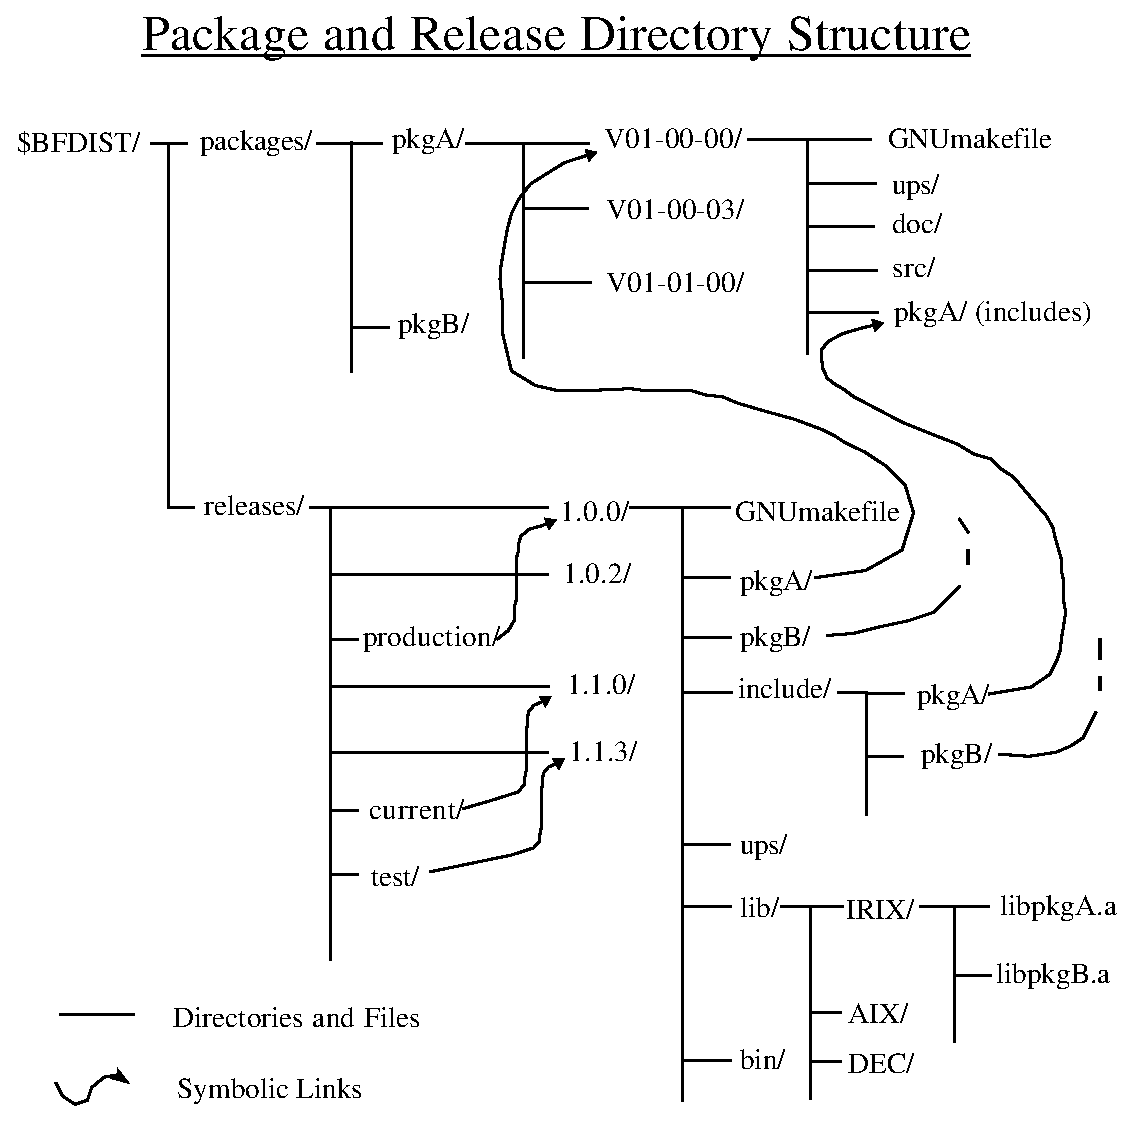
\includegraphics[width=4.5in]{run_2_directory.eps}
\end{center}
\caption[Official Release Directory Structure]{ 
Diagram of the directory structure.  This example includes two
packages: 
``pkgA'' and ``pkgB''\index{packages!definition}\index{packages!figure}. 
The curved lines correspond to soft links\index{soft links} between 
releases\index{releases!definition}\index{releases!figure} and packages.}
\label{fig_directory}
\end{figure}

\subsection{Package and Release Versions and Labels}
\index{version!of package}
\index{version!numbering convention}
The package and release numbering system is designed to allow multiple versions
of packages\index{packages!numbering} and many releases\index{releases!numbering} of code to be available to the collaboration.

The convention for package version numbers is Vxx-yy-zz where
xx is the major version field, yy the minor field, and zz is a bug fix
field incremented for small changes. This version number is also the 
CVS\index{CVS!tag or version} tag of 
that version. The first version is then V00-00-00.
The code manager will install this tag on the initial version of
the code in the repository, and either librarians or the code manager can tag 
subsequent versions using the CVS\index{CVS!commands!rtag} command rtag.

The convention for releases\index{releases!numbering} is x.y.z, where x is the 
major release number\index{releases!major},
y the minor release\index{releases!major}, and z is a bug fix 
number\index{releases!bug-fix}. Thus 1.0.0 would be a major
release that is rigorously tested,  1.1.0 would be a minor release based on 
1.0.0 and would require less testing, and 1.1.3 would be a bug fix or fast 
release based on 1.1.0 and might have almost no testing.  The ``production''
release would generally be a symbolic link to a major release, like 1.0.0.
\index{soft links}
The ``current'' release could be a minor release, like 1.1.0. The ``test'' release 
could be bug fix release, such as 1.1.3.  There could be many major, minor,
and bug fix releases\index{releases!bug-fix}, and only a few of them might have symbolic links pointing
\index{soft links}
to them with names like ``production'', ``current'', ``test'',
``fast-tracking'', etc.
This labelling system allows many different releases, and the level of
validation\index{releases!validation} is apparent from the number.

\subsection{Development Releases}
\label{sec_development}

\index{development} 
In addition to frozen releases with specific versions, SRT structure
also supports a more dynamic development environment. A development release is 
not required, but it is a very useful option for integration, bug detection,
and access to the most recent available code. Most often, 
developers are making changes on different packages in parallel. At
various stages during this development, they will want to share there
work with others. Making a frozen release for each of these stages
would consume a lot of disk space in addition to being a code librarian's
nightmare. 

In Fig.~\ref{fig_development_release} we show the structure of a development
release, which is nearly identical to a frozen release.  The difference is that
the soft links all point to the ``development'' version of the package in the
packages area.  The development version of the package was checked out of
CVS when the package was first added to development, and every day the 
development version is updated via a {\ttfamily cvs update} command. The 
{\ttfamily cvs update} command is a convenient way of distributing 
development, sending only the code that has changed from the repository to the 
development release.  Since we use client-server cvs, all nodes in the system 
are equal, and the process of getting development on a central system is no 
different than the process of getting development anywhere.  Note that no
development actually takes place in the development package area. Developers
are required to develop code in their test releases (see next section) and check
that code back in to the repository, so that the code can propogate to all
development nodes everywhere. 

\begin{figure}[tbh]
%\hspace*{0.1in}
%\epsfysize=6in
%\epsffile[36 100 581 674]{development_release.ps}
%\centerline{\epsfig{figure=development_release.eps,width=4.5in}}
\centerline{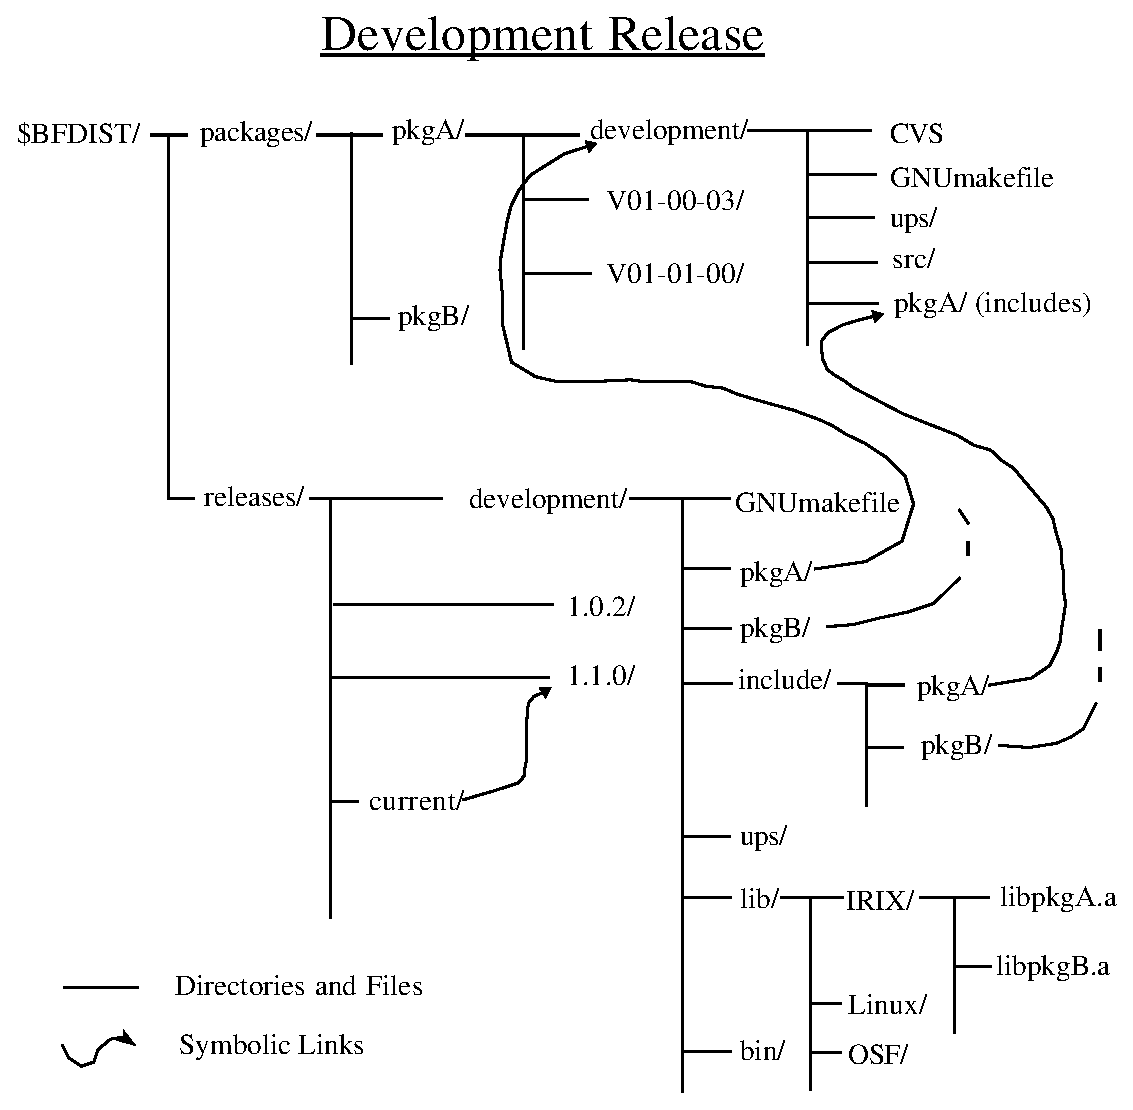
\includegraphics[width=4.5in]{development_release.eps}}
\vspace*{-0.5in}
\caption[Development Release Directory Structure]{ 
Same as Fig.~\ref{fig_directory} except the release called development
contains soft links to the development version of each package, which is 
checked out from CVS and updated from the main repository. There is nothing
hardwired about the tag "development", and each environment may have a 
different term. Please check the specific instructions from your code 
librarian.}
\label{fig_development_release}
\end{figure}

\index{development!update} 
At some interval on each development node 
{\ttfamily cvs update} is done for each package in the release, and 
then the release is rebuilt with the command {\ttfamily gmake}. At
CDF this happens every morning. Developers
can then use the development release to link against.  

A facility exists in 
SoftRelTools to scan the log files that result from the build,
find compilation and linking errors, and send error reports to the designated
developers and package librarians.  
\index{development!error reporting} 
This provides developers with immediate
feedback, and errors are caught and fixed quickly.  
This SoftRelTools error\_reporter facility
also can create error status tables, like the on in Fig.~\ref{fig_status_table}.
Ask your code librarian for links to the location of these log files. 

Although naive users may want to use a frozen release, for stability, 
in a rapidly developing software environment, developers need to use 
the development release to insure that their additions really work with
the most recent software.  

\begin{figure}[tbh]
%\centerline{\epsfig{figure=status_table.eps,width=4.5in}}
\centerline{\includegraphics[width=4.5in]{status_table.eps}}
\vspace*{-4.7in}
\caption[Status Table for Development Release]{ 
Example summary of errors detected during one night's build of the 
Run 2 development 
software at CDF. The lib stage is the compilation stage of the package,and 
the bin stage is the compilation and linking of executables for that package.
A text entry in the table indicates there was an error for the package 
indicated. Here for example there was an error linking an executable in the
TrackingMods package under Linux using the KAI compiler, and no errors 
anywhere else. This summary was generated on Wed Jul 22 08:00:19 1998 by the
error\_reporter facility in SoftRelTools.}
\label{fig_status_table}
\end{figure}

\subsection{Using the Software Release Structure}
\label{sec_examples}

This section will describe the overall procedures needed to develop
in an SRT environment.  In short, a user wants to develop a certain
package. He needs to define a context, or base release, in which this 
package will be compiled and linked. He must define a "test" release
in some working area, then copy the package to be modified
into this working area, and finally set symbolic links for header files
and libraries to the other packages in the base release - see Figure ???. 

The user is afforded many options to globally describe his development 
environment. One of which is a "super" test release. 
Look at figure ???. The default SRT behavior is to define
the path for header files to include both directories in the test 
release as well as the base release. If a user deleted a header file from 
package B in the test release, the make files would still find it in the
base release. This can lead to some confusion. SRT supports the concept
of a "super" test release which will only look for include files in the
test release. It does this by creating a directory called "super" in the
test release and putting links to each pacagke's header files therein. 


The SoftRelTools commands themselves are defined in more
detail in Section ~\ref{sec_commands}. 
Once again, you should
refer to your code librarian's instructions for the naming conventions and
practices unique to your specific configuration. Section~\ref{sec_setup}
describes how to setup SoftRelTools, necessary before any SRT 
commands can be executed.
Section~\ref{sec_debug}                                
describes constructing a test release using {\ttfamily newrel} \index{newrel} 
for development
of a package obtained using {\ttfamily addpkg}.\index{addpkg}  
This is also how a user links a job.
Section~\ref{sec_newver} describes making the new package version official 
using {\ttfamily newver}\index{newver}. Section~\ref{sec_newrel} describes making a new
production release, including the new package version, using {\ttfamily newrel}.

\subsubsection{Setup}
\label{sec_setup}
Because it is flexible and each distribution has opted for different
features, setting up the environment is the most confusing part of using 
SRT. The user needs to work out of a test release. If he doesn't already have
one, he needs to create one with the SRT "newrel" command. This only needs
to be done once, and the user can work from the this area indefinitely. 
Additionally, the user needs to run srt\_setup in each shell that his wishes
to develop in, ie, each time he logs in or creates an xterm. There is a bit
of a chicken and egg problem here in that some srt\_setup switches require that
a test release already have been created (e.g., -A), but you can't create the 
test
release until srt\_setup has been run. The solution is to execute srt\_setup
twice. 

Note that the user can have more than one test release and switch between 
them, but this is not recommended for the novice SRT user. An additional note
is that if you have if you have done an srt\_setup -A and switch test 
releases, you need to run srt\_setup again. 

SRT is very loosely coupled with UPS. It has no requirements on UPS itself,
but is modelled after it. Certain environment variables must be defined, 
e.g., ??? SRT\_DIST in a global file and then srt\_setup run. Code librarians
have wrapped this distribution specific scripts. 
Again, check with your code librarian for your specific instructons. 

For example, below are
the Run 2 setup commands at CDF and D0 (for a more complete list see ???
\index{CDF}
\index{CDF!setup}
\index{D0}
\index{D0!setup}
):
\begin{enumerate}
\item {\ttfamily source /d0library/d0local.login }\\
{\ttfamily setup D0RunII [<base-release>]}\\
\index{D0}
This will setup the D0 Run II software.  
\item {\ttfamily source $\sim$cdfsoft/cdf2.cshrc}\\
{\ttfamily setup cdfsoft2 [<base-release>]}\\
This will setup the CDF Run II software. \\
\end{enumerate}

where the files \texttt{d0local.login} and 
\texttt{cdf2.cshrc} define the UPS databases for D0 and CDF in Run II:
\index{UPS!databases}
\index{CDF}
\index{CDF!UPS databases}
\index{D0}
\index{D0!UPS databases}
the appropriate file can either be sourced 
interactively or in the users \texttt{.login} file.  


How does it know SRT\_DIST???
The setup commands define the  SoftRelTools enviromental variables 
\texttt{SRT\_DIST}, \texttt{SRT\_BASE\_RELEASE}, and \texttt{SRT\_ARCH}. 
\texttt{SRT\_DIST} is the
main directory, \texttt{SRT\_BASE\_RELEASE} is the release 
identifying name
or number in the \texttt{\$SRT\_DIST/releases} directory, and \texttt{SRT\_ARCH} 
specifies the UNIX operating system type and version number.
\texttt{<base-release>} is an optional
argument specifying the release, and if absent will default to the current
release. Note that \texttt{SRT\_BASE\_RELEASE} is not
a pathname.  For example, the \texttt{SRT\_BASE\_RELEASE} release would be found at
\texttt{\$SRT\_DIST/releases/\$SRT\_BASE\_RELEASE}, so \texttt{SRT\_BASE\_RELEASE} could be a name 
like ``current'' or
a number like ``1.0.4''.  In addition, if using in a UPS environment, it 
defines a convenient 
\index{UPS!project variable}
environmental variable (\texttt{<project>\_DIR}, which is 
\texttt{CDFSOFT2\_DIR}, \texttt{D0RUNII\_DIR}, etc.) which 
points at the area \texttt{\$SRT\_DIST/releases/\$SRT\_BASE\_RELEASE}. 
Libraries and include 
files from packages\index{packages} will be taken from the \texttt{<project>\_DIR} area, 
when linking and compiling, unless another area is specified 
by a test release (see section~\ref{sec_debug}). 

\subsubsection{Creating a test release}
\label{sec_testrel}

As previously stated, the user needs to create a working area in which
to make his changes. This is called a test release and is created with
the SRT command newrel.  This command need only be executed once per
test release directory. 

Once the test release is created, the user needs to populate it 
with the particular packages he wishes to modify via the lnkpkg command. 
Let's say that header files in a second package depend on the package the
user wants to modify. The user will want to build the libraries in 
the second package, but not modify the code. He can add the second package
to the test release via the lnkpkg command. 

\begin{itemize}
\item {\ttfamily cd <wherever>}\\
      For example, in Figs.~\ref{fig_dev_simple} and ~\ref{fig_testrel},
the user typed {\ttfamily \verb|cd ~foo|}.
\item {\ttfamily newrel -t <base-release> <new-release>} \\
\index{newrel!general use by developers}
     The "-t" switch is required and tells newrel that this is a developer's
working area and NOT a new official release to be created in \$SRT\_DIST. 
<base-release> is the official release to work off from. In many cases,
this is development. <new-release> is the arbitrary string that you
define to be your working directory. 
For example, in Figs.~\ref{fig_dev_simple} and ~\ref{fig_testrel},
the developer typed {\ttfamily newrel -t current test}.

This created the {\ttfamily test} directory and populated it with the main 
GNUmakefile and empty sub-directories include, lib, and bin, etc.  
It did not
create the {\ttfamily pkgA} or {\ttfamily pkgB} directories.
The release number 
\texttt{<base-release>} is written to a file \texttt{.current}, used by 
\texttt{GNUmakefile} to determine which production release to use.
\item {\ttfamily cd <new-release>} \\
For example, in Figs.~\ref{fig_dev_simple} and ~\ref{fig_testrel},
the user typed {\ttfamily cd test}.
\item {\ttfamily srt\_super\_init } \\
	This is an optional command that should be executed if the user
wants super test functionality. 


\item {\ttfamily addpkg [-h] <package> [<tag>]}\\
\index{addpkg!general use by developers}
This checks out the package from CVS\index{CVS!commands!checkout} to create the package sub-directory
and its contents. 
For example, in Figs.~\ref{fig_dev_simple} and ~\ref{fig_testrel},
the user typed {\ttfamily addpkg <pkgB>}.
\index{addpkg}
Note that this will check out of CVS\index{CVS!tag or version} the 
version of \texttt{<package>} that was used
to make the \texttt{<base-release>}.  This may not be the head version of the 
package,
however, it is a version that is garanteed to work with 
\texttt{<base-release>}.  If
the developer instead wants to modify the head version in CVS\index{CVS!tag or version} (the latest 
version along the main trunk), then the -h option must be used with addpkg.
\index{addpkg!-h option}
The developer should be aware that the head version is not guaranteed to 
work with the \texttt{<base-release>}.

If \texttt{<tag>} is present, {\ttfamily addpkg} does a 
{\ttfamily cvs checkout -r<tag> package}.  
\index{CVS!commands!checkout}
\index{CVS!tag or version}
\index{addpkg!tag or version argument} In
Figs.~\ref{fig_dev_simple} and ~\ref{fig_testrel}, the user typed 
{\ttfamily addpkg pkgB} \index{addpkg}
to create the sub-directory {\ttfamily pkgB} and fill
{\ttfamily pkgB} with sub-directories and code from CVS. {\ttfamily addpkg} 
\index{CVS}\index{addpkg!creates soft links}
also creates a soft link between the test release include area and the newly 
created package include area.  For example, in 
Figs.~\ref{fig_dev_simple} and ~\ref{fig_testrel}, {\ttfamily addpkg}
\index{addpkg!soft links}
created a symbolic link \verb|~foo/test/include/pkgB/| which points to
\verb|~foo/test/pkgB/include/|. 

In Fig.~\ref{fig_testrel} there is a package, {\ttfamily pkgA}, which 
depends on include files in {\ttfamily pkgB} that user Foo will modify.  
However, Foo does not need to modify any of the code in {\ttfamily pkgA}, 
Foo only wants to modify {\ttfamily pkgB}.  To allow Foo to rebuild the 
libraries for {\ttfamily pkgA} without checking out the code for {\ttfamily
pkgA}, we have created symbolic links between the test release and the
official packages\index{packages!soft links} area.  The symbolic link \verb|~foo/test/pkgA/| points to 
\$SRT\_DIST/packages/pkgA/1.1/, and the symbolic link 
\verb|~foo/test/include/pkgA/| points to \$SRT\_DIST/packages/pkgA/1.1/include/.  
The SoftRelTools script {\ttfamily lnkpkg} 
\index{lnkpkg}
creates these 
links between the test release area and the desired version of the package
(see Appendix~\ref{app_lnkpkg}). You can figure out which packages you need
to link to by running the SoftRelTools script \texttt{depend} 
\index{packages!interdependencies}
\index{depend}
\index{dependencies!depend script}
(see Appendix~\ref{app_depend}).      


Developers using the development release will {\bf always} want to use the
-h option to checkout the head: no other syntax will work.  
\index{development!addpkg} If you use the 
development release and type {\ttfamily addpkg pkgA}, then CVS will look
for a version of {\ttfamily pkgA} with the tag {\ttfamily development}, and
no such tag exists on the package, resulting in an error message.
The correct syntax is {\ttfamily addpkg -h pkgA}.
For frozen releases, if the -h option is not used, then a tagged version of the 
package\index{packages!tags} is 
being checked out, and has a CVS\index{CVS!sticky tag} "sticky tag" on it. The 
command 
\texttt{cvs update -A}\index{CVS!commands!update} must be 
performed before commiting the package back into the
repository (or else CVS\index{CVS!branch confusion} thinks you are trying to 
commit to a new branch and
complains). If you are adding new files to a package\index{packages!add files}, you should do a 
\texttt{cvs update -A}\index{CVS!commands!update} before doing a 
\texttt{cvs add}\index{CVS!commands!add}, or the files will be 
added to a branch off of the version checked out, not to the head.  If you 
mistakedly added the files to a branch, you should 
\texttt{cvs remove}\index{CVS!commands!remove} them, 
\texttt{cvs commit}\index{CVS!commands!commit} the remove, and do a 
\texttt{cvs update -A}\index{CVS!commands!update} before adding 
them again. To do a \texttt{cvs commit} you will need privileges: contact
your release manager.

Developers need to be aware that 
\texttt{cvs update -A}\index{CVS!commands!update} updates your area to
the head of CVS\index{CVS!head}, bringing in any changes that have been made 
to the head 
while you were working on the package.  CVS\index{CVS!informational codes} 
prints a code telling you which files were modified (M) by you, which files 
need
updating (U) in your area, and which files both need updating and there are
conflicts (C) between your changes and others which 
CVS\index{CVS!conflicts} asks you to resolve.
If there were conflicts CVS\index{CVS!conflicts!backups} creates a backup of 
the file prefixed by \#.
If this is too intimidating for you, 
first do a \texttt{cvs -n update -A}\index{CVS!commands!update} which will 
merely print the informational code, and will not change a single file in your 
area.  
\end{itemize}

\subsubsection{Compiling and linking for developers or users}
\label{sec_debug}
\index{linking}
\index{linking!for developers|(}

This method of compiling and linking is fully supported.
This is the procedure a developer will follow to work on one or more packages
as a unit.  End users who want to modify one or more packages for their own
purposes can also use this technique. The simplest example of the directory
structure is shown in Fig.~\ref{fig_dev_simple} and a more complex example is 
shown in Fig.~\ref{fig_testrel}.  In these figures Foo is developing code
for package {\ttfamily pkgB}.
\begin{itemize}

\item {\ttfamily cd <new-release>} \\
For example, in Figs.~\ref{fig_dev_simple} and ~\ref{fig_testrel},
the user typed {\ttfamily cd test}.

\index{gmake!for developers}
\index{gmake!in test release}
\item {\ttfamily gmake}\\
\index{gmake}
This will invoke GNU make to build the libraries (lib target) and 
executables (bin target) for each package in your test release. 
The individual package makefiles\index{packages!GNUmakefile} are discussed in
Appendix~\ref{app_package_make}. 
For example in Fig.~\ref{fig_dev_simple}, on a machine running IRIX, \texttt{gmake} 
created the test release library for pkgB, \verb|~foo/test/lib/IRIX/libpkgB.a|, 
and the test release executable for pkgB, \verb|~foo/test/bin/IRIX/testB.exe|. When
constructing libpkgB.a, all include files not in pkgB were taken from \\
\texttt{\$SRT\_DIST/releases/\$SRT\_BASE\_RELEASE/include/*}, and when constructing 
\verb|testB.exe| all libraries other
than libpkgB.a were taken from 
\texttt{\$SRT\_DIST/releases/\$SRT\_BASE\_RELEASE/lib/\$SRT\_ARCH}.  Similarly, in
Fig.~\ref{fig_testrel}, \texttt{gmake} created the test release library for
\index{gmake}
both pkgA and pkgB, and the test release executable for pgkB.  Once again,
all include files not in pgkA or pkgB were taken from 
\texttt{\$SRT\_DIST/releases/\$SRT\_BASE\_RELEASE/include/*}, and when constructing 
\texttt{testB.exe} all libraries other
than \texttt{libpkgB.a} and \texttt{libpkgA.a} were taken from 
\texttt{\$SRT\_DIST/releases/\$SRT\_BASE\_RELEASE/lib/\$SRT\_ARCH}.
However, gmake will look for header files and 
\index{gmake!and header files}
libraries in the \texttt{<base-release>}, found in the \texttt{.current} file, 
regardless of how the user has modified the environment via the setup command.
Thus the \texttt{SRT\_BASE\_RELEASE} variable is redefined by gmake
\index{gmake!SRT\_BASE\_RELEASE redefined}
\index{gmake}
based on the contents of the \texttt{.current} file, and this redefinition only last
for the duration of the \texttt{gmake} command.
\index{gmake}
\end{itemize}

In addition to established packages, the above steps can also be used to create 
your own package\index{packages!new}, or work area, and link it in with your test release.  If you 
are creating a new package called \texttt{work}, in place of \texttt{addpkg} 
\index{addpkg!new package}
you will want to do a \texttt{mkdir work}, and copy your source files to the 
\texttt{work} subdirectory.  In addition you will need to have 
a \texttt{GNUmakefile} similar to one that appears in the top directory of any 
of the packages.  In that GNUmakefile you will need to specify the library
name (where the object files go), and add this library to the list of libraries
looked for in any link. If you are linking an executable associated
with this work package, you will want to specify them in this GNUmakefile,
and give the link command.  For example, assume you have two files, \texttt{test2.F}
containing a program \texttt{test2}, and \texttt{test.F} containing a 
subroutine \texttt{test} which is called by \texttt{test2}.
You should make a library \texttt{libwork.a} to contain the compiled subroutine 
\index{compile}
\texttt{test}, and link it to the main program \texttt{test2}, by 
\index{linking}
adding the following lines to the package makefile specified in 
Appendix ~\ref{app_package_make}:
\begin{quote}
\ttfamily
LIB = libwork.a  \\
LIBFFILES  = \$(filter-out test2.F, \$(wildcard *.F))  \\
override LOADLIBES += -lwork                         \\ 
BINS = test2.exe                                     \\
\$(bindir)test2.exe: test2.F \$(LIBS)                \\
\hspace*{0.3in} echo linking test2 ; \$(FC) \$(FCFLAGS) \$(CPPFLAGS) \$(LDFLAGS) \verb+\+ \\
\hspace*{0.3in} -o \$@ \$< \$(LOADLIBES) \$(LDOUT);\\
\index{linking!command in makefile}
\end{quote} 
\index{CPP}
Here the first line specifies the the library as \texttt{libwork.a}. The 
second
line indicates that all Fortran files except \texttt{test2.F} (the main 
program) will go in
this library. Note that \texttt{test.F} is never mentioned explicitly, it is
simply picked up from the area and compiled because it has the suffix
\index{compile}
\texttt{.F}. The third line adds \texttt{libwork.a} to the list of libraries 
to be loaded.
The executable name \texttt{test2.exe} is specified in the fourth line.  The 
fifth line says
that the executable \texttt{test2.exe} depends on the main program file 
\texttt{test2.F} and the 
libraries.  The sixth and seventh line give the rule to make the executable
\texttt{test2.exe} (these lines are begun with a tab).  Developers can add 
similar lines to their GNUmakefile, to 
construct executables from their own packages.  If in doubt, copy from 
a GNUmakefile in an established package. When the new 
packages\index{packages!new} are fully
tested, they can be migrated to the release.
\index{linking!for developers|)}

\subsubsection{To put a new version of a package in the production area}
\label{sec_newver}

The developer changes a package and communicates those changes to the
package librarian. The librarian then commits the changes to the 
CVS\index{CVS}
repository. When the package librarian decides that it's time to make a 
new official version of the package, the librarian tags the consistent set of 
files that form the package with a unique CVS tag via the command 
{\ttfamily cvs rtag <version> <package>}\index{CVS!commands!rtag}. 
Once the version of the package has been tagged 
in the CVS\index{CVS} repository, then:
\begin{itemize}
\item {\ttfamily cd \$SRT\_DIST/packages/<package name>}
\item {\ttfamily newver -p <cvs tag name>}\\
\index{newver}
This creates the new version of the package\index{packages!new version}  in the official packages tree.  
The \texttt{<cvs tag name>} is the package version number, and has the format
\texttt{Vxx-xx-xx}, where \texttt{x} is between 0 and 9. The 
area you are in, {\ttfamily \$SRT\_DIST/packages/<package name>}, provides the
name of the package for the {\ttfamily newver} command.  The ``-p'' option 
is currently required, and indicates this is a production version, so the 
files will be write-protected and have their timestamps updated.
\texttt{newver} also declares this version of the product to the ups
database\index{UPS!databases}\index{UPS!declare}. 
\end{itemize}

\subsubsection{The develoment cycle before a new production release}
\label{sec_dev_cycle}
The previous two sections illustrate how the development cycle can take 
place before a new production release is created.  First, as discussed in
section~\ref{sec_debug}, developer Foo checks out and works on \texttt{pkgB}
in a test release. When \texttt{pkgB} works to Foo's satisfaction, Foo returns
the package\index{packages!development cycle}  to the \texttt{pkgB} libarian and requests that a new version of
the package be created.  Second, as discussed in section~\ref{sec_newver}, the
package\index{packages!librarian}  librarian commits the package back into CVS\index{CVS!tag or version}, tags it with a new 
version number, and creates a new version of the package in the official area
using \texttt{newver}.  This does not produce any object libraries, or a new
\index{newver}
release, which is the topic of the next section.  Third, Foo comunicates to
other developers that a new version of the package is available for testing
in the official area.  To get the new version of the package and test it, 
another developer need only follow the procedure in section~\ref{sec_debug},
checking out the specific version of the package that the librarian created
with Foo's changes.  To do this they would create a test release in their area
using \texttt{newrel -t <base-release> <new-release>}, 
\index{newrel!in development cycle} and then do a 
\texttt{lnkpkg pkgb <tag>} 
\index{lnkpkg!in development cycle}, 
or a \texttt{addpkg pkgB <tag>}
\index{addpkg!in development cycle}, 
\index{addpkg!tag or version argument}, 
where tag is the 
version number.  If there is 
a special \texttt{<base-release>} that Foo wants used in conjunction with 
\texttt{pkgB}, then Foo is obligated to inform the other developers.  Once 
enough people have used the new version of \texttt{pkgB}, and are happy with
it, the release manager should seriously consider making an official release
with it, so that developers will not need to produce object libraries
themselves in their test release.  This is the topic of the next section.

\subsubsection{To make a new production release with the package version 
just created}
\label{sec_newrel}
\index{newrel!production}
After one or more packages\index{packages}  have been updated, somebody decides that a release
incorporating the changes is required.
\begin{itemize}
\item {\ttfamily cd \$SRT\_DIST/releases}
\item {\ttfamily newrel -p <old release> <new release>}\\
The old release provides the list of packages\index{packages!old release} to include, and the initial 
libraries and executables. {\ttfamily newrel} will prompt for the version of
each package\index{packages!version}  required. 
\item {\ttfamily cd <new release>}
\item {\ttfamily ups declare -r <directory> -z <ups-database> -f <flavor> <project> <release>}
Here we declare the release to UPS, which establishes a UPS database entry for
the release. At CDF\index{CDF!UPS}, this command invokes a 
UPS\_COMPILE\index{UPS!compile} of all 
the products in the release thereby creating the script \texttt{comp\_setup}, 
which is invoked whenever the user types \texttt{setup cdfsoft2}. 
The arguments of \texttt{ups declare}\index{UPS!declare!release} we use are \texttt{<directory>}, the 
directory on disk where the release resides, \texttt{<ups-database>}, the
disk location of the ups database, \texttt{<flavor>}, the UNIX operating system 
type of the release's binaries (IRIX, AIX, etc.), \texttt{<project>}, the 
project name (cdfsoft2, D0RunII, etc.), and \texttt{<release>}, the release 
number.
\index{gmake!for production release}
\item {\ttfamily gmake}\\
\index{gmake}
These should be repeated for every supported architecture.  Errors that occur
at this stage may result in changes to one or more packages and the creation
of a new release, but should not be corrected by changing the source in this
release. After the release is made a soft link characterizing the release as
\texttt{current} or \texttt{development} may optionally be created in the
area \texttt{\$SRT\_DIST/releases} pointing to the release number.  If so, the
release manager needs to also declare~\index{UPS!declare} the release to UPS 
as \texttt{current} or \texttt{development} for consistency.
\end{itemize}

\begin{figure}[bht!]
%\epsfysize=8in
%\epsffile[36 120 576 756]{run_2_dev_simple.ps}
%\centerline{\epsfig{figure=run_2_dev_simple.eps,width=5in}}
\centerline{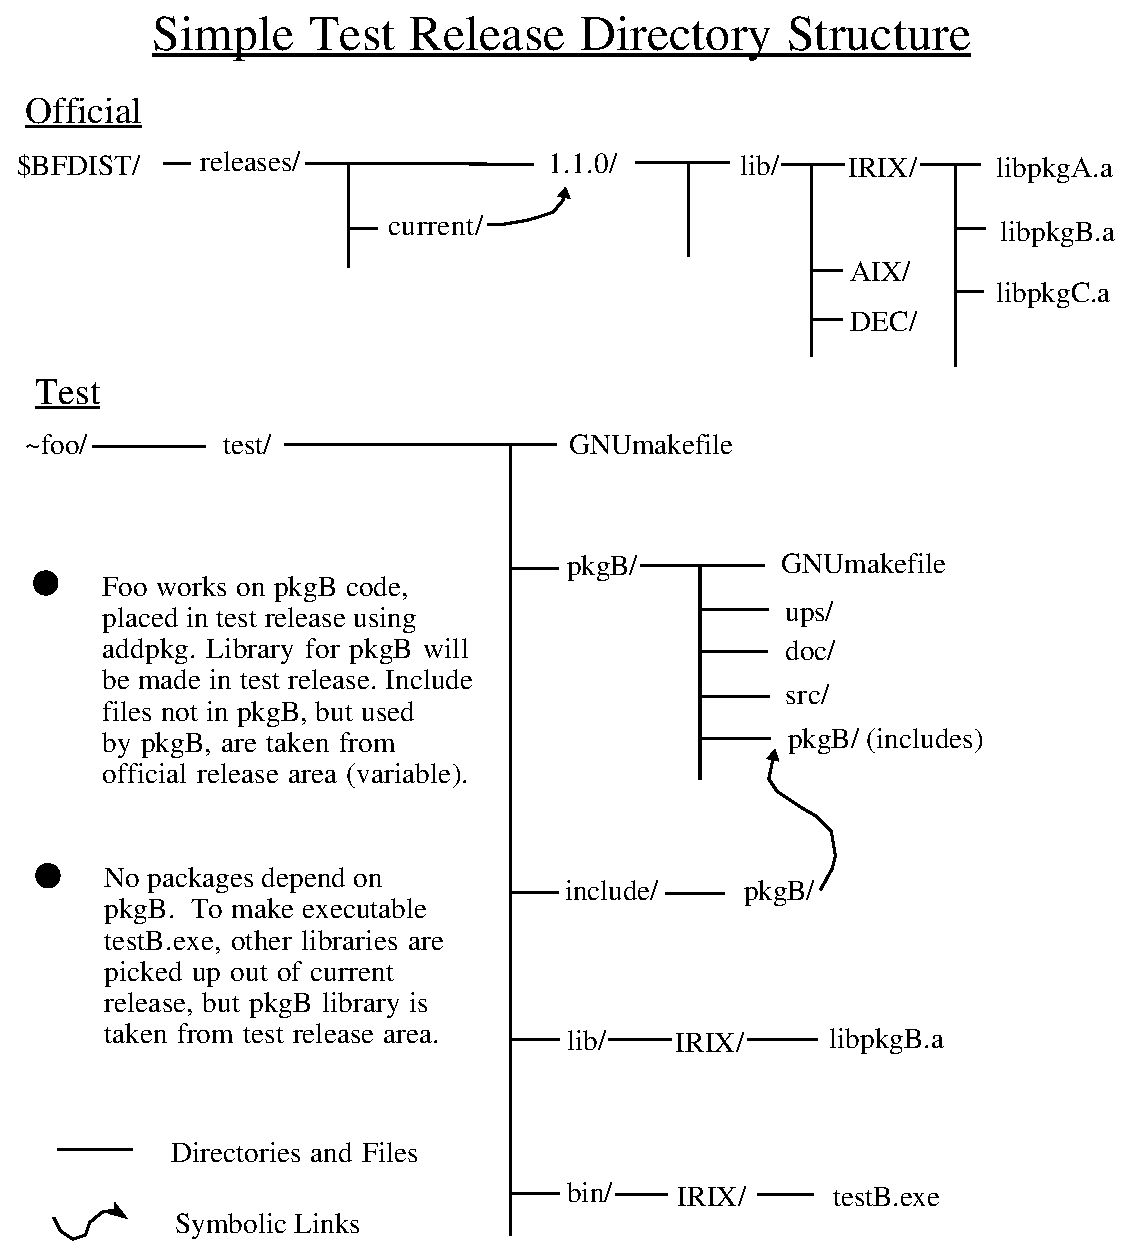
\includegraphics[width=5in]{run_2_dev_simple.eps}}
\caption[Simple Test Release Directory Structure]{ 
Diagram of a simple test release directory structure, and how it relates to the
official release directory structure.  Here the package ``pkgB'' is being
developed\index{packages!development of}, but since nothing else depends on pkgB, all other include files
\index{dependencies!simple test release} 
and libraries are taken from the current official release.}
\label{fig_dev_simple}
\end{figure}
\clearpage 

\vspace*{1.0in}
\begin{figure}[bht!]
%\epsfysize=8in
%\epsffile[36 54 581 756]{run_2_development.ps}
%\centerline{\epsfig{figure=run_2_development.eps,width=5in}}
\centerline{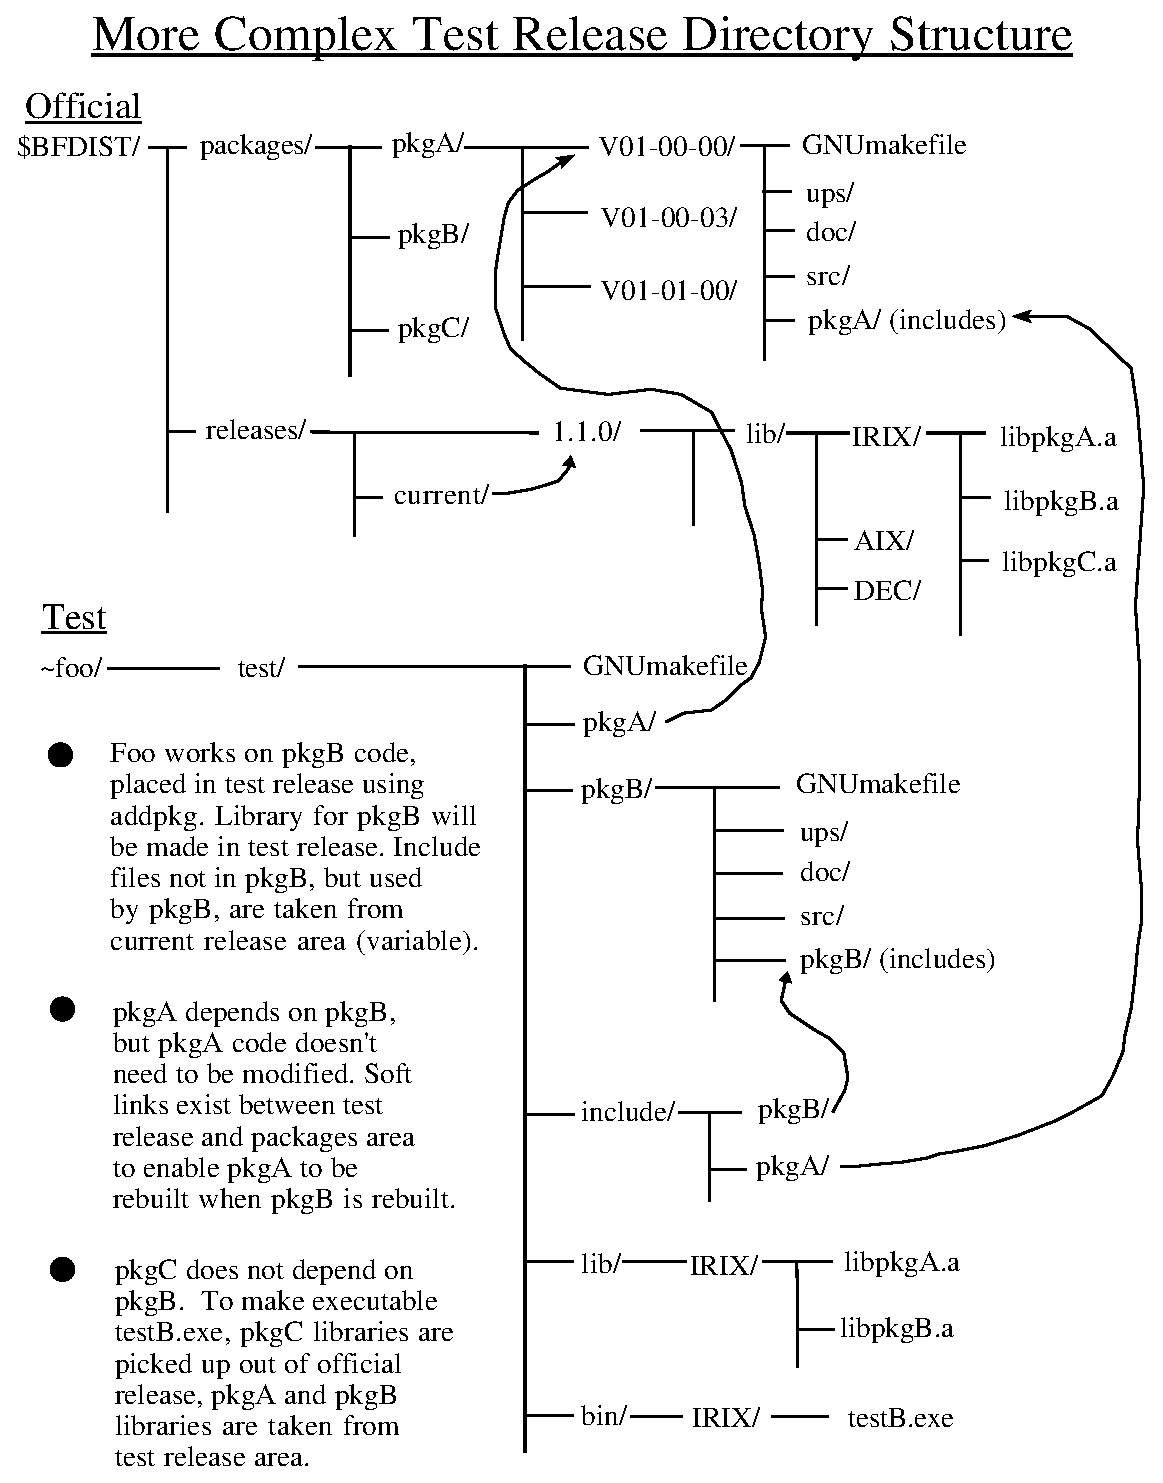
\includegraphics[width=5in]{run_2_development.eps}}
\caption[Complex Test Release Directory Structure]{ 
Diagram of a complex test release directory structure, and how it relates to the
official release directory structure.  Here the package ``pkgB'' is being
developed\index{packages!development of} , and ``pkgA'' depends on the contents of ```pkgB''. The curved lines 
\index{dependencies!complex test release} 
correspond to soft links.}
\index{soft links}
\label{fig_testrel}
\end{figure}
\clearpage 

\subsection{Distribution}
Initial distribution of the offical release structure to a remote machine will 
eventually be done via UPD once we have fully integrated it into our system.
In the meantime, we have developed simple scripts to 
initially distribute the release structure to a remote machine, 
discussed in Appendix~\ref{app_dist}.  
The release structure, those directories and soft links underneath
\index{soft links}
\$SRT\_DIST/releases in Fig.~\ref{fig_directory}, are saved in a tar file on the
server\index{client-server} machine.  
In addition, each package\index{packages!tar files}  is saved in it's own tar file. 
The location of the tarfiles on the distribution server\index{client-server} 
machines is given in ???
The
remote manager uses UPD, or currently the shell scripts described in 
Appendix~\ref{app_dist}, to copy these tar files from the distribution machine
to the remote machine and unwind them into the official 
releases\index{releases!area}  and packages\index{packages!area} 
area.  The tar file of the release specifies the flavor of the operating system and 
the version of the release. The user sets up the release using UPS as 
\index{UPS}
described in Section~\ref{sec_setup}.  The philososphy of using UPS with the
system is discussed in Appendix~\ref{app_ups}.

Once the remote machine has received an initial distribute of an official 
release, linking and development can take place. 
Distribution of the source code to a remote machine for user development is
accomplshed via SoftRelTools.  As described in section~\ref{sec_debug}, 
addpkg\index{addpkg} 
is used to checkout a complete package from CVS\index{CVS} for user development 
of that package\index{packages}. Within a test release, developers can
build and link code with their changes.  Libraries and include files from
other packages are taken from the official release. A development
release, described in section~\ref{sec_development}, can be constructed on 
any node and the code can be updated daily via CVS and rebuilt.  This is a
simple way of distributing the code to remote institutions on a daily basis,
and insuring that it works there just as well as on a central system. For
instructions on distribution of the development release at CDF, please see
section~\ref{sec_distribution_development}.

In summary, distribution of binaries and code of official 
releases\index{releases} takes place 
with UPD, after which users can link, and developers can work 
\index{linking!and distribution}
on packages  distributed to their test release by SoftRelTools.

%================================================================================
% All the appendices
%================================================================================

\clearpage
{\Huge \flushleft Appendix}
\appendix

%%%%%%%%%%%%%%%%%%%%%%%%%%%%%%%%%%%%%%%%%%%%%%%%%%%%%%%%%%%%%%%%%%%%%%%%%%%
% CVS
%%%%%%%%%%%%%%%%%%%%%%%%%%%%%%%%%%%%%%%%%%%%%%%%%%%%%%%%%%%%%%%%%%%%%%%%%%%
\section{Appendix on Version Control with CVS}
\label{app_cvs}

Concurrent Versions System (CVS)\index{CVS!introduction} is a 
freeware version control system that is widely
used by freeware developers including those in high energy physics. 
It is used by the CERN and Fermilab computing
divisions and by the following physics collaborations: ATLAS, CMS, SDSS, NuTeV,
CLEO, and BaBar.  Now it is also being used by CDF, D0 and BTeV. 
\index{BaBar}
\index{CDF}
\index{D0}
\index{BTeV}

Additional information can be found at:

\begin{itemize}
\item CVS Documentation <http://www.fnal.gov/docs/products/cvs>
\item CVSH <http://www.fnal.gov/cd/FUE/cvsh/>      
\end{itemize}

\subsection{ The CVS Repository and Basic Concepts}
\index{CVS!introduction|(}

CVS\index{CVS!repository} extends the notion of revision control from
a collection of files in a single directory, as in CMS, to a hierarchical
collection of directories each containing revision controlled files.
For example, two CVS\index{CVS!repository} repositories designed to contain the CDF offline software
\index{CDF}
\index{CDF!repositories}
are shown in Fig.~\ref{fig_repository}.      


\begin{figure}[tbh]
\begin{center}
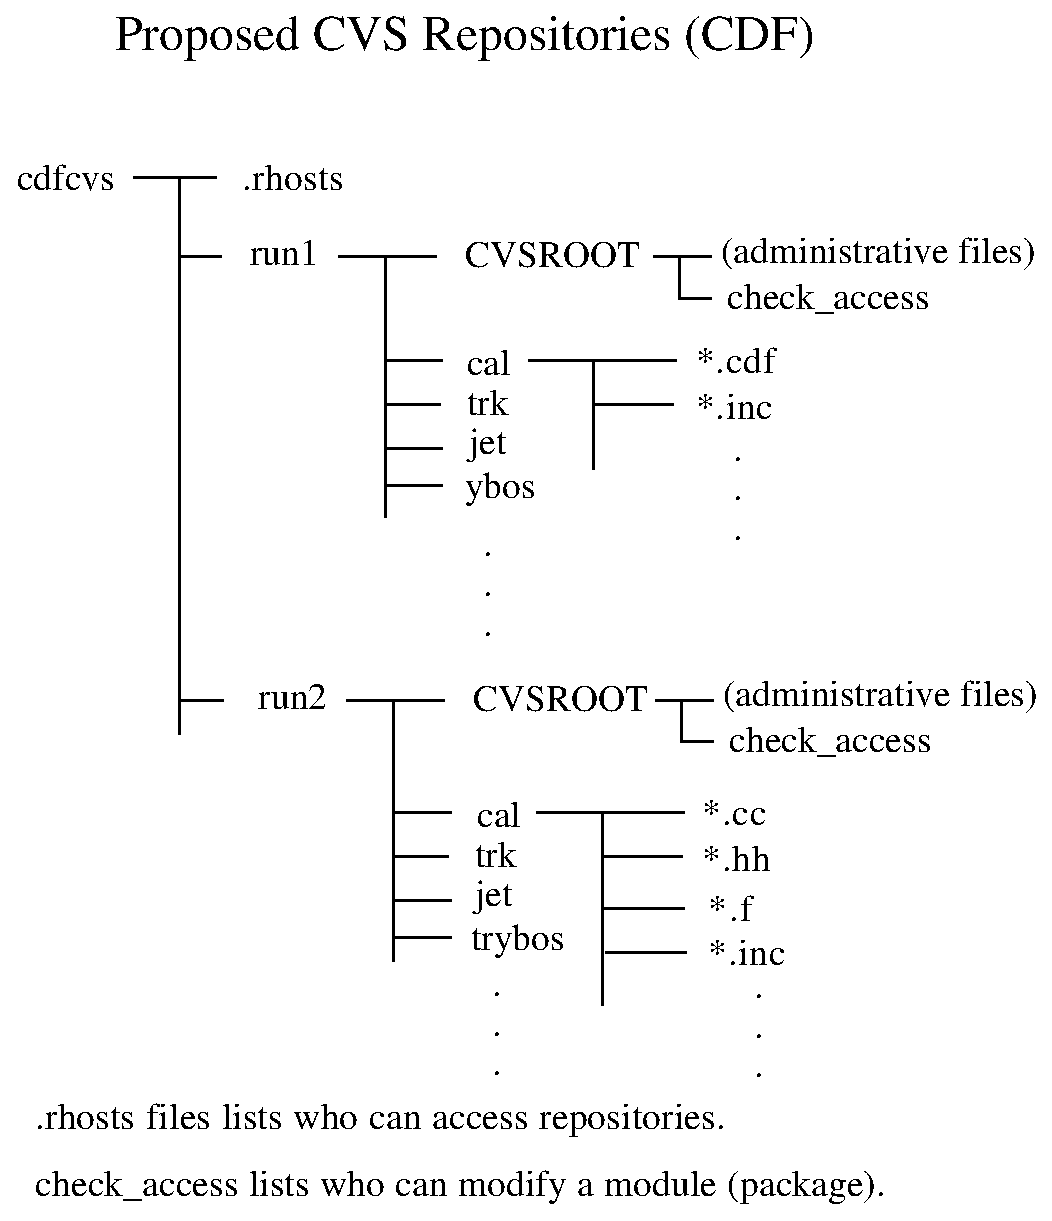
\includegraphics[width=4.0in]{two_repositories.eps}
\end{center}   

%\vspace*{-0.5in}
\caption[CVS Repositories]{
The structure of two CVS\index{CVS!repository} repositories, one for run 1 and one
for run 2.}
\label{fig_repository}
\end{figure}

Like CMS groups, CVS\index{CVS!module} collects files together into {\em modules}, and allows
operations on entire modules.  For example, the jet library would be a
module. Like a CMS class, CVS\index{CVS}
allows a collection of specific file versions to have a name, called a
{\em tag}.  CVS\index{CVS!file versions} labels each file with version
numbers, and allows branches and merging as depicted in Fig.~\ref{fig_branch}.
\begin{figure}[tbh]
\begin{center}
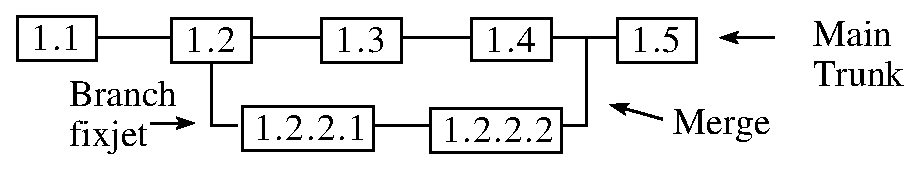
\includegraphics[width=6in]{cvs_revisions.eps}
\end{center}
\caption[Revisions, Branching and Merging]{
The versions of a particular file along the main trunk of the revision,
1.1, 1.2, 1.3, 1.4 and 1.5 are shown, along with a branch called {\ttfamily
fixjet},
that consists of modifying revision 1.2 into 1.2.2.1 and 1.2.2.2.  The
branch was merged back into the main trunk after revision 1.4 was complete,
giving revision 1.5.}
\label{fig_branch}
\end{figure}
As its name indicates, CVS\index{CVS!concurrent development} encourages concurrent revision by multiple
developers in parallel, unlike CMS which is designed for linear revision of
reserved files.  A script has been written to allow the command {\ttfamily
reserve} in CVS\index{CVS!reserve script} if desired.

\subsection{ Basic CVS Commands: A Single Revision Cycle}

As an example for the CVS\index{CVS!revision cycle} novice, the following commands perform a single
software revision cycle:
\begin{quote}
\ttfamily
cvs checkout jet/jtc90s.F\index{CVS!commands!checkout} \\
cd jet \\
cvs log jtc90s.F\index{CVS!commands!log} \\
emacs jtc90s.F \\
cvs commit -m "Changed jet energy scale!" jtc90s.F\index{CVS!commands!commit} \\
cd .. \\
cvs release -d jet \index{CVS!commands!release}\\
\end{quote}
The {\ttfamily cvs checkout}\index{CVS!commands!checkout} command creates in the users working directory a
subdirectory \texttt{jet/}, and places in \texttt{jet/} the file
\texttt{jtc90s.F}. This is like {\ttfamily CMS fetch} with an additional directory structure
created. The user goes to the \texttt{jet/} subdirectory and issues the
{\ttfamily cvs log} command\index{CVS!commands!log}, which presents her with the history of the file
\texttt{jtc90s.F}, like {\ttfamily CMS history}. The user then edits the file
(in this case using \texttt{emacs}) and places the file
back in CVS using {\ttfamily cvs commit}\index{CVS!commands!commit} and including comments, like
{\ttfamily CMS replace/keep}.  Finally the user passes back up to the working
directory and removes the entire jet/ directory tree with the command
{\ttfamily cvs release -d}\index{CVS!commands!release}, which checks to make sure there aren't any changes  
left to incorporate before deleting the files.
\index{CVS}
\index{CVS!introduction|)}

%%%%%%%%%%%%%%%%%%%%%%%%%%%%%%%%%%%%%%%%%%%%%%%%%%%%%%%%%%%%%%%%%%%%%%%%%%%
% Structure
%%%%%%%%%%%%%%%%%%%%%%%%%%%%%%%%%%%%%%%%%%%%%%%%%%%%%%%%%%%%%%%%%%%%%%%%%%%
\clearpage
\section{Appendix on the SRT Software Release Directory Structure}
\label{app_structure}

    To accommodate the storage of the various components of such a release, 
a consistent tree-structured hierarchy of directories is established. 
For expository purposes, we identify each directory with its depth (distance 
from the base) in the hierarchy. All quoted file names correspond to the 
labels in Figure~\ref{fig_directory}.

\subsection{The root directory (depth 0)}

    At the base (root) of this hierarchy is a single directory. Labelled 
``\$SRT\_DIST/'', this directory's sole purpose is to provide a starting point for 
the structure. In this root directory are entries for (the directories at the 
roots of) the two major subtrees of the structure, ``packages/''
\index{packages!area} 
 and ``releases/"\index{releases!area}. 

\subsection{The ``packages/'' directory (depth 1)}

    This directory serves as a root for the source code, documentation, 
makefiles, etc., for all versions of all packages in the product. Thus, each 
entry in ``packages/''\index{packages!area} is the starting point for a particular package. Note 
carefully that only items from the CVS\index{CVS!repository} repository are found. 

\subsubsection{Package directories ``pkgA/'', ``pkgB/'', ... (depth 2)}

    Each of these directories, direct descendents of ``packages/''
\index{packages!area} , serves as the
root of all the code, etc., associated with all versions of a single package. 
These directory names typically match the corresponding CVS\index{CVS!module} module name. Each 
such directory will have as many entries as the package has versions. 

\subsubsection{Individual version directories ``V01-00-00/", ... (depth 3)}
\label{sec_version}

    Each distinct version of a given package has its own root directory, a 
direct descendent of the package's root at depth 2 described above. The name 
of a version directory typically matches the release tag associated with the 
corresponding versions of the files in the CVS\index{CVS!tag or version} repository. 

\subsubsection{Depth 4 and beyond}
\label{sec_depth4}

    At this level, we find the source structure corresponding to (directly 
descended from the version root of) a particular version of a particular 
package. Among these entries, we might typically find: 
\begin{enumerate}
\item ``GNUmakefile'' (for the complete package)\index{packages!GNUmakefile} , 
\item  ``ups/'' (directory holding setup and unsetup files).
\index{UPS!subdirectory}
\item ``doc/'' (directory for tutorial and other documentary files), 
\item ``man/'' (directory to contain Unix-style man pages), 
\item ``src/'' (directory containing .cc and .f files), 
\item ``include/'' (directory holding .h and .inc files), 
\end{enumerate}

    Note: Figure~\ref{fig_directory} does not show all these directories, but 
they are clearly implied by the accompanying narrative. Also, 
Figure~\ref{fig_directory} labels the ``include/'' directory with the 
package name; however, this name is not a requirement of the structure but one which we 
recommend. This is because it reflects the including convention adopted in
the code: \#include pkgname/incname (see section~\ref{sec_include}).  

Recall that binary files are not intended to be located here.
However, one could conceive of additional directories here, such as ``test/'' or 
``examples/'' or ``tools/'', not necessarily part of all packages.

    The guiding principle is that, at this level, the logical structure of a 
package ought to dictate the directory structure. For reasons to become clear 
shortly, the ``include/'' directory is required, and must contain all those 
files that are visible to, and hence may be included by, any other packages or 
user software. 

The Unix-style man pages are put in the ``man/'' area of the directory 
structure. The UPS project setup file modifies the users MANPATH to include 
\index{UPS!MANPATH}
this area.

\subsection{The ``releases/'' directory (depth 1)}

    This direct descendent of the product root directory serves as a base for 
all vetted releases of the product. Each entry in this directory is the 
starting point for one such release. 

\subsubsection{Individual release directories ``1.0.0/", ... (depth 2)}

    Each of these directories, direct descendents of ``releases/", serves as the
root of all the information needed to make use of a release of the entire 
product. The name of a release directory typically matches the identification 
of a release in terms of the collection of all sources. 

    In addition, there are two standard directory names found at this level: 
``production/'' and ``current/''. These are only links to other release 
\index{soft links}
directories. They serve, however, as convenient and standardized labels so 
that users need not necessarily be cognizant of new releases: as each new 
release is installed, these directory links are intended to be broken and 
re-created as appropriate.\index{releases!soft links}

    At this level a general makefile can be created automatically to build the 
entire release tree. The makefile will simply: 
\begin{itemize}
\item invoke each of the package-specific makefiles\index{packages!GNUmakefile}  
(previously described) in turn, and 

\item install the resulting libraries and binaries into the respective 
``lib/'' and ``bin/'' flavor-specific subdirectories. 
\end{itemize}
\paragraph{\underline{Release component package directories ``pkgA/", ... (depth 3)}}

    Each of these directories corresponds to one of the 
packages\index{packages}  that make up 
the release, reflected by their parent directory, of the product. These 
directories are named for their corresponding packages. 

    However, in order to reduce unnecessary duplication of information already 
present within the ``packages/'' substructure, each of these directories is 
simply a link to the directory (at depth 3, described in 
\index{packages!soft links} 
\index{soft links}
section~\ref{sec_version} above) corresponding to the appropriate version of 
the package used to construct this release. 

\subsubsection{The ``include/'' directory (depth 3) and its descendents}
\label{sec_include}

    The intent of this directory, also a direct descendent of an individual 
release directory, is to serve as the indirect base for all .h files that 
are intended to be visible to any user of the software product. 

    This ``include/'' directory contains links, named for the individual 
\index{soft links}
\index{packages!soft links} 
packages, to the various depth 4 ``include/'' directories found under the 
``packages/'' structure (described among section~\ref{sec_depth4} above). In 
this way, code duplication is avoided, yet all include files are accessible to 
the user from one convenient source. 

The convention for including files in the source code is
 \#include pkgname/incname.
Here an 
include file, incname, is associated with a unique package, pkgname, necessary 
if two packages\index{packages!include files} have different include files with the same name.      

\subsubsection{The ``lib/'' and ``bin/'' directories (depth 3)}

    Via these directories, the remaining direct descendents of an individual 
release directory, we find a path to the software product's binaries. As is 
traditional, executables are found under ``bin/", while user-linkable libraries 
\index{linking!library locations}
are found under ``lib/". 

\subsubsection{Flavors directories ``IRIX/", ``AIX/'', ... (depth 4)}
\label{app_flavors}

\begin{sloppypar}
    These directories come into play when the software product is supported on
multiple platforms. When such is the case, ``bin/flavor/'' would serve to 
consolidate all executables for a given platform, while ``lib/flavor/'' would 
play a similar role for user-visible libraries. 
The directory is actually given a name that is a concatenation of the flavor
and version of the operating system, for example IRIX5 instead of IRIX.
This name (e.g. IRIX5) is stored in the environmental variable \$SRT\_ARCH.
\end{sloppypar}

\subsection{Usage of the directories}

    In the following sections we explain how the SRT directory structure and 
its Software Release Tools are envisioned to relate to the various client 
communities that deal with them. 

\subsubsection{A user's viewpoint}

    The UPS setup of a particular release sets the user's path, manpath, etc., 
\index{UPS!MANPATH}
\index{UPS!PATH}
in such a way that binaries are directly accessible, include files can be 
available through an environment variable pointing to the release ``include/'' 
tree, and the libraries can be used by a reference to the library tree 
environment variable via the ``-L'' compiler option. 
\index{compiler!options}

    The directory structure assumes that most users will make use of a complete
release, rather than mixing-and-matching packages across releases. If, however, 
a user would like to work with release ``A'' of a product but use version ``B'' of 
a package ``pkgC'', s/he should use the SRT ``newrel'' command to recreate the 
\index{newrel!users viewpoint}
release structure in his/her own working directory. To this command the user 
has to specify version ``B'' of package ``pkgC''. Version ``B'' of pkgC needs to 
be built in this new test release context. The user can then link his/her own 
\index{linking}
executable against this new test release. 

\begin{sloppypar}
Those users who want to write their own scripts and makefiles just need to 
know a few things. As discussed in section~\ref{sec_setup}, the UPS setup 
\index{UPS!SRT\_DIST and SRT\_CURRENT}
\index{UPS!environment}
defines the environmental variables \texttt{SRT\_DIST} and \texttt{SRT\_CURRENT}.  
The environmental variable \texttt{SRT\_ARCH} is also defined to indicate the flavor 
of operating system, as discussed in appendix~\ref{app_flavors}. In principal,
these are the only environment variables you need to use the software release 
structure. Although we strongly recommend the use of our setups and makefiles, 
the user is free to suitably define these variables to point at the right areas,
and then write their own scripts and makefiles.  The user needs to know 
that compilation with package include files\index{packages!include files}  is 
accomplished using the compilation option 
\texttt{-I\$SRT\_DIST/releases/\$SRT\_CURRENT/include}, and linking with package
\index{linking!-L option}
libraries is accomplished using the link option 
\texttt{-L\$SRT\_DIST/releases/\$SRT\_CURRENT/lib/\$SRT\_ARCH}. Users who 
prefer to do it themselves should be able to use this information to write 
their own sripts and makefiles.  However, we recommend that the provided
scripts and makefiles be used.
\end{sloppypar}

\subsubsection{A developer/contributor's viewpoint}

    In a private ``workdir'' directory, using the command ``newrel'' the developer 
\index{newrel!from developers viewpoint}
can recreate the release structure starting from a reference release. 
To modify an existing package,  the contributor can use the ``addpkg''
\index{addpkg!from developers viewpoint} command 
that checks out the module from the CVS\index{CVS!repository} repository. 
The checkout command creates the main directory structure for the package 
reflecting the module organization in CVS. Extra directories need to be 
created by the package-specific make file. The developer then 
communicates changes to the librarian, who commits them to CVS\index{CVS}.

\subsubsection{A librarian/package manager's viewpoint}

\begin{sloppypar}
    A librarian has to go through the same steps a developer goes through, but 
he has write access to the CVS\index{CVS} repository for his own 
package\index{packages!librarian}. The librarian has access to the package-specific directory in the 
\$SRT\_DIST/packages tree. This can be accomplished via a group uid, and 
trusted developers can be added or removed from this uid using the systools
commands \texttt{cmd addmember} and \texttt{cmd delmember}.
\end{sloppypar}

\subsubsection{A product/configuration manager's viewpoint}

    The product manager has write access to the entire \$SRT\_DIST tree. He can 
operate directly in the \$SRT\_DIST directories and use the ``-p'' (production) 
option of the ``newrel'' command. 
\index{newrel!managers viewpoint}

%==========================
% UPS and SRT
%==========================
\section{Appendix Using UPS with SRT}
\index{UPS}
\label{app_ups}
 
First some general comments. It is important to note that much of the 
information about which package\index{packages} 
    version works with what other package version, is contained in the release 
directory structure itself. This
    removes the requirement that this information be stored in the UPS database
\index{UPS!databases}
as dependencies. This is
\index{dependencies!UPS}
    desirable for a number of reasons. Maintaining and distributing this 
information in the form of the UPS 
    database has through the years proven to be difficult. Various recent 
additions to UPS help - cups is an
\index{UPS}
    example - but it is still true that you must be a UPS expert in order to 
\index{UPS}
effectively maintain this information. In
    a period of stable code distributions this is not a disaster; however, in a 
heavy development period it may
    become one. The other reason for minimizing UPS's knowledge of package 
\index{packages!UPS}\index{UPS}
dependencies is that it will
\index{dependencies!UPS}
    speed up and simplify the process of setting up a set of packages.
\index{packages!setup}  There 
will be fewer ambiguities about
    which versions of packages actually get setup. 

    However the concept of UPS product dependencies is still needed. There are 
\index{dependencies!UPS}
many products that we use, over
    which we have little or no control. In fact any 
package for which we do not keep
    our own CVS\index{CVS!external packages} library, would be classified in this category. Let's call 
them external packages\index{packages!external}. Examples
    would be products like cernlib or tcl/TK. These packages do not live in the 
directory structure,
    and therefore the older mechanisms for handling dependencies are still required. 
\index{UPS}
\index{dependencies!UPS}
Hopefully the coupling between
    this class of packages\index{packages!inderdependencies}  is not strong. For instance, no one would be happy if
you could only use version A of
    tcl/Tk with version B of cernlib. Also, note that references to libraries and 
binaries from this class of package are still referred to through environmental 
variables or path setting. They are not copied to the
 \verb|$SRT\_DIST/release/<version>/lib| or \verb|$SRT\_ROOT/release/<version>/bin| areas. 

\subsection{Using UPS for packages}
\index{packages!UPS} 
\index{packages!setup} 
\index{UPS!package setup}
\index{UPS}

    Packages inside the directory structure still need to be able to 
specify how environment variables,
    needed for the running of their package, must be set. For example, in the 
news product, NNTPSERVER
    must be set to the site news server machine; for tex, TEXINPUTS defines the
search list of directories to
    look for tex files. Many of the other uses of ups/setup.* files, like path 
\index{UPS}
modifying, are not needed by this type
    of package because all of the binaries live in the release structure. 
Therefore, for each
    package in the package tree, at the same level as doc, src, include and 
GNUmakefile, there is a UPS 
\index{UPS!subdirectory}
    subdirectory, which contains setup and unsetup files that are 
fragments of the
full project setup. These fragments are concatenated into the full setup 
and unsetup files in the release tree during the release build. 
Each of the fragments is a fast
equivalent of \texttt{setup <pkg>} with the appropriate version number.

\subsection{Using UPS with releases}
\index{UPS!release setup}

    In the release tree there is a UPS subdirectory at the same level as 
\index{UPS!subdirectory}
bin, lib, and include. It 
    contains a setup file that sets the path to contain the bin area of the
release and define anything else
    needed for the global release. 
From now on we refer to a global release
as a project. Thus a project is a set of experiment written products that 
get linked together into executables, and hence would form a release.  For
example online and offline could be separate projects.

The setup and unsetup file also have copied into them the 
fragments from all of the packages\index{packages!setup fragments} 
    contained in the release. These files could be built by the script that 
makes new releases\index{releases} (newrel), but currently they are build by the release 
manager by declaring the release of the project to UPS.  Marc Mengel has 
\index{UPS}
developed a utility called
\index{newrel!ups}
UPS\_COMPILE which we use to collect the fragments together into a 
\index{packages!UPS compile} 
\index{UPS!compile}
single script. The setup file
    also declares this release to the experiment UPS database so that users of 
\index{UPS!databases}
the release could say, for example, ``setup $<$project$>$ 
[$<$project-version$>$]'', as is done in section~\ref{sec_setup}.
At this time any external package dependencies could be
\index{dependencies!UPS}
defined in the UPS database.

\subsection{External Packages and UPS}
\index{packages!external} 
Not all packages used by the experiment will be included in the release 
structure. External packages, such as CERNLIB or tcl/TK or gcc, for which we 
do not usually rebuild the code, are not located in the release structure.  
They are located somewhere else which is pointed to by the normal UPS 
\index{UPS!external packages}
environmental variable.  We do not use CVS\index{CVS!external packages} to track the source code of external 
packages. There is no restriction on where the environmental variable 
\texttt{<product>\_DIR} points. If we need to rebuild external packages, we
use their own makefiles, not the SoftRelTools makefiles.

In the SoftRelTools makefiles we use the UPS \texttt{<product>\_DIR} 
\index{UPS!product variable}
environmental variables
\index{packages!external!environmental variables} 
to pickup external package libraries and include areas necessary for building.
These environmental variables may be defined through UPD dependencies, whereby
\index{dependencies!UPS}
we have declared the project to depend on a given version of an external 
package. The intent is that \texttt{<product>\_DIR} is set when we setup the
project, not via a separate ``setup $<$product$>$'' statement which might 
pickup the wrong version of the external product for the project.

%%%%%%%%%%%%%%%%%%%%%%%%%%%%%%%%%%%%%%%%%%%%%%%%%%%%%%%%%%%%%%%%%%%%%%%%%%%
% Makefiles
%%%%%%%%%%%%%%%%%%%%%%%%%%%%%%%%%%%%%%%%%%%%%%%%%%%%%%%%%%%%%%%%%%%%%%%%%%%
\section{Appendix on Makefiles in Software Release Tools}
\label{app_make}

SoftRelTools use GNU Make for building libraries and executables.
\index{gmake}
\index{gmake!GNUmakefile!user run2}
The file GNUmakefile, in the area where the gmake command
is given, tells GNU Make what to build.
%The user only needs to use
%the makefile in section~\ref{app_user_make} to link a job, and shouldn't need
%to modify it.
\index{linking}
The developer introducing a new package, or the user trying to link an
executable, needs to modify simple
makefiles described in section~\ref{app_package_make}.  Developers, code
librarians, and code managers will want to be aware of the
makefiles discussed in section~\ref{app_release_make}, but should
not need to modify them.   

\subsection{Package Makefiles}
\label{app_package_make}
\index{packages!GNUmakefile}
The following example of package makefiles, \\
\$SRT\_DIST/releases/\$SRT\_CURRENT/Framework/GNUmakefile 
and \\ \$SRT\_DIST/releases/\$SRT\_CURRENT/Framework/src/GNUmakefile, 
are used for building the libraries and executables of the Framework package.
\index{gmake}
\index{gmake!GNUmakefile!package level}
They are examples of typical package makefiles used by gmake in the examples of 
section ~\ref{sec_debug} and ~\ref{sec_newrel}. 
The first makefile only points gmake at the subdirectory src in which the
\index{gmake}
second makefile resides. The second makefile specifies the library target 
libapp.a, and includes the architecture specific makefile for the tcl package, 
on which the framework package depends.  Both makefiles include standard.mk 
which defines the compilation and dependency generation in detail.
\index{BaBar}
\begin{footnotesize}
\begin{verbatim}
$SRT\_DIST/releases/$SRT\SRT\__CURRENT/Framework/GNUmakefile 
# GNUmakefile for the BaBar Framework package
#
# uses SoftRelTools/standard.mk
#
#    Bob Jacobsen, Jan 96
#
#############################################################
# file lists (standard names, local contents)

# include file products
INC =

# library product
LIB =

#library contents
LIBFFILES  =
LIBCFILES  =
LIBCCFILES =

# subdirectories
SUBDIRS = src

# binary products
BINS =

############################################################
include SoftRelTools/standard.mk
\end{verbatim}
\end{footnotesize}
\vspace*{1in}
\begin{footnotesize}
\begin{verbatim}
$SRT_DIST/releases/current/Framework/src/GNUmakefile 
# new Makefile for Framework - the old one is unchanged.
#
# uses SoftRelTools/standard.mk
#
#############################################################
# file lists (standard names, local contents)

# include file products
INC =

# library product
LIB = libapp.a

#library contents
LIBCFILES  =
LIBCCFILES := $(shell ls *.cc)


# binary products
BINS =

# APPMain.o is required for Solaris link
all:
lib: $(libdir)/APPMain.o
$(libdir)/APPMain.o: $(libdir)/$(LIB)
        cd $(libdir); ar x $(LIB) APPMain.o
include SoftRelTools/arch_spec_Tcl.mk

############################################################
include SoftRelTools/standard.mk
\end{verbatim}
\end{footnotesize}


\subsection{Release, Standard, and Architecture Specific Makefiles}
\label{app_release_make}
At the top of every release is a GNUmakefile as shown in 
Fig.~\ref{fig_directory},~\ref{fig_dev_simple}, and ~\ref{fig_testrel}. The 
release makefile recognizes the experiment by 
means of the .experiment file, which contains names like CDF or D0. The release
\index{CDF}
\index{CDF!.experiment file}
\index{D0}
\index{D0!.experiment file}
\index{.experiment file}
makefile specifies what areas will be searched for include files when
compiling, and what areas will be searched for libraries when linking.
\index{linking}
Most important, for the library and executable targets, this file effectively 
loops over the individual package makefiles and runs make for them.
The release makefile is the heart of the building system.

The user makefiles and package makefiles described in the last section
includes the makefile standard.mk.  This makefile contains standard target 
definitions and rules for compilation and linking.  Similarly, standard.mk
\index{linking}
includes the file arch\_spec.mk, which contains the architecture specific
rules for each machine and operating system.
\clearpage



\clearpage
\addcontentsline{toc}{section}{References}
\begin{thebibliography}{99}

\bibitem{ref_sdss} CVS at SDSS is described on the Code Management WWW pages
at http://www-cdf.fnal.gov/offline/code\_management/sdss.html.
\index{CVS!SDSS-CVS}

\bibitem{ref_babar1} Bob Jacobsen, ``The BaBar Software Release Structure'',
\index{BaBar}
March 5, 1995, on the WWW at
http://www.slac.stanford.edu/BFROOT/dist/releases/current/SoftRelTools/ 
SoftRelToolIntro.ps.

\bibitem{ref_babar2} Bob Jacobsen, ``Using the BaBar Software Release 
Structure'', October 28, 1995, 
http://www.slac.stanford.edu/BFROOT/doc/Computing/Reconstruction/Notes/
SoftRelToolUser.ps.

\bibitem{ref_tuura} Lassi A. Tuura, ``Helper programs for Moose Directory
Structure'', http://wwwcn1.cern.ch/l/lat/www/notes/soft/dist/scripts.html.

\bibitem{ref_commentary} Walter Brown, Flavia Donno-Raffaelli and Elizabeth
Sexton-Kennedy, ``On the Software Release Directory Structure'' on the Code
Management WWW pages at 
at http://www-cdf.fnal.gov/offline/code\_management/srt.html.

\bibitem{ref_REBUILD} Flavia Donno-Raffaelli, ``REBUILD Users Guide and
Reference Manual'', CDF Note 1611, August 15, 1994.  Available on the WWW at
http://www-cdf.fnal.gov/offline/code\_management/rebuild.mem.

\bibitem{ref_cmgt_c++} See discussion of C++ implications on Code Management
\index{C++}
pages on the WWW at 
http://www-cdf.fnal.gov/offline/code\_management/c++.html.

\bibitem{ref_cvs} Basic information on cvs is available from the man pages 
and at http://fnnews.fnal.gov/cd/UNIX/cvs/cvs.html. The complete manual can
be obtained from http://www.loria.fr/$\sim$molli/cgi-bin/wilma.cgi/doc.
\index{CVS!references}.  A hardcopy of this manual is available in the CDF 
trailers office 149-E.

\bibitem{ref_cyclic} Information on Cyclic Software is available at 
http://www.cyclic.com/.

\bibitem{ref_uaf} ``UNIX at Fermilab'', Computing Division Document GU0001, 
available on the WWW at
http://www.fnal.gov/docs/UNIX/unix\_at\_fermilab/welcome.html

\bibitem{ref_alan} Alan Jonckheere, ``Configuration Management: A Turnkey 
System'', on the WWW at 
http://d0www.fnal.gov/\texttt{~}jonckheere/cmgt/turnkey.html

\bibitem{ref_dcd} Mathew Wicks, ``Fermi UNIX Environment DCD Products User
Guide'', DCD0003, DCD User Guide 3.4, January 19, 1993.

\bibitem{ref_cmgt_draft} ``Run 2 Code Management Report'', by Configuration 
Management Working Group on July 12, 1996, available on the WWW at 
http://fnpspa.fnal.gov/Run2/document.html.
\end{thebibliography}

%Index Cross References
\index{dependency files|see {.d files}} 
\index{deleting|see {removing}}
\index{get ! package|see {addpkg}}
\index{get ! test release|see {newrel}}
\index{information!about release|see {statusrel}}
\index{information!about repository|see {lscvs}}
\index{link ! symbolic|see {soft links}}
\index{link ! soft|see {soft links}}
\index{packages!installing production|see {newver}}
\index{packages!removing production|see {rmver}}
\index{packages!creating release|see {newrel}}
\index{packages!interdependencies|see {depend}}
\index{packages!soft links|see {lnkpkg}}
\index{packages!getting|see {addpkg}}
\index{packages!removing release|see {rmrel}}
\index{release!listing contents|see {statusrel}}
\index{release!creating|see {newrel}}
\index{release!removing see {rmrel}}
\index{removing!releases|see {rmrel}}
\index{removing!packages|see {rmver}}
\index{new ! production package|see {newver}}
\index{soft links!creating|see {lnkpkg}}
\index{compile!UPS |see {UPS}}
\index{UPS!dependencies|see {dependencies|UPS}}
\index{server|see {client-server}}
\index{linking!executable filename|see {EXENAME}}
\index{linking!.opt filename|see {OPTFILE}}
\index{make|see {gmake}}
\index{preprocessor|see {CPP}}
\index{version!control|see {CVS}}

\clearpage
\addcontentsline{toc}{section}{Index}
\documentclass[12pt]{article}
\usepackage{graphicx}
\topmargin -1in
\textwidth 6.5in
\textheight 9.5 in
\oddsidemargin 0.0in
\evensidemargin 0.0in
\baselineskip 14pt
\makeindex
\def\see#1#2{{\em see\/} #1}
\begin{document}
\begin{flushright}
\vspace*{0.5in}
CDF Note: CDF/DOC/COMP\_UPG/PUBLIC/3891 \\
\index{CDF}
D0 Note: 3118f \\
\index{D0}
Computing Division Note: GU0013 \\
\end{flushright}
\vspace{0.5in}
\begin{center}
{\LARGE SoftRelTools User's Guide}\\
\vspace{.5in}
{\large Version 2.0}\\
{\large \today }\\
\vspace{.5in}
{\large Last edited by Margaret Votava}\\
{\large \em Fermilab Computing Division}\\
\vspace{.5in}
{\large for:\\
Dave Adams, Jim Amundson, Jim Bellinger, Walter Brown, Glenn Cooper, 
Flavia Donno-Raffaelli, Lynn Garren, 
Herb Greenlee, Robert Harris, Alan Jonckheere, Robert Kennedy, Arthur Kreymer, 
Qizhong Li, Don Petravick, Ruth Pordes, Lars Rasmussen, 
Elizabeth Sexton-Kennedy, Scott Snyder and Gordon Watts.}
\vspace{.5in}
\end{center}
\begin{abstract}
This is the user's guide for the Fermilab version of Software Release Tools, 
a UNIX based software management system for large, collaborative projects
that is used by several experiments at Fermilab.
The system provides software version control with CVS\index{CVS} 
configured in a client-server\index{client-server} mode.
For management and 
building we have adopted the directory structure and SoftRelTools originally 
developed by the BaBar collaboration. 
The system handles the 
version control, management, building, and distribution of code written in 
Fortran, C and C++. A distinguishing feature of the system is its
\index{C++}
ability to allow rapid asynchronous development of 
package versions, 
which can be easily integrated into complete consistent
releases\index{releases} of the entire offline software.  This 
has reduced the time it takes for new and modified code to be made available to 
users. 
\end{abstract}

\clearpage
\tableofcontents
\listoffigures
\listoftables

\clearpage
\section{Introduction}

This document is the User's Guide for SoftRelTools (SRT). It is meant
to give an overview of the SRT environment and commands
from a code developers point
of view. Code librarians should refer to the SRT Reference Guide for
more detailed explanation of the SRT configuration parameters and commands. 

SRT is very flexible in the style in which it allows developers to operate. 
This flexibility presents a difficulty in writing a general purpose "how to"
User's Guide because each librarian has imposed a cycle that is most 
appropriate for that particular release and a naming convention that
best suits the cycle. Users should refer to the specific instructions 
for a given release for the naming conventions and the development cycle. 

Release specific instructions can be found at:
\begin{itemize}
\item CDF Run 2
\item D0 Run 2
\item SDSS
\item ZOOM
\item BTeV http://www-btev.fnal.gov/internal\_documents/code/code\_management.html
\item Minos 
\end{itemize}

\subsection{What is SRT}

SoftRelTools (SRT) is a toolset for managing large software projects, aka releases,
that consists of smaller units, aka packages, that are developed in parallel
by a diverse programming community. It allows individual developers to 
work on their package independently of the ongoing work in other packages,
and to update the whole project when they are satisfied with their 
modifications. In this way, the developer is responsible for the management
of his individual package, while the release librarian is responsible for 
management of the all the packages as a whole.


\subsection{How to use this document}
This document has been written in the style of a book, or pedagogical users
manual, with discussion and illustrations.  People seeking a general 
overview of the system may want to read the normal sections, omitting the 
appendices.  New users or developers who want to do something with the system 
quickly, and don't want to read much, are advised to follow the examples in 
section~\ref{sec_examples} and Appendix~\ref{app_build}. Those seeking a 
reference manual for answering arbitrary questions about the system will find
it quickest to use the index at the back of the document.  

\subsection{Other light reading}

For sleepless nights:
\begin{itemize}
\item SRT Reference Guide
\item CVS User's Guide http://www.fnal.gov/docs/products/cvs/
\item gmake User's Guide http://www.fnal.gov/docs/products/gtools/make.1.html
\item Barbar SRT document
\item CVSH http://www.fnal.gov/cd/FUE/cvsh/ 
\end{itemize}

\section{Software Release Structure}
The software release structure provides a flexible and easy to use
framework for both releasing and developing code.  Code is typically grouped
into {\em packages}\index{packages!definition}; however, it is essential to have a {\em release} of all 
code in 
all packages. The structure must support simultaneously both
releases\index{releases} of stable versions of the 
packages\index{packages}, and asynchronous development of 
the individual packages themselves.  This is in contrast to a structure which
is oriented solely along the lines of a release, where package versions
are only stamped with the release number. The BaBar software release
\index{BaBar}
structure~\cite{ref_babar1,ref_babar2}, which supports both
asynchronous development of packages\index{packages!asynchronous development} 
and grouping packages\index{packages} into 
releases\index{releases!definition},
is shown in Fig.~\ref{fig_directory}. A commentary on this structure with 
a detailed verbal description of Fig.~\ref{fig_directory} is given in 
Appendix~\ref{app_commentary}.

The environmental variable {\ttfamily \$SRT\_DIST} is used as a root to add flexibility.  
Below it are found separate subtrees for packages\index{packages} and releases\index{releases}. 
Within the
package subtree, each package can contain one or more different {\em versions}.
This allows the package librarians to develop packages 
asynchronously\index{packages!asynchronous development},
and assign the package a version number when the package is ready for use
by others.  Within the release subtree, there is a subdirectory for each
existing release.  A release directory consists of soft links to a set of 
\index{soft links}
consistent package versions, plus the libraries and binaries created from
the release for various machine architectures.  Again, the release manager
can use this to create releases\index{releases} as required.  Links within the release
\index{soft links}
directory can be used to provide default names for particular releases, for
example ``current'' for the release recommended for general use at the present
time.

Notice that the soft links between releases\index{releases!soft links} and 
packages\index{packages!soft links} are
\index{soft links}
to the source code only; the libraries and binaries are native to the release.
This is necessary because in C++ a change to a header file used by package A can
\index{C++}
affect the result in package B which uses package A, even if package B does 
not use the part of the header file that is changed or added.  Unlike common
blocks in Fortran, where you can add to the end of a common block which is
used by many packages\index{packages} and you do not need to recompile all the code, in C++
\index{compile}
\index{C++}
if you modify a header file you have to recompile all the code that depends on 
\index{dependencies!and C++} 
that header file. The only way to insure consistent results when
changing a header file is to rebuild both libraries.  

\begin{figure}[tbh]
%\centerline{\epsfig{figure=run_2_directory.eps,width=4.5in}}
\begin{center}
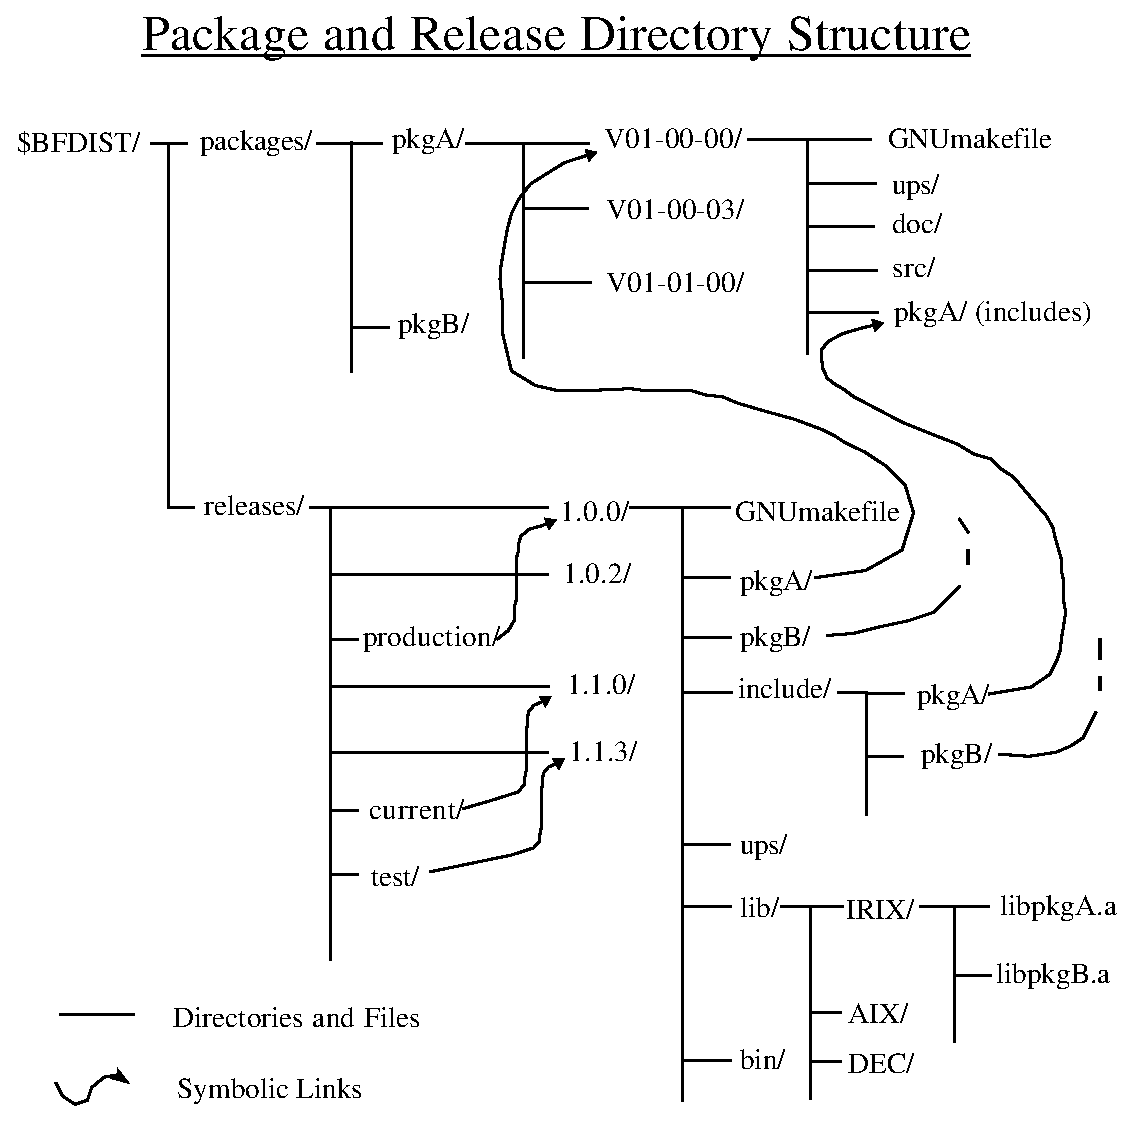
\includegraphics[width=4.5in]{run_2_directory.eps}
\end{center}
\caption[Official Release Directory Structure]{ 
Diagram of the directory structure.  This example includes two
packages: 
``pkgA'' and ``pkgB''\index{packages!definition}\index{packages!figure}. 
The curved lines correspond to soft links\index{soft links} between 
releases\index{releases!definition}\index{releases!figure} and packages.}
\label{fig_directory}
\end{figure}

\subsection{Package and Release Versions and Labels}
\index{version!of package}
\index{version!numbering convention}
The package and release numbering system is designed to allow multiple versions
of packages\index{packages!numbering} and many releases\index{releases!numbering} of code to be available to the collaboration.

The convention for package version numbers is Vxx-yy-zz where
xx is the major version field, yy the minor field, and zz is a bug fix
field incremented for small changes. This version number is also the 
CVS\index{CVS!tag or version} tag of 
that version. The first version is then V00-00-00.
The code manager will install this tag on the initial version of
the code in the repository, and either librarians or the code manager can tag 
subsequent versions using the CVS\index{CVS!commands!rtag} command rtag.

The convention for releases\index{releases!numbering} is x.y.z, where x is the 
major release number\index{releases!major},
y the minor release\index{releases!major}, and z is a bug fix 
number\index{releases!bug-fix}. Thus 1.0.0 would be a major
release that is rigorously tested,  1.1.0 would be a minor release based on 
1.0.0 and would require less testing, and 1.1.3 would be a bug fix or fast 
release based on 1.1.0 and might have almost no testing.  The ``production''
release would generally be a symbolic link to a major release, like 1.0.0.
\index{soft links}
The ``current'' release could be a minor release, like 1.1.0. The ``test'' release 
could be bug fix release, such as 1.1.3.  There could be many major, minor,
and bug fix releases\index{releases!bug-fix}, and only a few of them might have symbolic links pointing
\index{soft links}
to them with names like ``production'', ``current'', ``test'',
``fast-tracking'', etc.
This labelling system allows many different releases, and the level of
validation\index{releases!validation} is apparent from the number.

\subsection{Development Releases}
\label{sec_development}

\index{development} 
In addition to frozen releases with specific versions, SRT structure
also supports a more dynamic development environment. A development release is 
not required, but it is a very useful option for integration, bug detection,
and access to the most recent available code. Most often, 
developers are making changes on different packages in parallel. At
various stages during this development, they will want to share there
work with others. Making a frozen release for each of these stages
would consume a lot of disk space in addition to being a code librarian's
nightmare. 

In Fig.~\ref{fig_development_release} we show the structure of a development
release, which is nearly identical to a frozen release.  The difference is that
the soft links all point to the ``development'' version of the package in the
packages area.  The development version of the package was checked out of
CVS when the package was first added to development, and every day the 
development version is updated via a {\ttfamily cvs update} command. The 
{\ttfamily cvs update} command is a convenient way of distributing 
development, sending only the code that has changed from the repository to the 
development release.  Since we use client-server cvs, all nodes in the system 
are equal, and the process of getting development on a central system is no 
different than the process of getting development anywhere.  Note that no
development actually takes place in the development package area. Developers
are required to develop code in their test releases (see next section) and check
that code back in to the repository, so that the code can propogate to all
development nodes everywhere. 

\begin{figure}[tbh]
%\hspace*{0.1in}
%\epsfysize=6in
%\epsffile[36 100 581 674]{development_release.ps}
%\centerline{\epsfig{figure=development_release.eps,width=4.5in}}
\centerline{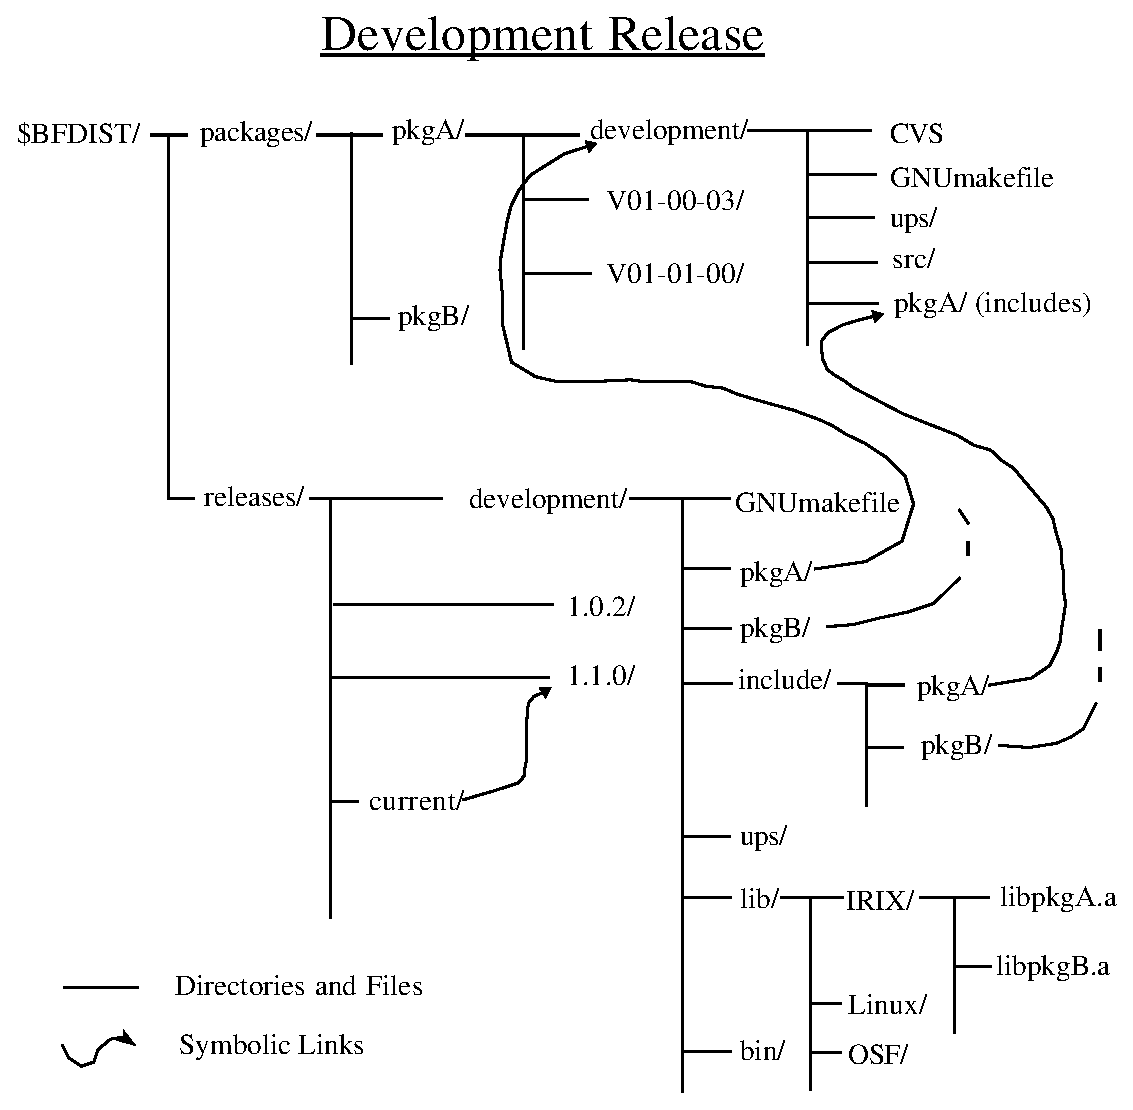
\includegraphics[width=4.5in]{development_release.eps}}
\vspace*{-0.5in}
\caption[Development Release Directory Structure]{ 
Same as Fig.~\ref{fig_directory} except the release called development
contains soft links to the development version of each package, which is 
checked out from CVS and updated from the main repository. There is nothing
hardwired about the tag "development", and each environment may have a 
different term. Please check the specific instructions from your code 
librarian.}
\label{fig_development_release}
\end{figure}

\index{development!update} 
At some interval on each development node 
{\ttfamily cvs update} is done for each package in the release, and 
then the release is rebuilt with the command {\ttfamily gmake}. At
CDF this happens every morning. Developers
can then use the development release to link against.  

A facility exists in 
SoftRelTools to scan the log files that result from the build,
find compilation and linking errors, and send error reports to the designated
developers and package librarians.  
\index{development!error reporting} 
This provides developers with immediate
feedback, and errors are caught and fixed quickly.  
This SoftRelTools error\_reporter facility
also can create error status tables, like the on in Fig.~\ref{fig_status_table}.
Ask your code librarian for links to the location of these log files. 

Although naive users may want to use a frozen release, for stability, 
in a rapidly developing software environment, developers need to use 
the development release to insure that their additions really work with
the most recent software.  

\begin{figure}[tbh]
%\centerline{\epsfig{figure=status_table.eps,width=4.5in}}
\centerline{\includegraphics[width=4.5in]{status_table.eps}}
\vspace*{-4.7in}
\caption[Status Table for Development Release]{ 
Example summary of errors detected during one night's build of the 
Run 2 development 
software at CDF. The lib stage is the compilation stage of the package,and 
the bin stage is the compilation and linking of executables for that package.
A text entry in the table indicates there was an error for the package 
indicated. Here for example there was an error linking an executable in the
TrackingMods package under Linux using the KAI compiler, and no errors 
anywhere else. This summary was generated on Wed Jul 22 08:00:19 1998 by the
error\_reporter facility in SoftRelTools.}
\label{fig_status_table}
\end{figure}

\subsection{Using the Software Release Structure}
\label{sec_examples}

This section will describe the overall procedures needed to develop
in an SRT environment.  In short, a user wants to develop a certain
package. He needs to define a context, or base release, in which this 
package will be compiled and linked. He must define a "test" release
in some working area, then copy the package to be modified
into this working area, and finally set symbolic links for header files
and libraries to the other packages in the base release - see Figure ???. 

The user is afforded many options to globally describe his development 
environment. One of which is a "super" test release. 
Look at figure ???. The default SRT behavior is to define
the path for header files to include both directories in the test 
release as well as the base release. If a user deleted a header file from 
package B in the test release, the make files would still find it in the
base release. This can lead to some confusion. SRT supports the concept
of a "super" test release which will only look for include files in the
test release. It does this by creating a directory called "super" in the
test release and putting links to each pacagke's header files therein. 


The SoftRelTools commands themselves are defined in more
detail in Section ~\ref{sec_commands}. 
Once again, you should
refer to your code librarian's instructions for the naming conventions and
practices unique to your specific configuration. Section~\ref{sec_setup}
describes how to setup SoftRelTools, necessary before any SRT 
commands can be executed.
Section~\ref{sec_debug}                                
describes constructing a test release using {\ttfamily newrel} \index{newrel} 
for development
of a package obtained using {\ttfamily addpkg}.\index{addpkg}  
This is also how a user links a job.
Section~\ref{sec_newver} describes making the new package version official 
using {\ttfamily newver}\index{newver}. Section~\ref{sec_newrel} describes making a new
production release, including the new package version, using {\ttfamily newrel}.

\subsubsection{Setup}
\label{sec_setup}
Because it is flexible and each distribution has opted for different
features, setting up the environment is the most confusing part of using 
SRT. The user needs to work out of a test release. If he doesn't already have
one, he needs to create one with the SRT "newrel" command. This only needs
to be done once, and the user can work from the this area indefinitely. 
Additionally, the user needs to run srt\_setup in each shell that his wishes
to develop in, ie, each time he logs in or creates an xterm. There is a bit
of a chicken and egg problem here in that some srt\_setup switches require that
a test release already have been created (e.g., -A), but you can't create the 
test
release until srt\_setup has been run. The solution is to execute srt\_setup
twice. 

Note that the user can have more than one test release and switch between 
them, but this is not recommended for the novice SRT user. An additional note
is that if you have if you have done an srt\_setup -A and switch test 
releases, you need to run srt\_setup again. 

SRT is very loosely coupled with UPS. It has no requirements on UPS itself,
but is modelled after it. Certain environment variables must be defined, 
e.g., ??? SRT\_DIST in a global file and then srt\_setup run. Code librarians
have wrapped this distribution specific scripts. 
Again, check with your code librarian for your specific instructons. 

For example, below are
the Run 2 setup commands at CDF and D0 (for a more complete list see ???
\index{CDF}
\index{CDF!setup}
\index{D0}
\index{D0!setup}
):
\begin{enumerate}
\item {\ttfamily source /d0library/d0local.login }\\
{\ttfamily setup D0RunII [<base-release>]}\\
\index{D0}
This will setup the D0 Run II software.  
\item {\ttfamily source $\sim$cdfsoft/cdf2.cshrc}\\
{\ttfamily setup cdfsoft2 [<base-release>]}\\
This will setup the CDF Run II software. \\
\end{enumerate}

where the files \texttt{d0local.login} and 
\texttt{cdf2.cshrc} define the UPS databases for D0 and CDF in Run II:
\index{UPS!databases}
\index{CDF}
\index{CDF!UPS databases}
\index{D0}
\index{D0!UPS databases}
the appropriate file can either be sourced 
interactively or in the users \texttt{.login} file.  


How does it know SRT\_DIST???
The setup commands define the  SoftRelTools enviromental variables 
\texttt{SRT\_DIST}, \texttt{SRT\_BASE\_RELEASE}, and \texttt{SRT\_ARCH}. 
\texttt{SRT\_DIST} is the
main directory, \texttt{SRT\_BASE\_RELEASE} is the release 
identifying name
or number in the \texttt{\$SRT\_DIST/releases} directory, and \texttt{SRT\_ARCH} 
specifies the UNIX operating system type and version number.
\texttt{<base-release>} is an optional
argument specifying the release, and if absent will default to the current
release. Note that \texttt{SRT\_BASE\_RELEASE} is not
a pathname.  For example, the \texttt{SRT\_BASE\_RELEASE} release would be found at
\texttt{\$SRT\_DIST/releases/\$SRT\_BASE\_RELEASE}, so \texttt{SRT\_BASE\_RELEASE} could be a name 
like ``current'' or
a number like ``1.0.4''.  In addition, if using in a UPS environment, it 
defines a convenient 
\index{UPS!project variable}
environmental variable (\texttt{<project>\_DIR}, which is 
\texttt{CDFSOFT2\_DIR}, \texttt{D0RUNII\_DIR}, etc.) which 
points at the area \texttt{\$SRT\_DIST/releases/\$SRT\_BASE\_RELEASE}. 
Libraries and include 
files from packages\index{packages} will be taken from the \texttt{<project>\_DIR} area, 
when linking and compiling, unless another area is specified 
by a test release (see section~\ref{sec_debug}). 

\subsubsection{Creating a test release}
\label{sec_testrel}

As previously stated, the user needs to create a working area in which
to make his changes. This is called a test release and is created with
the SRT command newrel.  This command need only be executed once per
test release directory. 

Once the test release is created, the user needs to populate it 
with the particular packages he wishes to modify via the lnkpkg command. 
Let's say that header files in a second package depend on the package the
user wants to modify. The user will want to build the libraries in 
the second package, but not modify the code. He can add the second package
to the test release via the lnkpkg command. 

\begin{itemize}
\item {\ttfamily cd <wherever>}\\
      For example, in Figs.~\ref{fig_dev_simple} and ~\ref{fig_testrel},
the user typed {\ttfamily \verb|cd ~foo|}.
\item {\ttfamily newrel -t <base-release> <new-release>} \\
\index{newrel!general use by developers}
     The "-t" switch is required and tells newrel that this is a developer's
working area and NOT a new official release to be created in \$SRT\_DIST. 
<base-release> is the official release to work off from. In many cases,
this is development. <new-release> is the arbitrary string that you
define to be your working directory. 
For example, in Figs.~\ref{fig_dev_simple} and ~\ref{fig_testrel},
the developer typed {\ttfamily newrel -t current test}.

This created the {\ttfamily test} directory and populated it with the main 
GNUmakefile and empty sub-directories include, lib, and bin, etc.  
It did not
create the {\ttfamily pkgA} or {\ttfamily pkgB} directories.
The release number 
\texttt{<base-release>} is written to a file \texttt{.current}, used by 
\texttt{GNUmakefile} to determine which production release to use.
\item {\ttfamily cd <new-release>} \\
For example, in Figs.~\ref{fig_dev_simple} and ~\ref{fig_testrel},
the user typed {\ttfamily cd test}.
\item {\ttfamily srt\_super\_init } \\
	This is an optional command that should be executed if the user
wants super test functionality. 


\item {\ttfamily addpkg [-h] <package> [<tag>]}\\
\index{addpkg!general use by developers}
This checks out the package from CVS\index{CVS!commands!checkout} to create the package sub-directory
and its contents. 
For example, in Figs.~\ref{fig_dev_simple} and ~\ref{fig_testrel},
the user typed {\ttfamily addpkg <pkgB>}.
\index{addpkg}
Note that this will check out of CVS\index{CVS!tag or version} the 
version of \texttt{<package>} that was used
to make the \texttt{<base-release>}.  This may not be the head version of the 
package,
however, it is a version that is garanteed to work with 
\texttt{<base-release>}.  If
the developer instead wants to modify the head version in CVS\index{CVS!tag or version} (the latest 
version along the main trunk), then the -h option must be used with addpkg.
\index{addpkg!-h option}
The developer should be aware that the head version is not guaranteed to 
work with the \texttt{<base-release>}.

If \texttt{<tag>} is present, {\ttfamily addpkg} does a 
{\ttfamily cvs checkout -r<tag> package}.  
\index{CVS!commands!checkout}
\index{CVS!tag or version}
\index{addpkg!tag or version argument} In
Figs.~\ref{fig_dev_simple} and ~\ref{fig_testrel}, the user typed 
{\ttfamily addpkg pkgB} \index{addpkg}
to create the sub-directory {\ttfamily pkgB} and fill
{\ttfamily pkgB} with sub-directories and code from CVS. {\ttfamily addpkg} 
\index{CVS}\index{addpkg!creates soft links}
also creates a soft link between the test release include area and the newly 
created package include area.  For example, in 
Figs.~\ref{fig_dev_simple} and ~\ref{fig_testrel}, {\ttfamily addpkg}
\index{addpkg!soft links}
created a symbolic link \verb|~foo/test/include/pkgB/| which points to
\verb|~foo/test/pkgB/include/|. 

In Fig.~\ref{fig_testrel} there is a package, {\ttfamily pkgA}, which 
depends on include files in {\ttfamily pkgB} that user Foo will modify.  
However, Foo does not need to modify any of the code in {\ttfamily pkgA}, 
Foo only wants to modify {\ttfamily pkgB}.  To allow Foo to rebuild the 
libraries for {\ttfamily pkgA} without checking out the code for {\ttfamily
pkgA}, we have created symbolic links between the test release and the
official packages\index{packages!soft links} area.  The symbolic link \verb|~foo/test/pkgA/| points to 
\$SRT\_DIST/packages/pkgA/1.1/, and the symbolic link 
\verb|~foo/test/include/pkgA/| points to \$SRT\_DIST/packages/pkgA/1.1/include/.  
The SoftRelTools script {\ttfamily lnkpkg} 
\index{lnkpkg}
creates these 
links between the test release area and the desired version of the package
(see Appendix~\ref{app_lnkpkg}). You can figure out which packages you need
to link to by running the SoftRelTools script \texttt{depend} 
\index{packages!interdependencies}
\index{depend}
\index{dependencies!depend script}
(see Appendix~\ref{app_depend}).      


Developers using the development release will {\bf always} want to use the
-h option to checkout the head: no other syntax will work.  
\index{development!addpkg} If you use the 
development release and type {\ttfamily addpkg pkgA}, then CVS will look
for a version of {\ttfamily pkgA} with the tag {\ttfamily development}, and
no such tag exists on the package, resulting in an error message.
The correct syntax is {\ttfamily addpkg -h pkgA}.
For frozen releases, if the -h option is not used, then a tagged version of the 
package\index{packages!tags} is 
being checked out, and has a CVS\index{CVS!sticky tag} "sticky tag" on it. The 
command 
\texttt{cvs update -A}\index{CVS!commands!update} must be 
performed before commiting the package back into the
repository (or else CVS\index{CVS!branch confusion} thinks you are trying to 
commit to a new branch and
complains). If you are adding new files to a package\index{packages!add files}, you should do a 
\texttt{cvs update -A}\index{CVS!commands!update} before doing a 
\texttt{cvs add}\index{CVS!commands!add}, or the files will be 
added to a branch off of the version checked out, not to the head.  If you 
mistakedly added the files to a branch, you should 
\texttt{cvs remove}\index{CVS!commands!remove} them, 
\texttt{cvs commit}\index{CVS!commands!commit} the remove, and do a 
\texttt{cvs update -A}\index{CVS!commands!update} before adding 
them again. To do a \texttt{cvs commit} you will need privileges: contact
your release manager.

Developers need to be aware that 
\texttt{cvs update -A}\index{CVS!commands!update} updates your area to
the head of CVS\index{CVS!head}, bringing in any changes that have been made 
to the head 
while you were working on the package.  CVS\index{CVS!informational codes} 
prints a code telling you which files were modified (M) by you, which files 
need
updating (U) in your area, and which files both need updating and there are
conflicts (C) between your changes and others which 
CVS\index{CVS!conflicts} asks you to resolve.
If there were conflicts CVS\index{CVS!conflicts!backups} creates a backup of 
the file prefixed by \#.
If this is too intimidating for you, 
first do a \texttt{cvs -n update -A}\index{CVS!commands!update} which will 
merely print the informational code, and will not change a single file in your 
area.  
\end{itemize}

\subsubsection{Compiling and linking for developers or users}
\label{sec_debug}
\index{linking}
\index{linking!for developers|(}

This method of compiling and linking is fully supported.
This is the procedure a developer will follow to work on one or more packages
as a unit.  End users who want to modify one or more packages for their own
purposes can also use this technique. The simplest example of the directory
structure is shown in Fig.~\ref{fig_dev_simple} and a more complex example is 
shown in Fig.~\ref{fig_testrel}.  In these figures Foo is developing code
for package {\ttfamily pkgB}.
\begin{itemize}

\item {\ttfamily cd <new-release>} \\
For example, in Figs.~\ref{fig_dev_simple} and ~\ref{fig_testrel},
the user typed {\ttfamily cd test}.

\index{gmake!for developers}
\index{gmake!in test release}
\item {\ttfamily gmake}\\
\index{gmake}
This will invoke GNU make to build the libraries (lib target) and 
executables (bin target) for each package in your test release. 
The individual package makefiles\index{packages!GNUmakefile} are discussed in
Appendix~\ref{app_package_make}. 
For example in Fig.~\ref{fig_dev_simple}, on a machine running IRIX, \texttt{gmake} 
created the test release library for pkgB, \verb|~foo/test/lib/IRIX/libpkgB.a|, 
and the test release executable for pkgB, \verb|~foo/test/bin/IRIX/testB.exe|. When
constructing libpkgB.a, all include files not in pkgB were taken from \\
\texttt{\$SRT\_DIST/releases/\$SRT\_BASE\_RELEASE/include/*}, and when constructing 
\verb|testB.exe| all libraries other
than libpkgB.a were taken from 
\texttt{\$SRT\_DIST/releases/\$SRT\_BASE\_RELEASE/lib/\$SRT\_ARCH}.  Similarly, in
Fig.~\ref{fig_testrel}, \texttt{gmake} created the test release library for
\index{gmake}
both pkgA and pkgB, and the test release executable for pgkB.  Once again,
all include files not in pgkA or pkgB were taken from 
\texttt{\$SRT\_DIST/releases/\$SRT\_BASE\_RELEASE/include/*}, and when constructing 
\texttt{testB.exe} all libraries other
than \texttt{libpkgB.a} and \texttt{libpkgA.a} were taken from 
\texttt{\$SRT\_DIST/releases/\$SRT\_BASE\_RELEASE/lib/\$SRT\_ARCH}.
However, gmake will look for header files and 
\index{gmake!and header files}
libraries in the \texttt{<base-release>}, found in the \texttt{.current} file, 
regardless of how the user has modified the environment via the setup command.
Thus the \texttt{SRT\_BASE\_RELEASE} variable is redefined by gmake
\index{gmake!SRT\_BASE\_RELEASE redefined}
\index{gmake}
based on the contents of the \texttt{.current} file, and this redefinition only last
for the duration of the \texttt{gmake} command.
\index{gmake}
\end{itemize}

In addition to established packages, the above steps can also be used to create 
your own package\index{packages!new}, or work area, and link it in with your test release.  If you 
are creating a new package called \texttt{work}, in place of \texttt{addpkg} 
\index{addpkg!new package}
you will want to do a \texttt{mkdir work}, and copy your source files to the 
\texttt{work} subdirectory.  In addition you will need to have 
a \texttt{GNUmakefile} similar to one that appears in the top directory of any 
of the packages.  In that GNUmakefile you will need to specify the library
name (where the object files go), and add this library to the list of libraries
looked for in any link. If you are linking an executable associated
with this work package, you will want to specify them in this GNUmakefile,
and give the link command.  For example, assume you have two files, \texttt{test2.F}
containing a program \texttt{test2}, and \texttt{test.F} containing a 
subroutine \texttt{test} which is called by \texttt{test2}.
You should make a library \texttt{libwork.a} to contain the compiled subroutine 
\index{compile}
\texttt{test}, and link it to the main program \texttt{test2}, by 
\index{linking}
adding the following lines to the package makefile specified in 
Appendix ~\ref{app_package_make}:
\begin{quote}
\ttfamily
LIB = libwork.a  \\
LIBFFILES  = \$(filter-out test2.F, \$(wildcard *.F))  \\
override LOADLIBES += -lwork                         \\ 
BINS = test2.exe                                     \\
\$(bindir)test2.exe: test2.F \$(LIBS)                \\
\hspace*{0.3in} echo linking test2 ; \$(FC) \$(FCFLAGS) \$(CPPFLAGS) \$(LDFLAGS) \verb+\+ \\
\hspace*{0.3in} -o \$@ \$< \$(LOADLIBES) \$(LDOUT);\\
\index{linking!command in makefile}
\end{quote} 
\index{CPP}
Here the first line specifies the the library as \texttt{libwork.a}. The 
second
line indicates that all Fortran files except \texttt{test2.F} (the main 
program) will go in
this library. Note that \texttt{test.F} is never mentioned explicitly, it is
simply picked up from the area and compiled because it has the suffix
\index{compile}
\texttt{.F}. The third line adds \texttt{libwork.a} to the list of libraries 
to be loaded.
The executable name \texttt{test2.exe} is specified in the fourth line.  The 
fifth line says
that the executable \texttt{test2.exe} depends on the main program file 
\texttt{test2.F} and the 
libraries.  The sixth and seventh line give the rule to make the executable
\texttt{test2.exe} (these lines are begun with a tab).  Developers can add 
similar lines to their GNUmakefile, to 
construct executables from their own packages.  If in doubt, copy from 
a GNUmakefile in an established package. When the new 
packages\index{packages!new} are fully
tested, they can be migrated to the release.
\index{linking!for developers|)}

\subsubsection{To put a new version of a package in the production area}
\label{sec_newver}

The developer changes a package and communicates those changes to the
package librarian. The librarian then commits the changes to the 
CVS\index{CVS}
repository. When the package librarian decides that it's time to make a 
new official version of the package, the librarian tags the consistent set of 
files that form the package with a unique CVS tag via the command 
{\ttfamily cvs rtag <version> <package>}\index{CVS!commands!rtag}. 
Once the version of the package has been tagged 
in the CVS\index{CVS} repository, then:
\begin{itemize}
\item {\ttfamily cd \$SRT\_DIST/packages/<package name>}
\item {\ttfamily newver -p <cvs tag name>}\\
\index{newver}
This creates the new version of the package\index{packages!new version}  in the official packages tree.  
The \texttt{<cvs tag name>} is the package version number, and has the format
\texttt{Vxx-xx-xx}, where \texttt{x} is between 0 and 9. The 
area you are in, {\ttfamily \$SRT\_DIST/packages/<package name>}, provides the
name of the package for the {\ttfamily newver} command.  The ``-p'' option 
is currently required, and indicates this is a production version, so the 
files will be write-protected and have their timestamps updated.
\texttt{newver} also declares this version of the product to the ups
database\index{UPS!databases}\index{UPS!declare}. 
\end{itemize}

\subsubsection{The develoment cycle before a new production release}
\label{sec_dev_cycle}
The previous two sections illustrate how the development cycle can take 
place before a new production release is created.  First, as discussed in
section~\ref{sec_debug}, developer Foo checks out and works on \texttt{pkgB}
in a test release. When \texttt{pkgB} works to Foo's satisfaction, Foo returns
the package\index{packages!development cycle}  to the \texttt{pkgB} libarian and requests that a new version of
the package be created.  Second, as discussed in section~\ref{sec_newver}, the
package\index{packages!librarian}  librarian commits the package back into CVS\index{CVS!tag or version}, tags it with a new 
version number, and creates a new version of the package in the official area
using \texttt{newver}.  This does not produce any object libraries, or a new
\index{newver}
release, which is the topic of the next section.  Third, Foo comunicates to
other developers that a new version of the package is available for testing
in the official area.  To get the new version of the package and test it, 
another developer need only follow the procedure in section~\ref{sec_debug},
checking out the specific version of the package that the librarian created
with Foo's changes.  To do this they would create a test release in their area
using \texttt{newrel -t <base-release> <new-release>}, 
\index{newrel!in development cycle} and then do a 
\texttt{lnkpkg pkgb <tag>} 
\index{lnkpkg!in development cycle}, 
or a \texttt{addpkg pkgB <tag>}
\index{addpkg!in development cycle}, 
\index{addpkg!tag or version argument}, 
where tag is the 
version number.  If there is 
a special \texttt{<base-release>} that Foo wants used in conjunction with 
\texttt{pkgB}, then Foo is obligated to inform the other developers.  Once 
enough people have used the new version of \texttt{pkgB}, and are happy with
it, the release manager should seriously consider making an official release
with it, so that developers will not need to produce object libraries
themselves in their test release.  This is the topic of the next section.

\subsubsection{To make a new production release with the package version 
just created}
\label{sec_newrel}
\index{newrel!production}
After one or more packages\index{packages}  have been updated, somebody decides that a release
incorporating the changes is required.
\begin{itemize}
\item {\ttfamily cd \$SRT\_DIST/releases}
\item {\ttfamily newrel -p <old release> <new release>}\\
The old release provides the list of packages\index{packages!old release} to include, and the initial 
libraries and executables. {\ttfamily newrel} will prompt for the version of
each package\index{packages!version}  required. 
\item {\ttfamily cd <new release>}
\item {\ttfamily ups declare -r <directory> -z <ups-database> -f <flavor> <project> <release>}
Here we declare the release to UPS, which establishes a UPS database entry for
the release. At CDF\index{CDF!UPS}, this command invokes a 
UPS\_COMPILE\index{UPS!compile} of all 
the products in the release thereby creating the script \texttt{comp\_setup}, 
which is invoked whenever the user types \texttt{setup cdfsoft2}. 
The arguments of \texttt{ups declare}\index{UPS!declare!release} we use are \texttt{<directory>}, the 
directory on disk where the release resides, \texttt{<ups-database>}, the
disk location of the ups database, \texttt{<flavor>}, the UNIX operating system 
type of the release's binaries (IRIX, AIX, etc.), \texttt{<project>}, the 
project name (cdfsoft2, D0RunII, etc.), and \texttt{<release>}, the release 
number.
\index{gmake!for production release}
\item {\ttfamily gmake}\\
\index{gmake}
These should be repeated for every supported architecture.  Errors that occur
at this stage may result in changes to one or more packages and the creation
of a new release, but should not be corrected by changing the source in this
release. After the release is made a soft link characterizing the release as
\texttt{current} or \texttt{development} may optionally be created in the
area \texttt{\$SRT\_DIST/releases} pointing to the release number.  If so, the
release manager needs to also declare~\index{UPS!declare} the release to UPS 
as \texttt{current} or \texttt{development} for consistency.
\end{itemize}

\begin{figure}[bht!]
%\epsfysize=8in
%\epsffile[36 120 576 756]{run_2_dev_simple.ps}
%\centerline{\epsfig{figure=run_2_dev_simple.eps,width=5in}}
\centerline{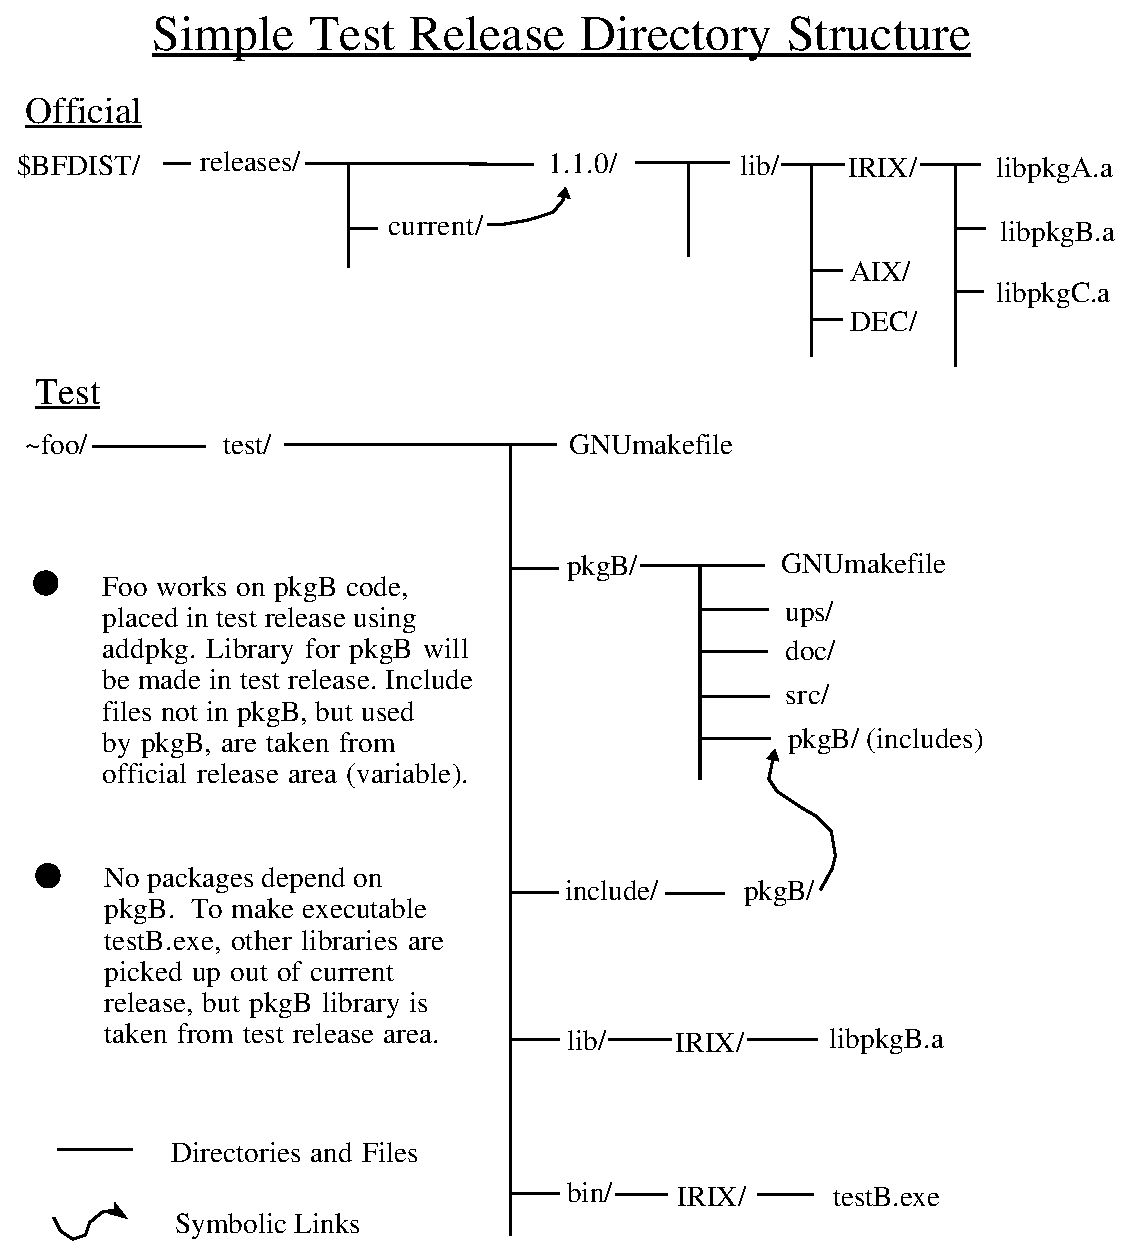
\includegraphics[width=5in]{run_2_dev_simple.eps}}
\caption[Simple Test Release Directory Structure]{ 
Diagram of a simple test release directory structure, and how it relates to the
official release directory structure.  Here the package ``pkgB'' is being
developed\index{packages!development of}, but since nothing else depends on pkgB, all other include files
\index{dependencies!simple test release} 
and libraries are taken from the current official release.}
\label{fig_dev_simple}
\end{figure}
\clearpage 

\vspace*{1.0in}
\begin{figure}[bht!]
%\epsfysize=8in
%\epsffile[36 54 581 756]{run_2_development.ps}
%\centerline{\epsfig{figure=run_2_development.eps,width=5in}}
\centerline{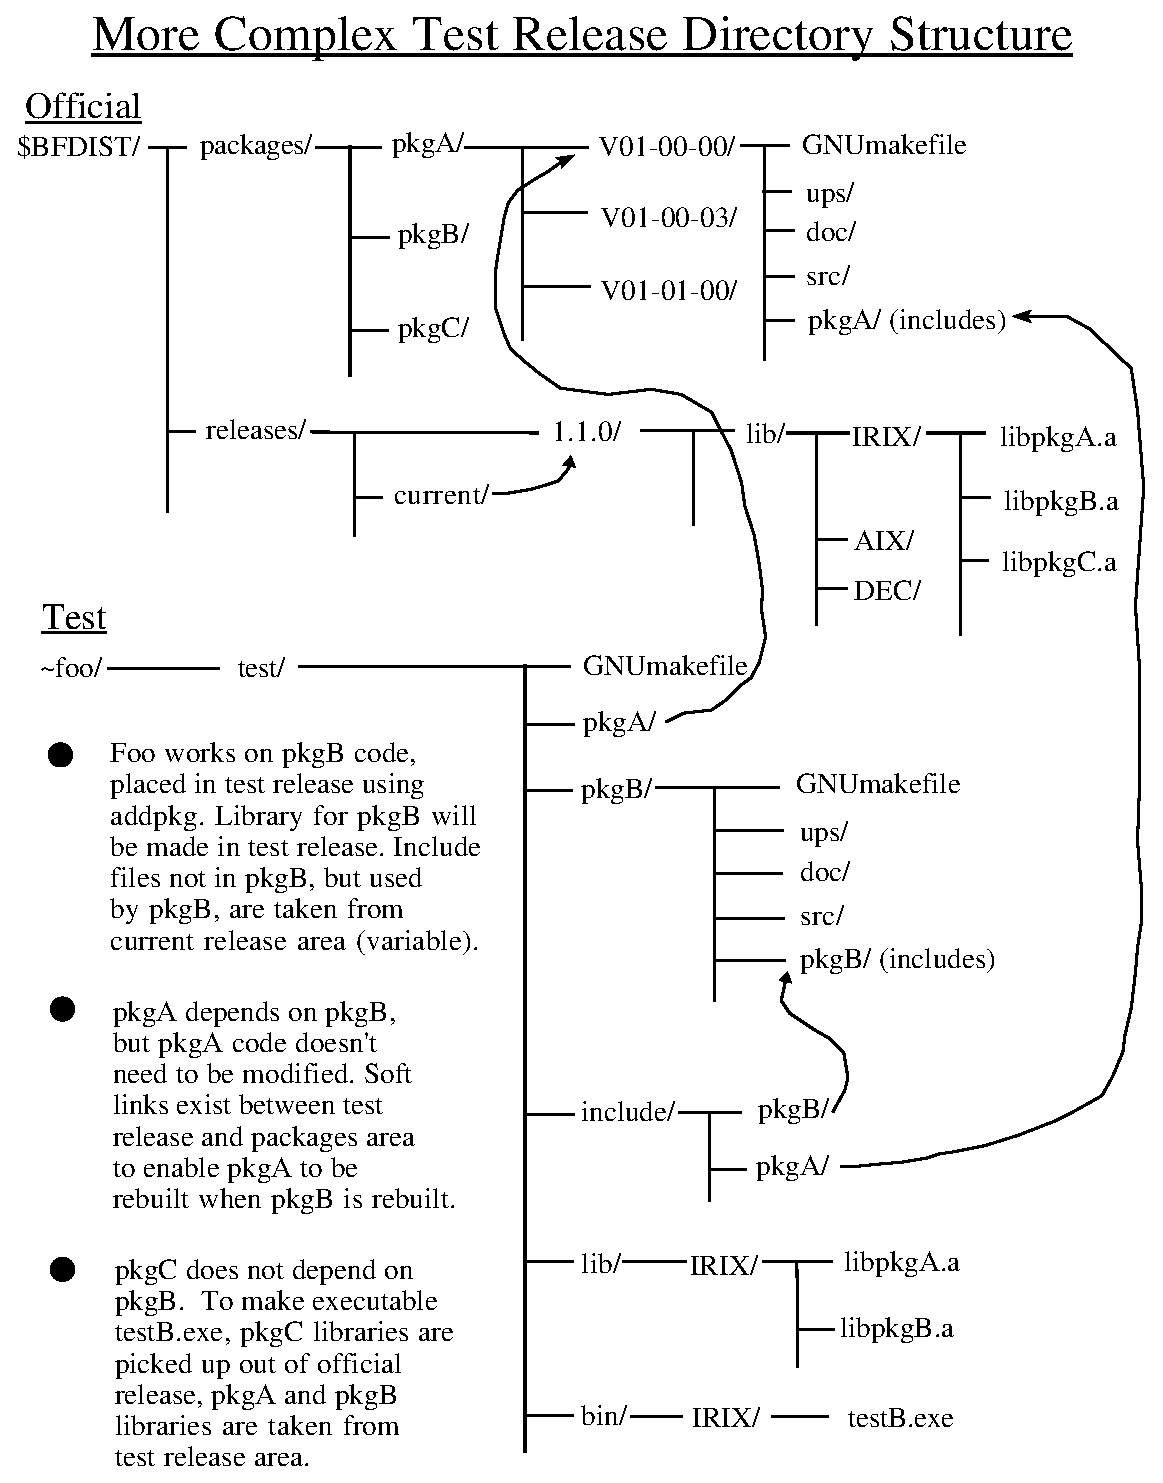
\includegraphics[width=5in]{run_2_development.eps}}
\caption[Complex Test Release Directory Structure]{ 
Diagram of a complex test release directory structure, and how it relates to the
official release directory structure.  Here the package ``pkgB'' is being
developed\index{packages!development of} , and ``pkgA'' depends on the contents of ```pkgB''. The curved lines 
\index{dependencies!complex test release} 
correspond to soft links.}
\index{soft links}
\label{fig_testrel}
\end{figure}
\clearpage 

\subsection{Distribution}
Initial distribution of the offical release structure to a remote machine will 
eventually be done via UPD once we have fully integrated it into our system.
In the meantime, we have developed simple scripts to 
initially distribute the release structure to a remote machine, 
discussed in Appendix~\ref{app_dist}.  
The release structure, those directories and soft links underneath
\index{soft links}
\$SRT\_DIST/releases in Fig.~\ref{fig_directory}, are saved in a tar file on the
server\index{client-server} machine.  
In addition, each package\index{packages!tar files}  is saved in it's own tar file. 
The location of the tarfiles on the distribution server\index{client-server} 
machines is given in ???
The
remote manager uses UPD, or currently the shell scripts described in 
Appendix~\ref{app_dist}, to copy these tar files from the distribution machine
to the remote machine and unwind them into the official 
releases\index{releases!area}  and packages\index{packages!area} 
area.  The tar file of the release specifies the flavor of the operating system and 
the version of the release. The user sets up the release using UPS as 
\index{UPS}
described in Section~\ref{sec_setup}.  The philososphy of using UPS with the
system is discussed in Appendix~\ref{app_ups}.

Once the remote machine has received an initial distribute of an official 
release, linking and development can take place. 
Distribution of the source code to a remote machine for user development is
accomplshed via SoftRelTools.  As described in section~\ref{sec_debug}, 
addpkg\index{addpkg} 
is used to checkout a complete package from CVS\index{CVS} for user development 
of that package\index{packages}. Within a test release, developers can
build and link code with their changes.  Libraries and include files from
other packages are taken from the official release. A development
release, described in section~\ref{sec_development}, can be constructed on 
any node and the code can be updated daily via CVS and rebuilt.  This is a
simple way of distributing the code to remote institutions on a daily basis,
and insuring that it works there just as well as on a central system. For
instructions on distribution of the development release at CDF, please see
section~\ref{sec_distribution_development}.

In summary, distribution of binaries and code of official 
releases\index{releases} takes place 
with UPD, after which users can link, and developers can work 
\index{linking!and distribution}
on packages  distributed to their test release by SoftRelTools.

%================================================================================
% All the appendices
%================================================================================

\clearpage
{\Huge \flushleft Appendix}
\appendix

%%%%%%%%%%%%%%%%%%%%%%%%%%%%%%%%%%%%%%%%%%%%%%%%%%%%%%%%%%%%%%%%%%%%%%%%%%%
% CVS
%%%%%%%%%%%%%%%%%%%%%%%%%%%%%%%%%%%%%%%%%%%%%%%%%%%%%%%%%%%%%%%%%%%%%%%%%%%
\section{Appendix on Version Control with CVS}
\label{app_cvs}

Concurrent Versions System (CVS)\index{CVS!introduction} is a 
freeware version control system that is widely
used by freeware developers including those in high energy physics. 
It is used by the CERN and Fermilab computing
divisions and by the following physics collaborations: ATLAS, CMS, SDSS, NuTeV,
CLEO, and BaBar.  Now it is also being used by CDF, D0 and BTeV. 
\index{BaBar}
\index{CDF}
\index{D0}
\index{BTeV}

Additional information can be found at:

\begin{itemize}
\item CVS Documentation <http://www.fnal.gov/docs/products/cvs>
\item CVSH <http://www.fnal.gov/cd/FUE/cvsh/>      
\end{itemize}

\subsection{ The CVS Repository and Basic Concepts}
\index{CVS!introduction|(}

CVS\index{CVS!repository} extends the notion of revision control from
a collection of files in a single directory, as in CMS, to a hierarchical
collection of directories each containing revision controlled files.
For example, two CVS\index{CVS!repository} repositories designed to contain the CDF offline software
\index{CDF}
\index{CDF!repositories}
are shown in Fig.~\ref{fig_repository}.      


\begin{figure}[tbh]
\begin{center}
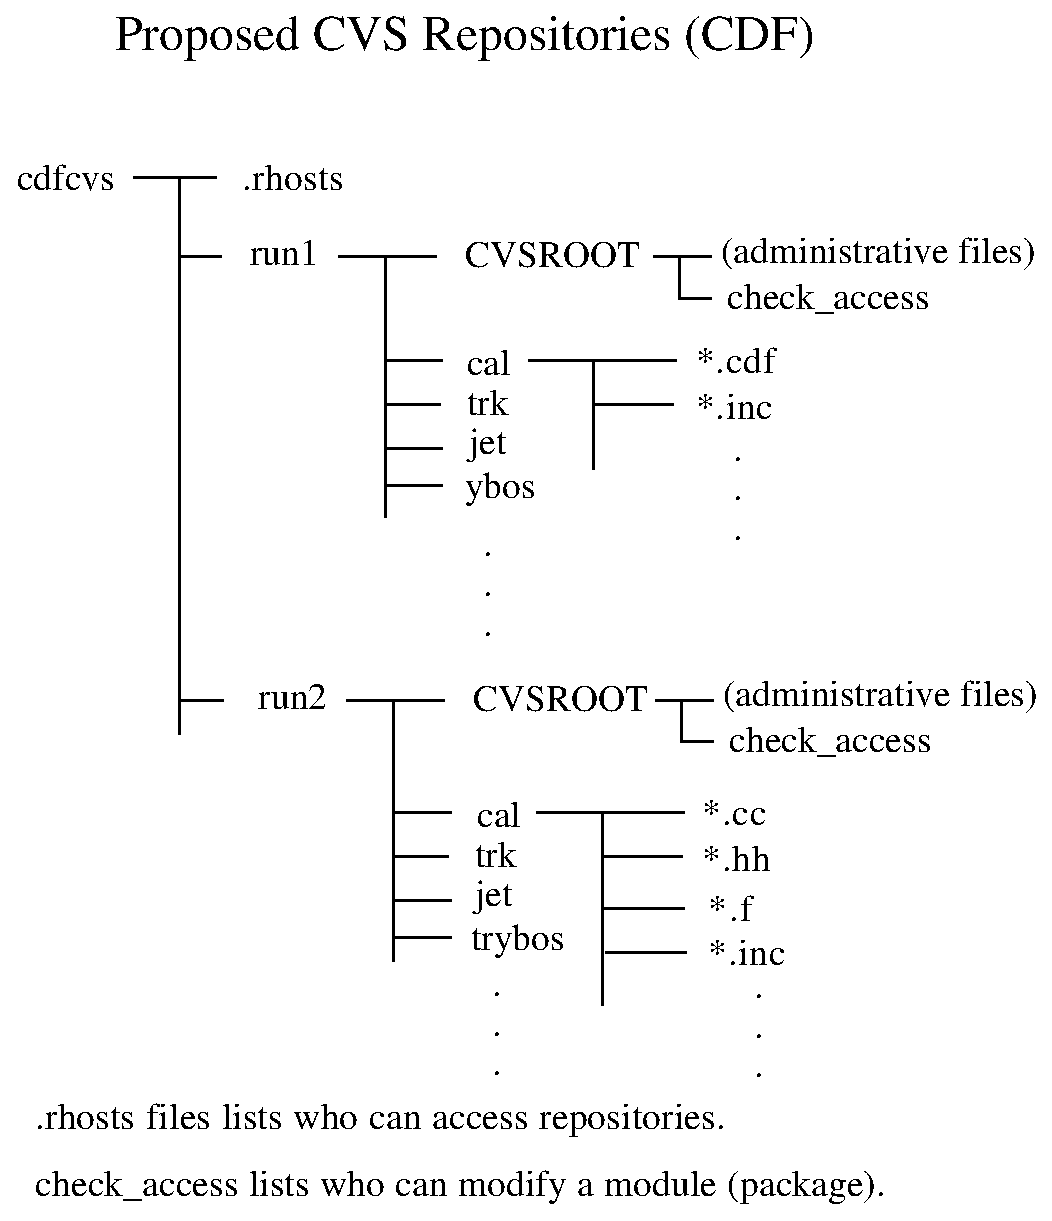
\includegraphics[width=4.0in]{two_repositories.eps}
\end{center}   

%\vspace*{-0.5in}
\caption[CVS Repositories]{
The structure of two CVS\index{CVS!repository} repositories, one for run 1 and one
for run 2.}
\label{fig_repository}
\end{figure}

Like CMS groups, CVS\index{CVS!module} collects files together into {\em modules}, and allows
operations on entire modules.  For example, the jet library would be a
module. Like a CMS class, CVS\index{CVS}
allows a collection of specific file versions to have a name, called a
{\em tag}.  CVS\index{CVS!file versions} labels each file with version
numbers, and allows branches and merging as depicted in Fig.~\ref{fig_branch}.
\begin{figure}[tbh]
\begin{center}
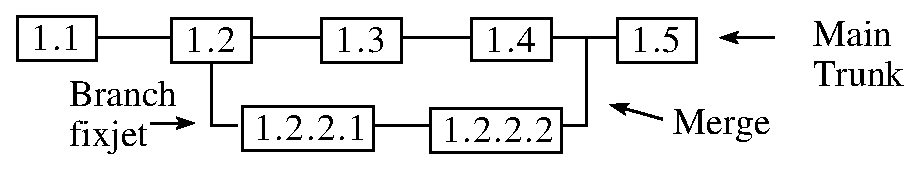
\includegraphics[width=6in]{cvs_revisions.eps}
\end{center}
\caption[Revisions, Branching and Merging]{
The versions of a particular file along the main trunk of the revision,
1.1, 1.2, 1.3, 1.4 and 1.5 are shown, along with a branch called {\ttfamily
fixjet},
that consists of modifying revision 1.2 into 1.2.2.1 and 1.2.2.2.  The
branch was merged back into the main trunk after revision 1.4 was complete,
giving revision 1.5.}
\label{fig_branch}
\end{figure}
As its name indicates, CVS\index{CVS!concurrent development} encourages concurrent revision by multiple
developers in parallel, unlike CMS which is designed for linear revision of
reserved files.  A script has been written to allow the command {\ttfamily
reserve} in CVS\index{CVS!reserve script} if desired.

\subsection{ Basic CVS Commands: A Single Revision Cycle}

As an example for the CVS\index{CVS!revision cycle} novice, the following commands perform a single
software revision cycle:
\begin{quote}
\ttfamily
cvs checkout jet/jtc90s.F\index{CVS!commands!checkout} \\
cd jet \\
cvs log jtc90s.F\index{CVS!commands!log} \\
emacs jtc90s.F \\
cvs commit -m "Changed jet energy scale!" jtc90s.F\index{CVS!commands!commit} \\
cd .. \\
cvs release -d jet \index{CVS!commands!release}\\
\end{quote}
The {\ttfamily cvs checkout}\index{CVS!commands!checkout} command creates in the users working directory a
subdirectory \texttt{jet/}, and places in \texttt{jet/} the file
\texttt{jtc90s.F}. This is like {\ttfamily CMS fetch} with an additional directory structure
created. The user goes to the \texttt{jet/} subdirectory and issues the
{\ttfamily cvs log} command\index{CVS!commands!log}, which presents her with the history of the file
\texttt{jtc90s.F}, like {\ttfamily CMS history}. The user then edits the file
(in this case using \texttt{emacs}) and places the file
back in CVS using {\ttfamily cvs commit}\index{CVS!commands!commit} and including comments, like
{\ttfamily CMS replace/keep}.  Finally the user passes back up to the working
directory and removes the entire jet/ directory tree with the command
{\ttfamily cvs release -d}\index{CVS!commands!release}, which checks to make sure there aren't any changes  
left to incorporate before deleting the files.
\index{CVS}
\index{CVS!introduction|)}

%%%%%%%%%%%%%%%%%%%%%%%%%%%%%%%%%%%%%%%%%%%%%%%%%%%%%%%%%%%%%%%%%%%%%%%%%%%
% Structure
%%%%%%%%%%%%%%%%%%%%%%%%%%%%%%%%%%%%%%%%%%%%%%%%%%%%%%%%%%%%%%%%%%%%%%%%%%%
\clearpage
\section{Appendix on the SRT Software Release Directory Structure}
\label{app_structure}

    To accommodate the storage of the various components of such a release, 
a consistent tree-structured hierarchy of directories is established. 
For expository purposes, we identify each directory with its depth (distance 
from the base) in the hierarchy. All quoted file names correspond to the 
labels in Figure~\ref{fig_directory}.

\subsection{The root directory (depth 0)}

    At the base (root) of this hierarchy is a single directory. Labelled 
``\$SRT\_DIST/'', this directory's sole purpose is to provide a starting point for 
the structure. In this root directory are entries for (the directories at the 
roots of) the two major subtrees of the structure, ``packages/''
\index{packages!area} 
 and ``releases/"\index{releases!area}. 

\subsection{The ``packages/'' directory (depth 1)}

    This directory serves as a root for the source code, documentation, 
makefiles, etc., for all versions of all packages in the product. Thus, each 
entry in ``packages/''\index{packages!area} is the starting point for a particular package. Note 
carefully that only items from the CVS\index{CVS!repository} repository are found. 

\subsubsection{Package directories ``pkgA/'', ``pkgB/'', ... (depth 2)}

    Each of these directories, direct descendents of ``packages/''
\index{packages!area} , serves as the
root of all the code, etc., associated with all versions of a single package. 
These directory names typically match the corresponding CVS\index{CVS!module} module name. Each 
such directory will have as many entries as the package has versions. 

\subsubsection{Individual version directories ``V01-00-00/", ... (depth 3)}
\label{sec_version}

    Each distinct version of a given package has its own root directory, a 
direct descendent of the package's root at depth 2 described above. The name 
of a version directory typically matches the release tag associated with the 
corresponding versions of the files in the CVS\index{CVS!tag or version} repository. 

\subsubsection{Depth 4 and beyond}
\label{sec_depth4}

    At this level, we find the source structure corresponding to (directly 
descended from the version root of) a particular version of a particular 
package. Among these entries, we might typically find: 
\begin{enumerate}
\item ``GNUmakefile'' (for the complete package)\index{packages!GNUmakefile} , 
\item  ``ups/'' (directory holding setup and unsetup files).
\index{UPS!subdirectory}
\item ``doc/'' (directory for tutorial and other documentary files), 
\item ``man/'' (directory to contain Unix-style man pages), 
\item ``src/'' (directory containing .cc and .f files), 
\item ``include/'' (directory holding .h and .inc files), 
\end{enumerate}

    Note: Figure~\ref{fig_directory} does not show all these directories, but 
they are clearly implied by the accompanying narrative. Also, 
Figure~\ref{fig_directory} labels the ``include/'' directory with the 
package name; however, this name is not a requirement of the structure but one which we 
recommend. This is because it reflects the including convention adopted in
the code: \#include pkgname/incname (see section~\ref{sec_include}).  

Recall that binary files are not intended to be located here.
However, one could conceive of additional directories here, such as ``test/'' or 
``examples/'' or ``tools/'', not necessarily part of all packages.

    The guiding principle is that, at this level, the logical structure of a 
package ought to dictate the directory structure. For reasons to become clear 
shortly, the ``include/'' directory is required, and must contain all those 
files that are visible to, and hence may be included by, any other packages or 
user software. 

The Unix-style man pages are put in the ``man/'' area of the directory 
structure. The UPS project setup file modifies the users MANPATH to include 
\index{UPS!MANPATH}
this area.

\subsection{The ``releases/'' directory (depth 1)}

    This direct descendent of the product root directory serves as a base for 
all vetted releases of the product. Each entry in this directory is the 
starting point for one such release. 

\subsubsection{Individual release directories ``1.0.0/", ... (depth 2)}

    Each of these directories, direct descendents of ``releases/", serves as the
root of all the information needed to make use of a release of the entire 
product. The name of a release directory typically matches the identification 
of a release in terms of the collection of all sources. 

    In addition, there are two standard directory names found at this level: 
``production/'' and ``current/''. These are only links to other release 
\index{soft links}
directories. They serve, however, as convenient and standardized labels so 
that users need not necessarily be cognizant of new releases: as each new 
release is installed, these directory links are intended to be broken and 
re-created as appropriate.\index{releases!soft links}

    At this level a general makefile can be created automatically to build the 
entire release tree. The makefile will simply: 
\begin{itemize}
\item invoke each of the package-specific makefiles\index{packages!GNUmakefile}  
(previously described) in turn, and 

\item install the resulting libraries and binaries into the respective 
``lib/'' and ``bin/'' flavor-specific subdirectories. 
\end{itemize}
\paragraph{\underline{Release component package directories ``pkgA/", ... (depth 3)}}

    Each of these directories corresponds to one of the 
packages\index{packages}  that make up 
the release, reflected by their parent directory, of the product. These 
directories are named for their corresponding packages. 

    However, in order to reduce unnecessary duplication of information already 
present within the ``packages/'' substructure, each of these directories is 
simply a link to the directory (at depth 3, described in 
\index{packages!soft links} 
\index{soft links}
section~\ref{sec_version} above) corresponding to the appropriate version of 
the package used to construct this release. 

\subsubsection{The ``include/'' directory (depth 3) and its descendents}
\label{sec_include}

    The intent of this directory, also a direct descendent of an individual 
release directory, is to serve as the indirect base for all .h files that 
are intended to be visible to any user of the software product. 

    This ``include/'' directory contains links, named for the individual 
\index{soft links}
\index{packages!soft links} 
packages, to the various depth 4 ``include/'' directories found under the 
``packages/'' structure (described among section~\ref{sec_depth4} above). In 
this way, code duplication is avoided, yet all include files are accessible to 
the user from one convenient source. 

The convention for including files in the source code is
 \#include pkgname/incname.
Here an 
include file, incname, is associated with a unique package, pkgname, necessary 
if two packages\index{packages!include files} have different include files with the same name.      

\subsubsection{The ``lib/'' and ``bin/'' directories (depth 3)}

    Via these directories, the remaining direct descendents of an individual 
release directory, we find a path to the software product's binaries. As is 
traditional, executables are found under ``bin/", while user-linkable libraries 
\index{linking!library locations}
are found under ``lib/". 

\subsubsection{Flavors directories ``IRIX/", ``AIX/'', ... (depth 4)}
\label{app_flavors}

\begin{sloppypar}
    These directories come into play when the software product is supported on
multiple platforms. When such is the case, ``bin/flavor/'' would serve to 
consolidate all executables for a given platform, while ``lib/flavor/'' would 
play a similar role for user-visible libraries. 
The directory is actually given a name that is a concatenation of the flavor
and version of the operating system, for example IRIX5 instead of IRIX.
This name (e.g. IRIX5) is stored in the environmental variable \$SRT\_ARCH.
\end{sloppypar}

\subsection{Usage of the directories}

    In the following sections we explain how the SRT directory structure and 
its Software Release Tools are envisioned to relate to the various client 
communities that deal with them. 

\subsubsection{A user's viewpoint}

    The UPS setup of a particular release sets the user's path, manpath, etc., 
\index{UPS!MANPATH}
\index{UPS!PATH}
in such a way that binaries are directly accessible, include files can be 
available through an environment variable pointing to the release ``include/'' 
tree, and the libraries can be used by a reference to the library tree 
environment variable via the ``-L'' compiler option. 
\index{compiler!options}

    The directory structure assumes that most users will make use of a complete
release, rather than mixing-and-matching packages across releases. If, however, 
a user would like to work with release ``A'' of a product but use version ``B'' of 
a package ``pkgC'', s/he should use the SRT ``newrel'' command to recreate the 
\index{newrel!users viewpoint}
release structure in his/her own working directory. To this command the user 
has to specify version ``B'' of package ``pkgC''. Version ``B'' of pkgC needs to 
be built in this new test release context. The user can then link his/her own 
\index{linking}
executable against this new test release. 

\begin{sloppypar}
Those users who want to write their own scripts and makefiles just need to 
know a few things. As discussed in section~\ref{sec_setup}, the UPS setup 
\index{UPS!SRT\_DIST and SRT\_CURRENT}
\index{UPS!environment}
defines the environmental variables \texttt{SRT\_DIST} and \texttt{SRT\_CURRENT}.  
The environmental variable \texttt{SRT\_ARCH} is also defined to indicate the flavor 
of operating system, as discussed in appendix~\ref{app_flavors}. In principal,
these are the only environment variables you need to use the software release 
structure. Although we strongly recommend the use of our setups and makefiles, 
the user is free to suitably define these variables to point at the right areas,
and then write their own scripts and makefiles.  The user needs to know 
that compilation with package include files\index{packages!include files}  is 
accomplished using the compilation option 
\texttt{-I\$SRT\_DIST/releases/\$SRT\_CURRENT/include}, and linking with package
\index{linking!-L option}
libraries is accomplished using the link option 
\texttt{-L\$SRT\_DIST/releases/\$SRT\_CURRENT/lib/\$SRT\_ARCH}. Users who 
prefer to do it themselves should be able to use this information to write 
their own sripts and makefiles.  However, we recommend that the provided
scripts and makefiles be used.
\end{sloppypar}

\subsubsection{A developer/contributor's viewpoint}

    In a private ``workdir'' directory, using the command ``newrel'' the developer 
\index{newrel!from developers viewpoint}
can recreate the release structure starting from a reference release. 
To modify an existing package,  the contributor can use the ``addpkg''
\index{addpkg!from developers viewpoint} command 
that checks out the module from the CVS\index{CVS!repository} repository. 
The checkout command creates the main directory structure for the package 
reflecting the module organization in CVS. Extra directories need to be 
created by the package-specific make file. The developer then 
communicates changes to the librarian, who commits them to CVS\index{CVS}.

\subsubsection{A librarian/package manager's viewpoint}

\begin{sloppypar}
    A librarian has to go through the same steps a developer goes through, but 
he has write access to the CVS\index{CVS} repository for his own 
package\index{packages!librarian}. The librarian has access to the package-specific directory in the 
\$SRT\_DIST/packages tree. This can be accomplished via a group uid, and 
trusted developers can be added or removed from this uid using the systools
commands \texttt{cmd addmember} and \texttt{cmd delmember}.
\end{sloppypar}

\subsubsection{A product/configuration manager's viewpoint}

    The product manager has write access to the entire \$SRT\_DIST tree. He can 
operate directly in the \$SRT\_DIST directories and use the ``-p'' (production) 
option of the ``newrel'' command. 
\index{newrel!managers viewpoint}

%==========================
% UPS and SRT
%==========================
\section{Appendix Using UPS with SRT}
\index{UPS}
\label{app_ups}
 
First some general comments. It is important to note that much of the 
information about which package\index{packages} 
    version works with what other package version, is contained in the release 
directory structure itself. This
    removes the requirement that this information be stored in the UPS database
\index{UPS!databases}
as dependencies. This is
\index{dependencies!UPS}
    desirable for a number of reasons. Maintaining and distributing this 
information in the form of the UPS 
    database has through the years proven to be difficult. Various recent 
additions to UPS help - cups is an
\index{UPS}
    example - but it is still true that you must be a UPS expert in order to 
\index{UPS}
effectively maintain this information. In
    a period of stable code distributions this is not a disaster; however, in a 
heavy development period it may
    become one. The other reason for minimizing UPS's knowledge of package 
\index{packages!UPS}\index{UPS}
dependencies is that it will
\index{dependencies!UPS}
    speed up and simplify the process of setting up a set of packages.
\index{packages!setup}  There 
will be fewer ambiguities about
    which versions of packages actually get setup. 

    However the concept of UPS product dependencies is still needed. There are 
\index{dependencies!UPS}
many products that we use, over
    which we have little or no control. In fact any 
package for which we do not keep
    our own CVS\index{CVS!external packages} library, would be classified in this category. Let's call 
them external packages\index{packages!external}. Examples
    would be products like cernlib or tcl/TK. These packages do not live in the 
directory structure,
    and therefore the older mechanisms for handling dependencies are still required. 
\index{UPS}
\index{dependencies!UPS}
Hopefully the coupling between
    this class of packages\index{packages!inderdependencies}  is not strong. For instance, no one would be happy if
you could only use version A of
    tcl/Tk with version B of cernlib. Also, note that references to libraries and 
binaries from this class of package are still referred to through environmental 
variables or path setting. They are not copied to the
 \verb|$SRT\_DIST/release/<version>/lib| or \verb|$SRT\_ROOT/release/<version>/bin| areas. 

\subsection{Using UPS for packages}
\index{packages!UPS} 
\index{packages!setup} 
\index{UPS!package setup}
\index{UPS}

    Packages inside the directory structure still need to be able to 
specify how environment variables,
    needed for the running of their package, must be set. For example, in the 
news product, NNTPSERVER
    must be set to the site news server machine; for tex, TEXINPUTS defines the
search list of directories to
    look for tex files. Many of the other uses of ups/setup.* files, like path 
\index{UPS}
modifying, are not needed by this type
    of package because all of the binaries live in the release structure. 
Therefore, for each
    package in the package tree, at the same level as doc, src, include and 
GNUmakefile, there is a UPS 
\index{UPS!subdirectory}
    subdirectory, which contains setup and unsetup files that are 
fragments of the
full project setup. These fragments are concatenated into the full setup 
and unsetup files in the release tree during the release build. 
Each of the fragments is a fast
equivalent of \texttt{setup <pkg>} with the appropriate version number.

\subsection{Using UPS with releases}
\index{UPS!release setup}

    In the release tree there is a UPS subdirectory at the same level as 
\index{UPS!subdirectory}
bin, lib, and include. It 
    contains a setup file that sets the path to contain the bin area of the
release and define anything else
    needed for the global release. 
From now on we refer to a global release
as a project. Thus a project is a set of experiment written products that 
get linked together into executables, and hence would form a release.  For
example online and offline could be separate projects.

The setup and unsetup file also have copied into them the 
fragments from all of the packages\index{packages!setup fragments} 
    contained in the release. These files could be built by the script that 
makes new releases\index{releases} (newrel), but currently they are build by the release 
manager by declaring the release of the project to UPS.  Marc Mengel has 
\index{UPS}
developed a utility called
\index{newrel!ups}
UPS\_COMPILE which we use to collect the fragments together into a 
\index{packages!UPS compile} 
\index{UPS!compile}
single script. The setup file
    also declares this release to the experiment UPS database so that users of 
\index{UPS!databases}
the release could say, for example, ``setup $<$project$>$ 
[$<$project-version$>$]'', as is done in section~\ref{sec_setup}.
At this time any external package dependencies could be
\index{dependencies!UPS}
defined in the UPS database.

\subsection{External Packages and UPS}
\index{packages!external} 
Not all packages used by the experiment will be included in the release 
structure. External packages, such as CERNLIB or tcl/TK or gcc, for which we 
do not usually rebuild the code, are not located in the release structure.  
They are located somewhere else which is pointed to by the normal UPS 
\index{UPS!external packages}
environmental variable.  We do not use CVS\index{CVS!external packages} to track the source code of external 
packages. There is no restriction on where the environmental variable 
\texttt{<product>\_DIR} points. If we need to rebuild external packages, we
use their own makefiles, not the SoftRelTools makefiles.

In the SoftRelTools makefiles we use the UPS \texttt{<product>\_DIR} 
\index{UPS!product variable}
environmental variables
\index{packages!external!environmental variables} 
to pickup external package libraries and include areas necessary for building.
These environmental variables may be defined through UPD dependencies, whereby
\index{dependencies!UPS}
we have declared the project to depend on a given version of an external 
package. The intent is that \texttt{<product>\_DIR} is set when we setup the
project, not via a separate ``setup $<$product$>$'' statement which might 
pickup the wrong version of the external product for the project.

%%%%%%%%%%%%%%%%%%%%%%%%%%%%%%%%%%%%%%%%%%%%%%%%%%%%%%%%%%%%%%%%%%%%%%%%%%%
% Makefiles
%%%%%%%%%%%%%%%%%%%%%%%%%%%%%%%%%%%%%%%%%%%%%%%%%%%%%%%%%%%%%%%%%%%%%%%%%%%
\section{Appendix on Makefiles in Software Release Tools}
\label{app_make}

SoftRelTools use GNU Make for building libraries and executables.
\index{gmake}
\index{gmake!GNUmakefile!user run2}
The file GNUmakefile, in the area where the gmake command
is given, tells GNU Make what to build.
%The user only needs to use
%the makefile in section~\ref{app_user_make} to link a job, and shouldn't need
%to modify it.
\index{linking}
The developer introducing a new package, or the user trying to link an
executable, needs to modify simple
makefiles described in section~\ref{app_package_make}.  Developers, code
librarians, and code managers will want to be aware of the
makefiles discussed in section~\ref{app_release_make}, but should
not need to modify them.   

\subsection{Package Makefiles}
\label{app_package_make}
\index{packages!GNUmakefile}
The following example of package makefiles, \\
\$SRT\_DIST/releases/\$SRT\_CURRENT/Framework/GNUmakefile 
and \\ \$SRT\_DIST/releases/\$SRT\_CURRENT/Framework/src/GNUmakefile, 
are used for building the libraries and executables of the Framework package.
\index{gmake}
\index{gmake!GNUmakefile!package level}
They are examples of typical package makefiles used by gmake in the examples of 
section ~\ref{sec_debug} and ~\ref{sec_newrel}. 
The first makefile only points gmake at the subdirectory src in which the
\index{gmake}
second makefile resides. The second makefile specifies the library target 
libapp.a, and includes the architecture specific makefile for the tcl package, 
on which the framework package depends.  Both makefiles include standard.mk 
which defines the compilation and dependency generation in detail.
\index{BaBar}
\begin{footnotesize}
\begin{verbatim}
$SRT\_DIST/releases/$SRT\SRT\__CURRENT/Framework/GNUmakefile 
# GNUmakefile for the BaBar Framework package
#
# uses SoftRelTools/standard.mk
#
#    Bob Jacobsen, Jan 96
#
#############################################################
# file lists (standard names, local contents)

# include file products
INC =

# library product
LIB =

#library contents
LIBFFILES  =
LIBCFILES  =
LIBCCFILES =

# subdirectories
SUBDIRS = src

# binary products
BINS =

############################################################
include SoftRelTools/standard.mk
\end{verbatim}
\end{footnotesize}
\vspace*{1in}
\begin{footnotesize}
\begin{verbatim}
$SRT_DIST/releases/current/Framework/src/GNUmakefile 
# new Makefile for Framework - the old one is unchanged.
#
# uses SoftRelTools/standard.mk
#
#############################################################
# file lists (standard names, local contents)

# include file products
INC =

# library product
LIB = libapp.a

#library contents
LIBCFILES  =
LIBCCFILES := $(shell ls *.cc)


# binary products
BINS =

# APPMain.o is required for Solaris link
all:
lib: $(libdir)/APPMain.o
$(libdir)/APPMain.o: $(libdir)/$(LIB)
        cd $(libdir); ar x $(LIB) APPMain.o
include SoftRelTools/arch_spec_Tcl.mk

############################################################
include SoftRelTools/standard.mk
\end{verbatim}
\end{footnotesize}


\subsection{Release, Standard, and Architecture Specific Makefiles}
\label{app_release_make}
At the top of every release is a GNUmakefile as shown in 
Fig.~\ref{fig_directory},~\ref{fig_dev_simple}, and ~\ref{fig_testrel}. The 
release makefile recognizes the experiment by 
means of the .experiment file, which contains names like CDF or D0. The release
\index{CDF}
\index{CDF!.experiment file}
\index{D0}
\index{D0!.experiment file}
\index{.experiment file}
makefile specifies what areas will be searched for include files when
compiling, and what areas will be searched for libraries when linking.
\index{linking}
Most important, for the library and executable targets, this file effectively 
loops over the individual package makefiles and runs make for them.
The release makefile is the heart of the building system.

The user makefiles and package makefiles described in the last section
includes the makefile standard.mk.  This makefile contains standard target 
definitions and rules for compilation and linking.  Similarly, standard.mk
\index{linking}
includes the file arch\_spec.mk, which contains the architecture specific
rules for each machine and operating system.
\clearpage



\clearpage
\addcontentsline{toc}{section}{References}
\begin{thebibliography}{99}

\bibitem{ref_sdss} CVS at SDSS is described on the Code Management WWW pages
at http://www-cdf.fnal.gov/offline/code\_management/sdss.html.
\index{CVS!SDSS-CVS}

\bibitem{ref_babar1} Bob Jacobsen, ``The BaBar Software Release Structure'',
\index{BaBar}
March 5, 1995, on the WWW at
http://www.slac.stanford.edu/BFROOT/dist/releases/current/SoftRelTools/ 
SoftRelToolIntro.ps.

\bibitem{ref_babar2} Bob Jacobsen, ``Using the BaBar Software Release 
Structure'', October 28, 1995, 
http://www.slac.stanford.edu/BFROOT/doc/Computing/Reconstruction/Notes/
SoftRelToolUser.ps.

\bibitem{ref_tuura} Lassi A. Tuura, ``Helper programs for Moose Directory
Structure'', http://wwwcn1.cern.ch/l/lat/www/notes/soft/dist/scripts.html.

\bibitem{ref_commentary} Walter Brown, Flavia Donno-Raffaelli and Elizabeth
Sexton-Kennedy, ``On the Software Release Directory Structure'' on the Code
Management WWW pages at 
at http://www-cdf.fnal.gov/offline/code\_management/srt.html.

\bibitem{ref_REBUILD} Flavia Donno-Raffaelli, ``REBUILD Users Guide and
Reference Manual'', CDF Note 1611, August 15, 1994.  Available on the WWW at
http://www-cdf.fnal.gov/offline/code\_management/rebuild.mem.

\bibitem{ref_cmgt_c++} See discussion of C++ implications on Code Management
\index{C++}
pages on the WWW at 
http://www-cdf.fnal.gov/offline/code\_management/c++.html.

\bibitem{ref_cvs} Basic information on cvs is available from the man pages 
and at http://fnnews.fnal.gov/cd/UNIX/cvs/cvs.html. The complete manual can
be obtained from http://www.loria.fr/$\sim$molli/cgi-bin/wilma.cgi/doc.
\index{CVS!references}.  A hardcopy of this manual is available in the CDF 
trailers office 149-E.

\bibitem{ref_cyclic} Information on Cyclic Software is available at 
http://www.cyclic.com/.

\bibitem{ref_uaf} ``UNIX at Fermilab'', Computing Division Document GU0001, 
available on the WWW at
http://www.fnal.gov/docs/UNIX/unix\_at\_fermilab/welcome.html

\bibitem{ref_alan} Alan Jonckheere, ``Configuration Management: A Turnkey 
System'', on the WWW at 
http://d0www.fnal.gov/\texttt{~}jonckheere/cmgt/turnkey.html

\bibitem{ref_dcd} Mathew Wicks, ``Fermi UNIX Environment DCD Products User
Guide'', DCD0003, DCD User Guide 3.4, January 19, 1993.

\bibitem{ref_cmgt_draft} ``Run 2 Code Management Report'', by Configuration 
Management Working Group on July 12, 1996, available on the WWW at 
http://fnpspa.fnal.gov/Run2/document.html.
\end{thebibliography}

%Index Cross References
\index{dependency files|see {.d files}} 
\index{deleting|see {removing}}
\index{get ! package|see {addpkg}}
\index{get ! test release|see {newrel}}
\index{information!about release|see {statusrel}}
\index{information!about repository|see {lscvs}}
\index{link ! symbolic|see {soft links}}
\index{link ! soft|see {soft links}}
\index{packages!installing production|see {newver}}
\index{packages!removing production|see {rmver}}
\index{packages!creating release|see {newrel}}
\index{packages!interdependencies|see {depend}}
\index{packages!soft links|see {lnkpkg}}
\index{packages!getting|see {addpkg}}
\index{packages!removing release|see {rmrel}}
\index{release!listing contents|see {statusrel}}
\index{release!creating|see {newrel}}
\index{release!removing see {rmrel}}
\index{removing!releases|see {rmrel}}
\index{removing!packages|see {rmver}}
\index{new ! production package|see {newver}}
\index{soft links!creating|see {lnkpkg}}
\index{compile!UPS |see {UPS}}
\index{UPS!dependencies|see {dependencies|UPS}}
\index{server|see {client-server}}
\index{linking!executable filename|see {EXENAME}}
\index{linking!.opt filename|see {OPTFILE}}
\index{make|see {gmake}}
\index{preprocessor|see {CPP}}
\index{version!control|see {CVS}}

\clearpage
\addcontentsline{toc}{section}{Index}
\documentclass[12pt]{article}
\usepackage{graphicx}
\topmargin -1in
\textwidth 6.5in
\textheight 9.5 in
\oddsidemargin 0.0in
\evensidemargin 0.0in
\baselineskip 14pt
\makeindex
\def\see#1#2{{\em see\/} #1}
\begin{document}
\begin{flushright}
\vspace*{0.5in}
CDF Note: CDF/DOC/COMP\_UPG/PUBLIC/3891 \\
\index{CDF}
D0 Note: 3118f \\
\index{D0}
Computing Division Note: GU0013 \\
\end{flushright}
\vspace{0.5in}
\begin{center}
{\LARGE SoftRelTools User's Guide}\\
\vspace{.5in}
{\large Version 2.0}\\
{\large \today }\\
\vspace{.5in}
{\large Last edited by Margaret Votava}\\
{\large \em Fermilab Computing Division}\\
\vspace{.5in}
{\large for:\\
Dave Adams, Jim Amundson, Jim Bellinger, Walter Brown, Glenn Cooper, 
Flavia Donno-Raffaelli, Lynn Garren, 
Herb Greenlee, Robert Harris, Alan Jonckheere, Robert Kennedy, Arthur Kreymer, 
Qizhong Li, Don Petravick, Ruth Pordes, Lars Rasmussen, 
Elizabeth Sexton-Kennedy, Scott Snyder and Gordon Watts.}
\vspace{.5in}
\end{center}
\begin{abstract}
This is the user's guide for the Fermilab version of Software Release Tools, 
a UNIX based software management system for large, collaborative projects
that is used by several experiments at Fermilab.
The system provides software version control with CVS\index{CVS} 
configured in a client-server\index{client-server} mode.
For management and 
building we have adopted the directory structure and SoftRelTools originally 
developed by the BaBar collaboration. 
The system handles the 
version control, management, building, and distribution of code written in 
Fortran, C and C++. A distinguishing feature of the system is its
\index{C++}
ability to allow rapid asynchronous development of 
package versions, 
which can be easily integrated into complete consistent
releases\index{releases} of the entire offline software.  This 
has reduced the time it takes for new and modified code to be made available to 
users. 
\end{abstract}

\clearpage
\tableofcontents
\listoffigures
\listoftables

\clearpage
\section{Introduction}

This document is the User's Guide for SoftRelTools (SRT). It is meant
to give an overview of the SRT environment and commands
from a code developers point
of view. Code librarians should refer to the SRT Reference Guide for
more detailed explanation of the SRT configuration parameters and commands. 

SRT is very flexible in the style in which it allows developers to operate. 
This flexibility presents a difficulty in writing a general purpose "how to"
User's Guide because each librarian has imposed a cycle that is most 
appropriate for that particular release and a naming convention that
best suits the cycle. Users should refer to the specific instructions 
for a given release for the naming conventions and the development cycle. 

Release specific instructions can be found at:
\begin{itemize}
\item CDF Run 2
\item D0 Run 2
\item SDSS
\item ZOOM
\item BTeV http://www-btev.fnal.gov/internal\_documents/code/code\_management.html
\item Minos 
\end{itemize}

\subsection{What is SRT}

SoftRelTools (SRT) is a toolset for managing large software projects, aka releases,
that consists of smaller units, aka packages, that are developed in parallel
by a diverse programming community. It allows individual developers to 
work on their package independently of the ongoing work in other packages,
and to update the whole project when they are satisfied with their 
modifications. In this way, the developer is responsible for the management
of his individual package, while the release librarian is responsible for 
management of the all the packages as a whole.


\subsection{How to use this document}
This document has been written in the style of a book, or pedagogical users
manual, with discussion and illustrations.  People seeking a general 
overview of the system may want to read the normal sections, omitting the 
appendices.  New users or developers who want to do something with the system 
quickly, and don't want to read much, are advised to follow the examples in 
section~\ref{sec_examples} and Appendix~\ref{app_build}. Those seeking a 
reference manual for answering arbitrary questions about the system will find
it quickest to use the index at the back of the document.  

\subsection{Other light reading}

For sleepless nights:
\begin{itemize}
\item SRT Reference Guide
\item CVS User's Guide http://www.fnal.gov/docs/products/cvs/
\item gmake User's Guide http://www.fnal.gov/docs/products/gtools/make.1.html
\item Barbar SRT document
\item CVSH http://www.fnal.gov/cd/FUE/cvsh/ 
\end{itemize}

\section{Software Release Structure}
The software release structure provides a flexible and easy to use
framework for both releasing and developing code.  Code is typically grouped
into {\em packages}\index{packages!definition}; however, it is essential to have a {\em release} of all 
code in 
all packages. The structure must support simultaneously both
releases\index{releases} of stable versions of the 
packages\index{packages}, and asynchronous development of 
the individual packages themselves.  This is in contrast to a structure which
is oriented solely along the lines of a release, where package versions
are only stamped with the release number. The BaBar software release
\index{BaBar}
structure~\cite{ref_babar1,ref_babar2}, which supports both
asynchronous development of packages\index{packages!asynchronous development} 
and grouping packages\index{packages} into 
releases\index{releases!definition},
is shown in Fig.~\ref{fig_directory}. A commentary on this structure with 
a detailed verbal description of Fig.~\ref{fig_directory} is given in 
Appendix~\ref{app_commentary}.

The environmental variable {\ttfamily \$SRT\_DIST} is used as a root to add flexibility.  
Below it are found separate subtrees for packages\index{packages} and releases\index{releases}. 
Within the
package subtree, each package can contain one or more different {\em versions}.
This allows the package librarians to develop packages 
asynchronously\index{packages!asynchronous development},
and assign the package a version number when the package is ready for use
by others.  Within the release subtree, there is a subdirectory for each
existing release.  A release directory consists of soft links to a set of 
\index{soft links}
consistent package versions, plus the libraries and binaries created from
the release for various machine architectures.  Again, the release manager
can use this to create releases\index{releases} as required.  Links within the release
\index{soft links}
directory can be used to provide default names for particular releases, for
example ``current'' for the release recommended for general use at the present
time.

Notice that the soft links between releases\index{releases!soft links} and 
packages\index{packages!soft links} are
\index{soft links}
to the source code only; the libraries and binaries are native to the release.
This is necessary because in C++ a change to a header file used by package A can
\index{C++}
affect the result in package B which uses package A, even if package B does 
not use the part of the header file that is changed or added.  Unlike common
blocks in Fortran, where you can add to the end of a common block which is
used by many packages\index{packages} and you do not need to recompile all the code, in C++
\index{compile}
\index{C++}
if you modify a header file you have to recompile all the code that depends on 
\index{dependencies!and C++} 
that header file. The only way to insure consistent results when
changing a header file is to rebuild both libraries.  

\begin{figure}[tbh]
%\centerline{\epsfig{figure=run_2_directory.eps,width=4.5in}}
\begin{center}
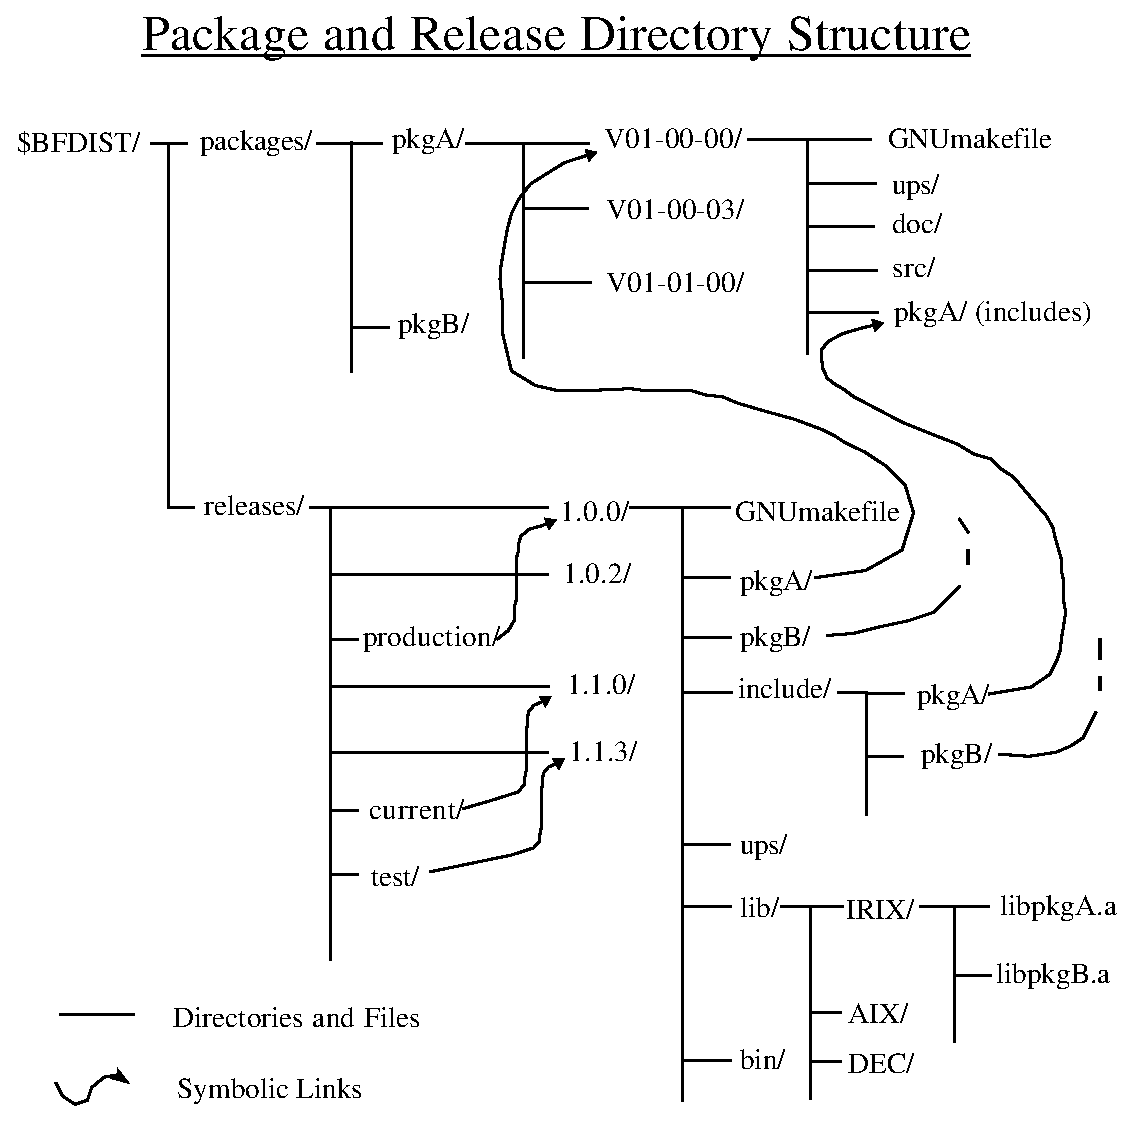
\includegraphics[width=4.5in]{run_2_directory.eps}
\end{center}
\caption[Official Release Directory Structure]{ 
Diagram of the directory structure.  This example includes two
packages: 
``pkgA'' and ``pkgB''\index{packages!definition}\index{packages!figure}. 
The curved lines correspond to soft links\index{soft links} between 
releases\index{releases!definition}\index{releases!figure} and packages.}
\label{fig_directory}
\end{figure}

\subsection{Package and Release Versions and Labels}
\index{version!of package}
\index{version!numbering convention}
The package and release numbering system is designed to allow multiple versions
of packages\index{packages!numbering} and many releases\index{releases!numbering} of code to be available to the collaboration.

The convention for package version numbers is Vxx-yy-zz where
xx is the major version field, yy the minor field, and zz is a bug fix
field incremented for small changes. This version number is also the 
CVS\index{CVS!tag or version} tag of 
that version. The first version is then V00-00-00.
The code manager will install this tag on the initial version of
the code in the repository, and either librarians or the code manager can tag 
subsequent versions using the CVS\index{CVS!commands!rtag} command rtag.

The convention for releases\index{releases!numbering} is x.y.z, where x is the 
major release number\index{releases!major},
y the minor release\index{releases!major}, and z is a bug fix 
number\index{releases!bug-fix}. Thus 1.0.0 would be a major
release that is rigorously tested,  1.1.0 would be a minor release based on 
1.0.0 and would require less testing, and 1.1.3 would be a bug fix or fast 
release based on 1.1.0 and might have almost no testing.  The ``production''
release would generally be a symbolic link to a major release, like 1.0.0.
\index{soft links}
The ``current'' release could be a minor release, like 1.1.0. The ``test'' release 
could be bug fix release, such as 1.1.3.  There could be many major, minor,
and bug fix releases\index{releases!bug-fix}, and only a few of them might have symbolic links pointing
\index{soft links}
to them with names like ``production'', ``current'', ``test'',
``fast-tracking'', etc.
This labelling system allows many different releases, and the level of
validation\index{releases!validation} is apparent from the number.

\subsection{Development Releases}
\label{sec_development}

\index{development} 
In addition to frozen releases with specific versions, SRT structure
also supports a more dynamic development environment. A development release is 
not required, but it is a very useful option for integration, bug detection,
and access to the most recent available code. Most often, 
developers are making changes on different packages in parallel. At
various stages during this development, they will want to share there
work with others. Making a frozen release for each of these stages
would consume a lot of disk space in addition to being a code librarian's
nightmare. 

In Fig.~\ref{fig_development_release} we show the structure of a development
release, which is nearly identical to a frozen release.  The difference is that
the soft links all point to the ``development'' version of the package in the
packages area.  The development version of the package was checked out of
CVS when the package was first added to development, and every day the 
development version is updated via a {\ttfamily cvs update} command. The 
{\ttfamily cvs update} command is a convenient way of distributing 
development, sending only the code that has changed from the repository to the 
development release.  Since we use client-server cvs, all nodes in the system 
are equal, and the process of getting development on a central system is no 
different than the process of getting development anywhere.  Note that no
development actually takes place in the development package area. Developers
are required to develop code in their test releases (see next section) and check
that code back in to the repository, so that the code can propogate to all
development nodes everywhere. 

\begin{figure}[tbh]
%\hspace*{0.1in}
%\epsfysize=6in
%\epsffile[36 100 581 674]{development_release.ps}
%\centerline{\epsfig{figure=development_release.eps,width=4.5in}}
\centerline{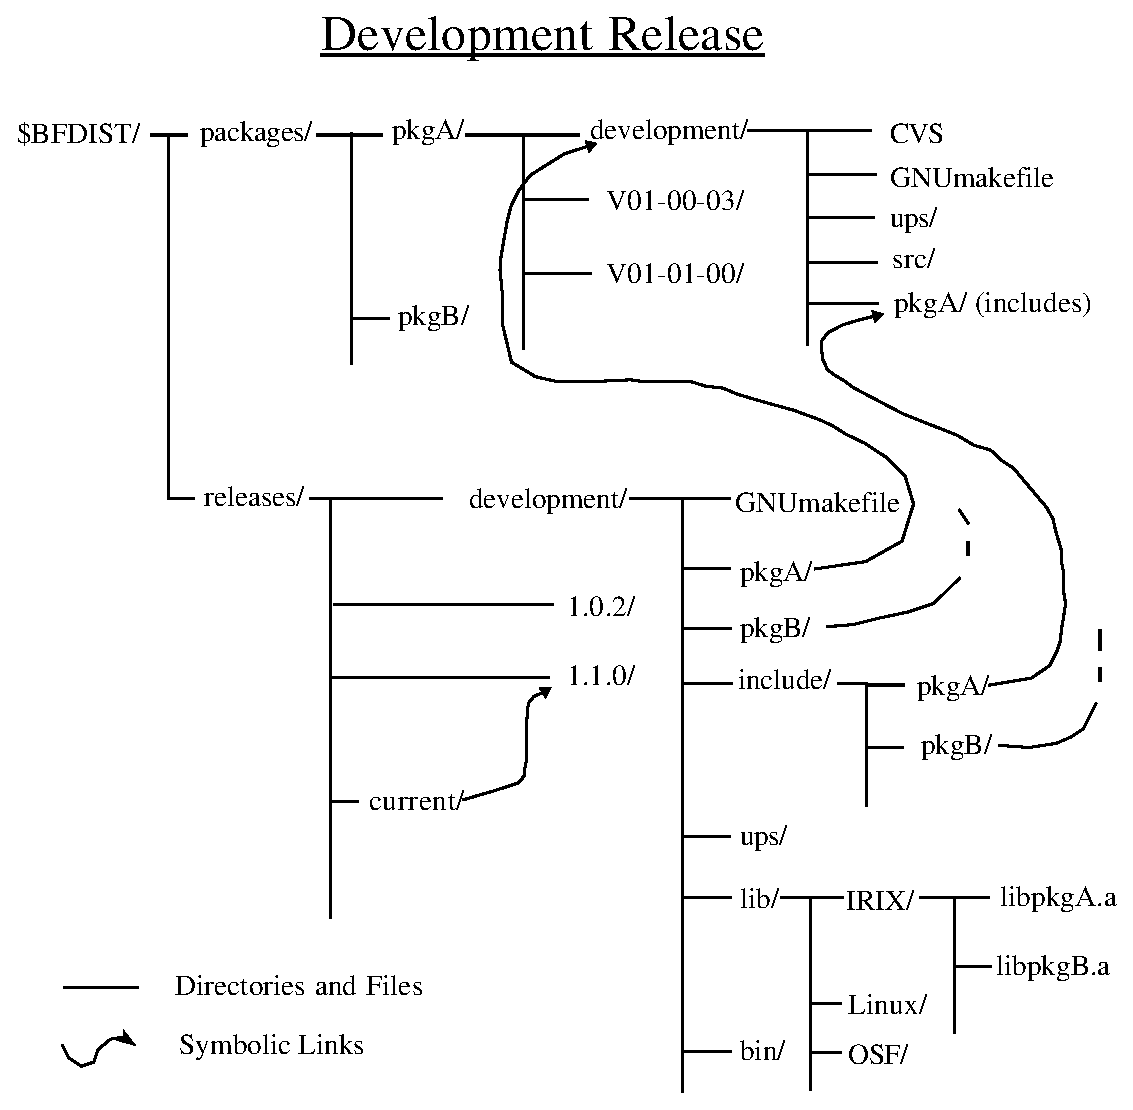
\includegraphics[width=4.5in]{development_release.eps}}
\vspace*{-0.5in}
\caption[Development Release Directory Structure]{ 
Same as Fig.~\ref{fig_directory} except the release called development
contains soft links to the development version of each package, which is 
checked out from CVS and updated from the main repository. There is nothing
hardwired about the tag "development", and each environment may have a 
different term. Please check the specific instructions from your code 
librarian.}
\label{fig_development_release}
\end{figure}

\index{development!update} 
At some interval on each development node 
{\ttfamily cvs update} is done for each package in the release, and 
then the release is rebuilt with the command {\ttfamily gmake}. At
CDF this happens every morning. Developers
can then use the development release to link against.  

A facility exists in 
SoftRelTools to scan the log files that result from the build,
find compilation and linking errors, and send error reports to the designated
developers and package librarians.  
\index{development!error reporting} 
This provides developers with immediate
feedback, and errors are caught and fixed quickly.  
This SoftRelTools error\_reporter facility
also can create error status tables, like the on in Fig.~\ref{fig_status_table}.
Ask your code librarian for links to the location of these log files. 

Although naive users may want to use a frozen release, for stability, 
in a rapidly developing software environment, developers need to use 
the development release to insure that their additions really work with
the most recent software.  

\begin{figure}[tbh]
%\centerline{\epsfig{figure=status_table.eps,width=4.5in}}
\centerline{\includegraphics[width=4.5in]{status_table.eps}}
\vspace*{-4.7in}
\caption[Status Table for Development Release]{ 
Example summary of errors detected during one night's build of the 
Run 2 development 
software at CDF. The lib stage is the compilation stage of the package,and 
the bin stage is the compilation and linking of executables for that package.
A text entry in the table indicates there was an error for the package 
indicated. Here for example there was an error linking an executable in the
TrackingMods package under Linux using the KAI compiler, and no errors 
anywhere else. This summary was generated on Wed Jul 22 08:00:19 1998 by the
error\_reporter facility in SoftRelTools.}
\label{fig_status_table}
\end{figure}

\subsection{Using the Software Release Structure}
\label{sec_examples}

This section will describe the overall procedures needed to develop
in an SRT environment.  In short, a user wants to develop a certain
package. He needs to define a context, or base release, in which this 
package will be compiled and linked. He must define a "test" release
in some working area, then copy the package to be modified
into this working area, and finally set symbolic links for header files
and libraries to the other packages in the base release - see Figure ???. 

The user is afforded many options to globally describe his development 
environment. One of which is a "super" test release. 
Look at figure ???. The default SRT behavior is to define
the path for header files to include both directories in the test 
release as well as the base release. If a user deleted a header file from 
package B in the test release, the make files would still find it in the
base release. This can lead to some confusion. SRT supports the concept
of a "super" test release which will only look for include files in the
test release. It does this by creating a directory called "super" in the
test release and putting links to each pacagke's header files therein. 


The SoftRelTools commands themselves are defined in more
detail in Section ~\ref{sec_commands}. 
Once again, you should
refer to your code librarian's instructions for the naming conventions and
practices unique to your specific configuration. Section~\ref{sec_setup}
describes how to setup SoftRelTools, necessary before any SRT 
commands can be executed.
Section~\ref{sec_debug}                                
describes constructing a test release using {\ttfamily newrel} \index{newrel} 
for development
of a package obtained using {\ttfamily addpkg}.\index{addpkg}  
This is also how a user links a job.
Section~\ref{sec_newver} describes making the new package version official 
using {\ttfamily newver}\index{newver}. Section~\ref{sec_newrel} describes making a new
production release, including the new package version, using {\ttfamily newrel}.

\subsubsection{Setup}
\label{sec_setup}
Because it is flexible and each distribution has opted for different
features, setting up the environment is the most confusing part of using 
SRT. The user needs to work out of a test release. If he doesn't already have
one, he needs to create one with the SRT "newrel" command. This only needs
to be done once, and the user can work from the this area indefinitely. 
Additionally, the user needs to run srt\_setup in each shell that his wishes
to develop in, ie, each time he logs in or creates an xterm. There is a bit
of a chicken and egg problem here in that some srt\_setup switches require that
a test release already have been created (e.g., -A), but you can't create the 
test
release until srt\_setup has been run. The solution is to execute srt\_setup
twice. 

Note that the user can have more than one test release and switch between 
them, but this is not recommended for the novice SRT user. An additional note
is that if you have if you have done an srt\_setup -A and switch test 
releases, you need to run srt\_setup again. 

SRT is very loosely coupled with UPS. It has no requirements on UPS itself,
but is modelled after it. Certain environment variables must be defined, 
e.g., ??? SRT\_DIST in a global file and then srt\_setup run. Code librarians
have wrapped this distribution specific scripts. 
Again, check with your code librarian for your specific instructons. 

For example, below are
the Run 2 setup commands at CDF and D0 (for a more complete list see ???
\index{CDF}
\index{CDF!setup}
\index{D0}
\index{D0!setup}
):
\begin{enumerate}
\item {\ttfamily source /d0library/d0local.login }\\
{\ttfamily setup D0RunII [<base-release>]}\\
\index{D0}
This will setup the D0 Run II software.  
\item {\ttfamily source $\sim$cdfsoft/cdf2.cshrc}\\
{\ttfamily setup cdfsoft2 [<base-release>]}\\
This will setup the CDF Run II software. \\
\end{enumerate}

where the files \texttt{d0local.login} and 
\texttt{cdf2.cshrc} define the UPS databases for D0 and CDF in Run II:
\index{UPS!databases}
\index{CDF}
\index{CDF!UPS databases}
\index{D0}
\index{D0!UPS databases}
the appropriate file can either be sourced 
interactively or in the users \texttt{.login} file.  


How does it know SRT\_DIST???
The setup commands define the  SoftRelTools enviromental variables 
\texttt{SRT\_DIST}, \texttt{SRT\_BASE\_RELEASE}, and \texttt{SRT\_ARCH}. 
\texttt{SRT\_DIST} is the
main directory, \texttt{SRT\_BASE\_RELEASE} is the release 
identifying name
or number in the \texttt{\$SRT\_DIST/releases} directory, and \texttt{SRT\_ARCH} 
specifies the UNIX operating system type and version number.
\texttt{<base-release>} is an optional
argument specifying the release, and if absent will default to the current
release. Note that \texttt{SRT\_BASE\_RELEASE} is not
a pathname.  For example, the \texttt{SRT\_BASE\_RELEASE} release would be found at
\texttt{\$SRT\_DIST/releases/\$SRT\_BASE\_RELEASE}, so \texttt{SRT\_BASE\_RELEASE} could be a name 
like ``current'' or
a number like ``1.0.4''.  In addition, if using in a UPS environment, it 
defines a convenient 
\index{UPS!project variable}
environmental variable (\texttt{<project>\_DIR}, which is 
\texttt{CDFSOFT2\_DIR}, \texttt{D0RUNII\_DIR}, etc.) which 
points at the area \texttt{\$SRT\_DIST/releases/\$SRT\_BASE\_RELEASE}. 
Libraries and include 
files from packages\index{packages} will be taken from the \texttt{<project>\_DIR} area, 
when linking and compiling, unless another area is specified 
by a test release (see section~\ref{sec_debug}). 

\subsubsection{Creating a test release}
\label{sec_testrel}

As previously stated, the user needs to create a working area in which
to make his changes. This is called a test release and is created with
the SRT command newrel.  This command need only be executed once per
test release directory. 

Once the test release is created, the user needs to populate it 
with the particular packages he wishes to modify via the lnkpkg command. 
Let's say that header files in a second package depend on the package the
user wants to modify. The user will want to build the libraries in 
the second package, but not modify the code. He can add the second package
to the test release via the lnkpkg command. 

\begin{itemize}
\item {\ttfamily cd <wherever>}\\
      For example, in Figs.~\ref{fig_dev_simple} and ~\ref{fig_testrel},
the user typed {\ttfamily \verb|cd ~foo|}.
\item {\ttfamily newrel -t <base-release> <new-release>} \\
\index{newrel!general use by developers}
     The "-t" switch is required and tells newrel that this is a developer's
working area and NOT a new official release to be created in \$SRT\_DIST. 
<base-release> is the official release to work off from. In many cases,
this is development. <new-release> is the arbitrary string that you
define to be your working directory. 
For example, in Figs.~\ref{fig_dev_simple} and ~\ref{fig_testrel},
the developer typed {\ttfamily newrel -t current test}.

This created the {\ttfamily test} directory and populated it with the main 
GNUmakefile and empty sub-directories include, lib, and bin, etc.  
It did not
create the {\ttfamily pkgA} or {\ttfamily pkgB} directories.
The release number 
\texttt{<base-release>} is written to a file \texttt{.current}, used by 
\texttt{GNUmakefile} to determine which production release to use.
\item {\ttfamily cd <new-release>} \\
For example, in Figs.~\ref{fig_dev_simple} and ~\ref{fig_testrel},
the user typed {\ttfamily cd test}.
\item {\ttfamily srt\_super\_init } \\
	This is an optional command that should be executed if the user
wants super test functionality. 


\item {\ttfamily addpkg [-h] <package> [<tag>]}\\
\index{addpkg!general use by developers}
This checks out the package from CVS\index{CVS!commands!checkout} to create the package sub-directory
and its contents. 
For example, in Figs.~\ref{fig_dev_simple} and ~\ref{fig_testrel},
the user typed {\ttfamily addpkg <pkgB>}.
\index{addpkg}
Note that this will check out of CVS\index{CVS!tag or version} the 
version of \texttt{<package>} that was used
to make the \texttt{<base-release>}.  This may not be the head version of the 
package,
however, it is a version that is garanteed to work with 
\texttt{<base-release>}.  If
the developer instead wants to modify the head version in CVS\index{CVS!tag or version} (the latest 
version along the main trunk), then the -h option must be used with addpkg.
\index{addpkg!-h option}
The developer should be aware that the head version is not guaranteed to 
work with the \texttt{<base-release>}.

If \texttt{<tag>} is present, {\ttfamily addpkg} does a 
{\ttfamily cvs checkout -r<tag> package}.  
\index{CVS!commands!checkout}
\index{CVS!tag or version}
\index{addpkg!tag or version argument} In
Figs.~\ref{fig_dev_simple} and ~\ref{fig_testrel}, the user typed 
{\ttfamily addpkg pkgB} \index{addpkg}
to create the sub-directory {\ttfamily pkgB} and fill
{\ttfamily pkgB} with sub-directories and code from CVS. {\ttfamily addpkg} 
\index{CVS}\index{addpkg!creates soft links}
also creates a soft link between the test release include area and the newly 
created package include area.  For example, in 
Figs.~\ref{fig_dev_simple} and ~\ref{fig_testrel}, {\ttfamily addpkg}
\index{addpkg!soft links}
created a symbolic link \verb|~foo/test/include/pkgB/| which points to
\verb|~foo/test/pkgB/include/|. 

In Fig.~\ref{fig_testrel} there is a package, {\ttfamily pkgA}, which 
depends on include files in {\ttfamily pkgB} that user Foo will modify.  
However, Foo does not need to modify any of the code in {\ttfamily pkgA}, 
Foo only wants to modify {\ttfamily pkgB}.  To allow Foo to rebuild the 
libraries for {\ttfamily pkgA} without checking out the code for {\ttfamily
pkgA}, we have created symbolic links between the test release and the
official packages\index{packages!soft links} area.  The symbolic link \verb|~foo/test/pkgA/| points to 
\$SRT\_DIST/packages/pkgA/1.1/, and the symbolic link 
\verb|~foo/test/include/pkgA/| points to \$SRT\_DIST/packages/pkgA/1.1/include/.  
The SoftRelTools script {\ttfamily lnkpkg} 
\index{lnkpkg}
creates these 
links between the test release area and the desired version of the package
(see Appendix~\ref{app_lnkpkg}). You can figure out which packages you need
to link to by running the SoftRelTools script \texttt{depend} 
\index{packages!interdependencies}
\index{depend}
\index{dependencies!depend script}
(see Appendix~\ref{app_depend}).      


Developers using the development release will {\bf always} want to use the
-h option to checkout the head: no other syntax will work.  
\index{development!addpkg} If you use the 
development release and type {\ttfamily addpkg pkgA}, then CVS will look
for a version of {\ttfamily pkgA} with the tag {\ttfamily development}, and
no such tag exists on the package, resulting in an error message.
The correct syntax is {\ttfamily addpkg -h pkgA}.
For frozen releases, if the -h option is not used, then a tagged version of the 
package\index{packages!tags} is 
being checked out, and has a CVS\index{CVS!sticky tag} "sticky tag" on it. The 
command 
\texttt{cvs update -A}\index{CVS!commands!update} must be 
performed before commiting the package back into the
repository (or else CVS\index{CVS!branch confusion} thinks you are trying to 
commit to a new branch and
complains). If you are adding new files to a package\index{packages!add files}, you should do a 
\texttt{cvs update -A}\index{CVS!commands!update} before doing a 
\texttt{cvs add}\index{CVS!commands!add}, or the files will be 
added to a branch off of the version checked out, not to the head.  If you 
mistakedly added the files to a branch, you should 
\texttt{cvs remove}\index{CVS!commands!remove} them, 
\texttt{cvs commit}\index{CVS!commands!commit} the remove, and do a 
\texttt{cvs update -A}\index{CVS!commands!update} before adding 
them again. To do a \texttt{cvs commit} you will need privileges: contact
your release manager.

Developers need to be aware that 
\texttt{cvs update -A}\index{CVS!commands!update} updates your area to
the head of CVS\index{CVS!head}, bringing in any changes that have been made 
to the head 
while you were working on the package.  CVS\index{CVS!informational codes} 
prints a code telling you which files were modified (M) by you, which files 
need
updating (U) in your area, and which files both need updating and there are
conflicts (C) between your changes and others which 
CVS\index{CVS!conflicts} asks you to resolve.
If there were conflicts CVS\index{CVS!conflicts!backups} creates a backup of 
the file prefixed by \#.
If this is too intimidating for you, 
first do a \texttt{cvs -n update -A}\index{CVS!commands!update} which will 
merely print the informational code, and will not change a single file in your 
area.  
\end{itemize}

\subsubsection{Compiling and linking for developers or users}
\label{sec_debug}
\index{linking}
\index{linking!for developers|(}

This method of compiling and linking is fully supported.
This is the procedure a developer will follow to work on one or more packages
as a unit.  End users who want to modify one or more packages for their own
purposes can also use this technique. The simplest example of the directory
structure is shown in Fig.~\ref{fig_dev_simple} and a more complex example is 
shown in Fig.~\ref{fig_testrel}.  In these figures Foo is developing code
for package {\ttfamily pkgB}.
\begin{itemize}

\item {\ttfamily cd <new-release>} \\
For example, in Figs.~\ref{fig_dev_simple} and ~\ref{fig_testrel},
the user typed {\ttfamily cd test}.

\index{gmake!for developers}
\index{gmake!in test release}
\item {\ttfamily gmake}\\
\index{gmake}
This will invoke GNU make to build the libraries (lib target) and 
executables (bin target) for each package in your test release. 
The individual package makefiles\index{packages!GNUmakefile} are discussed in
Appendix~\ref{app_package_make}. 
For example in Fig.~\ref{fig_dev_simple}, on a machine running IRIX, \texttt{gmake} 
created the test release library for pkgB, \verb|~foo/test/lib/IRIX/libpkgB.a|, 
and the test release executable for pkgB, \verb|~foo/test/bin/IRIX/testB.exe|. When
constructing libpkgB.a, all include files not in pkgB were taken from \\
\texttt{\$SRT\_DIST/releases/\$SRT\_BASE\_RELEASE/include/*}, and when constructing 
\verb|testB.exe| all libraries other
than libpkgB.a were taken from 
\texttt{\$SRT\_DIST/releases/\$SRT\_BASE\_RELEASE/lib/\$SRT\_ARCH}.  Similarly, in
Fig.~\ref{fig_testrel}, \texttt{gmake} created the test release library for
\index{gmake}
both pkgA and pkgB, and the test release executable for pgkB.  Once again,
all include files not in pgkA or pkgB were taken from 
\texttt{\$SRT\_DIST/releases/\$SRT\_BASE\_RELEASE/include/*}, and when constructing 
\texttt{testB.exe} all libraries other
than \texttt{libpkgB.a} and \texttt{libpkgA.a} were taken from 
\texttt{\$SRT\_DIST/releases/\$SRT\_BASE\_RELEASE/lib/\$SRT\_ARCH}.
However, gmake will look for header files and 
\index{gmake!and header files}
libraries in the \texttt{<base-release>}, found in the \texttt{.current} file, 
regardless of how the user has modified the environment via the setup command.
Thus the \texttt{SRT\_BASE\_RELEASE} variable is redefined by gmake
\index{gmake!SRT\_BASE\_RELEASE redefined}
\index{gmake}
based on the contents of the \texttt{.current} file, and this redefinition only last
for the duration of the \texttt{gmake} command.
\index{gmake}
\end{itemize}

In addition to established packages, the above steps can also be used to create 
your own package\index{packages!new}, or work area, and link it in with your test release.  If you 
are creating a new package called \texttt{work}, in place of \texttt{addpkg} 
\index{addpkg!new package}
you will want to do a \texttt{mkdir work}, and copy your source files to the 
\texttt{work} subdirectory.  In addition you will need to have 
a \texttt{GNUmakefile} similar to one that appears in the top directory of any 
of the packages.  In that GNUmakefile you will need to specify the library
name (where the object files go), and add this library to the list of libraries
looked for in any link. If you are linking an executable associated
with this work package, you will want to specify them in this GNUmakefile,
and give the link command.  For example, assume you have two files, \texttt{test2.F}
containing a program \texttt{test2}, and \texttt{test.F} containing a 
subroutine \texttt{test} which is called by \texttt{test2}.
You should make a library \texttt{libwork.a} to contain the compiled subroutine 
\index{compile}
\texttt{test}, and link it to the main program \texttt{test2}, by 
\index{linking}
adding the following lines to the package makefile specified in 
Appendix ~\ref{app_package_make}:
\begin{quote}
\ttfamily
LIB = libwork.a  \\
LIBFFILES  = \$(filter-out test2.F, \$(wildcard *.F))  \\
override LOADLIBES += -lwork                         \\ 
BINS = test2.exe                                     \\
\$(bindir)test2.exe: test2.F \$(LIBS)                \\
\hspace*{0.3in} echo linking test2 ; \$(FC) \$(FCFLAGS) \$(CPPFLAGS) \$(LDFLAGS) \verb+\+ \\
\hspace*{0.3in} -o \$@ \$< \$(LOADLIBES) \$(LDOUT);\\
\index{linking!command in makefile}
\end{quote} 
\index{CPP}
Here the first line specifies the the library as \texttt{libwork.a}. The 
second
line indicates that all Fortran files except \texttt{test2.F} (the main 
program) will go in
this library. Note that \texttt{test.F} is never mentioned explicitly, it is
simply picked up from the area and compiled because it has the suffix
\index{compile}
\texttt{.F}. The third line adds \texttt{libwork.a} to the list of libraries 
to be loaded.
The executable name \texttt{test2.exe} is specified in the fourth line.  The 
fifth line says
that the executable \texttt{test2.exe} depends on the main program file 
\texttt{test2.F} and the 
libraries.  The sixth and seventh line give the rule to make the executable
\texttt{test2.exe} (these lines are begun with a tab).  Developers can add 
similar lines to their GNUmakefile, to 
construct executables from their own packages.  If in doubt, copy from 
a GNUmakefile in an established package. When the new 
packages\index{packages!new} are fully
tested, they can be migrated to the release.
\index{linking!for developers|)}

\subsubsection{To put a new version of a package in the production area}
\label{sec_newver}

The developer changes a package and communicates those changes to the
package librarian. The librarian then commits the changes to the 
CVS\index{CVS}
repository. When the package librarian decides that it's time to make a 
new official version of the package, the librarian tags the consistent set of 
files that form the package with a unique CVS tag via the command 
{\ttfamily cvs rtag <version> <package>}\index{CVS!commands!rtag}. 
Once the version of the package has been tagged 
in the CVS\index{CVS} repository, then:
\begin{itemize}
\item {\ttfamily cd \$SRT\_DIST/packages/<package name>}
\item {\ttfamily newver -p <cvs tag name>}\\
\index{newver}
This creates the new version of the package\index{packages!new version}  in the official packages tree.  
The \texttt{<cvs tag name>} is the package version number, and has the format
\texttt{Vxx-xx-xx}, where \texttt{x} is between 0 and 9. The 
area you are in, {\ttfamily \$SRT\_DIST/packages/<package name>}, provides the
name of the package for the {\ttfamily newver} command.  The ``-p'' option 
is currently required, and indicates this is a production version, so the 
files will be write-protected and have their timestamps updated.
\texttt{newver} also declares this version of the product to the ups
database\index{UPS!databases}\index{UPS!declare}. 
\end{itemize}

\subsubsection{The develoment cycle before a new production release}
\label{sec_dev_cycle}
The previous two sections illustrate how the development cycle can take 
place before a new production release is created.  First, as discussed in
section~\ref{sec_debug}, developer Foo checks out and works on \texttt{pkgB}
in a test release. When \texttt{pkgB} works to Foo's satisfaction, Foo returns
the package\index{packages!development cycle}  to the \texttt{pkgB} libarian and requests that a new version of
the package be created.  Second, as discussed in section~\ref{sec_newver}, the
package\index{packages!librarian}  librarian commits the package back into CVS\index{CVS!tag or version}, tags it with a new 
version number, and creates a new version of the package in the official area
using \texttt{newver}.  This does not produce any object libraries, or a new
\index{newver}
release, which is the topic of the next section.  Third, Foo comunicates to
other developers that a new version of the package is available for testing
in the official area.  To get the new version of the package and test it, 
another developer need only follow the procedure in section~\ref{sec_debug},
checking out the specific version of the package that the librarian created
with Foo's changes.  To do this they would create a test release in their area
using \texttt{newrel -t <base-release> <new-release>}, 
\index{newrel!in development cycle} and then do a 
\texttt{lnkpkg pkgb <tag>} 
\index{lnkpkg!in development cycle}, 
or a \texttt{addpkg pkgB <tag>}
\index{addpkg!in development cycle}, 
\index{addpkg!tag or version argument}, 
where tag is the 
version number.  If there is 
a special \texttt{<base-release>} that Foo wants used in conjunction with 
\texttt{pkgB}, then Foo is obligated to inform the other developers.  Once 
enough people have used the new version of \texttt{pkgB}, and are happy with
it, the release manager should seriously consider making an official release
with it, so that developers will not need to produce object libraries
themselves in their test release.  This is the topic of the next section.

\subsubsection{To make a new production release with the package version 
just created}
\label{sec_newrel}
\index{newrel!production}
After one or more packages\index{packages}  have been updated, somebody decides that a release
incorporating the changes is required.
\begin{itemize}
\item {\ttfamily cd \$SRT\_DIST/releases}
\item {\ttfamily newrel -p <old release> <new release>}\\
The old release provides the list of packages\index{packages!old release} to include, and the initial 
libraries and executables. {\ttfamily newrel} will prompt for the version of
each package\index{packages!version}  required. 
\item {\ttfamily cd <new release>}
\item {\ttfamily ups declare -r <directory> -z <ups-database> -f <flavor> <project> <release>}
Here we declare the release to UPS, which establishes a UPS database entry for
the release. At CDF\index{CDF!UPS}, this command invokes a 
UPS\_COMPILE\index{UPS!compile} of all 
the products in the release thereby creating the script \texttt{comp\_setup}, 
which is invoked whenever the user types \texttt{setup cdfsoft2}. 
The arguments of \texttt{ups declare}\index{UPS!declare!release} we use are \texttt{<directory>}, the 
directory on disk where the release resides, \texttt{<ups-database>}, the
disk location of the ups database, \texttt{<flavor>}, the UNIX operating system 
type of the release's binaries (IRIX, AIX, etc.), \texttt{<project>}, the 
project name (cdfsoft2, D0RunII, etc.), and \texttt{<release>}, the release 
number.
\index{gmake!for production release}
\item {\ttfamily gmake}\\
\index{gmake}
These should be repeated for every supported architecture.  Errors that occur
at this stage may result in changes to one or more packages and the creation
of a new release, but should not be corrected by changing the source in this
release. After the release is made a soft link characterizing the release as
\texttt{current} or \texttt{development} may optionally be created in the
area \texttt{\$SRT\_DIST/releases} pointing to the release number.  If so, the
release manager needs to also declare~\index{UPS!declare} the release to UPS 
as \texttt{current} or \texttt{development} for consistency.
\end{itemize}

\begin{figure}[bht!]
%\epsfysize=8in
%\epsffile[36 120 576 756]{run_2_dev_simple.ps}
%\centerline{\epsfig{figure=run_2_dev_simple.eps,width=5in}}
\centerline{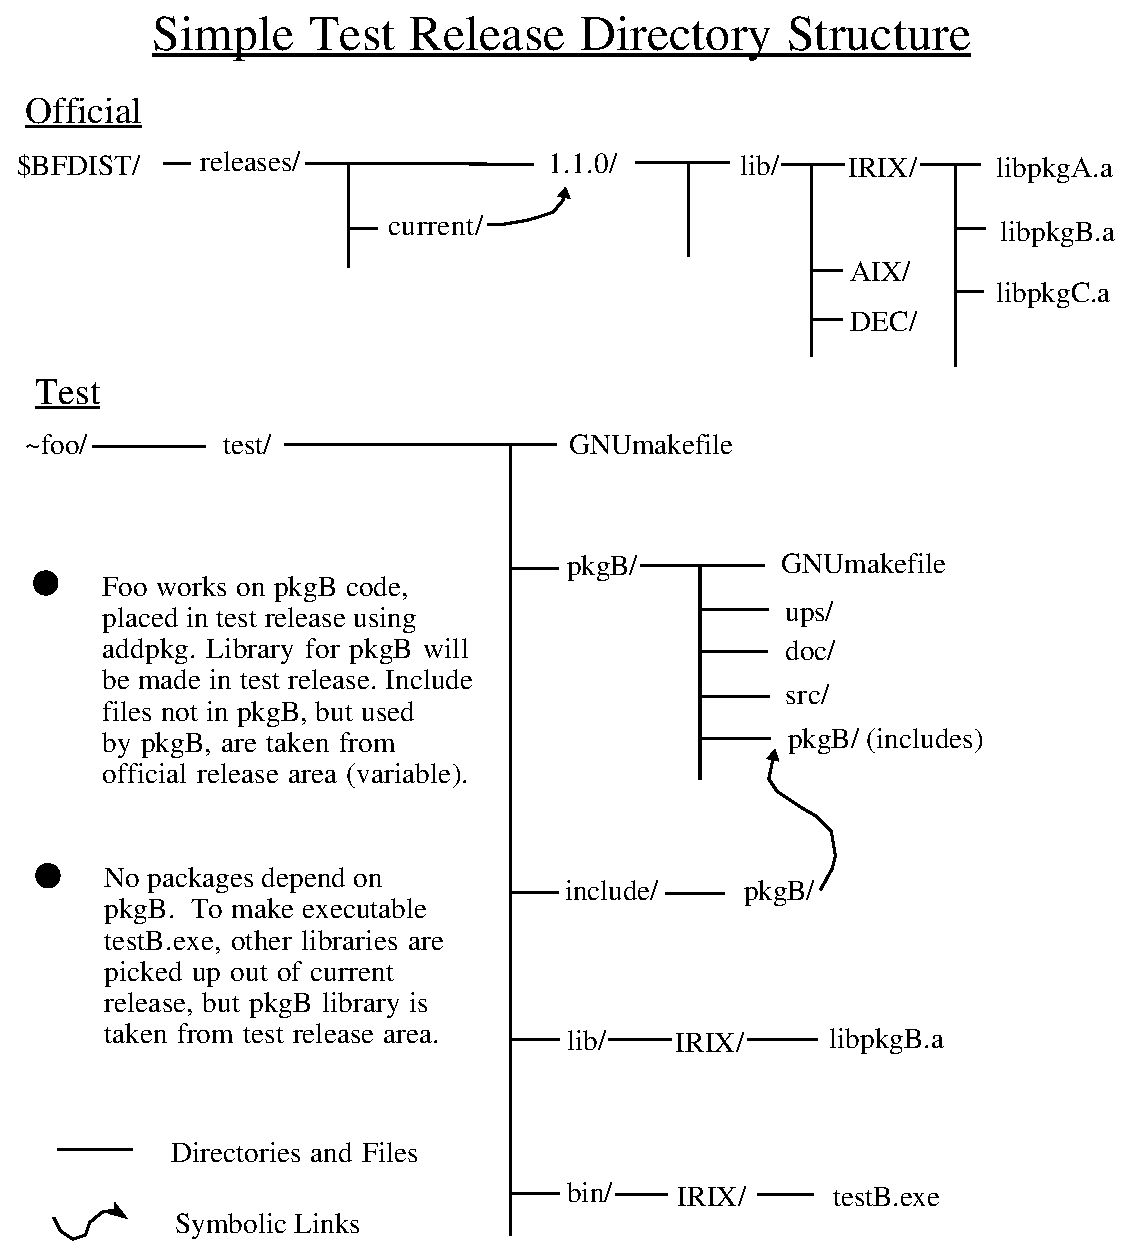
\includegraphics[width=5in]{run_2_dev_simple.eps}}
\caption[Simple Test Release Directory Structure]{ 
Diagram of a simple test release directory structure, and how it relates to the
official release directory structure.  Here the package ``pkgB'' is being
developed\index{packages!development of}, but since nothing else depends on pkgB, all other include files
\index{dependencies!simple test release} 
and libraries are taken from the current official release.}
\label{fig_dev_simple}
\end{figure}
\clearpage 

\vspace*{1.0in}
\begin{figure}[bht!]
%\epsfysize=8in
%\epsffile[36 54 581 756]{run_2_development.ps}
%\centerline{\epsfig{figure=run_2_development.eps,width=5in}}
\centerline{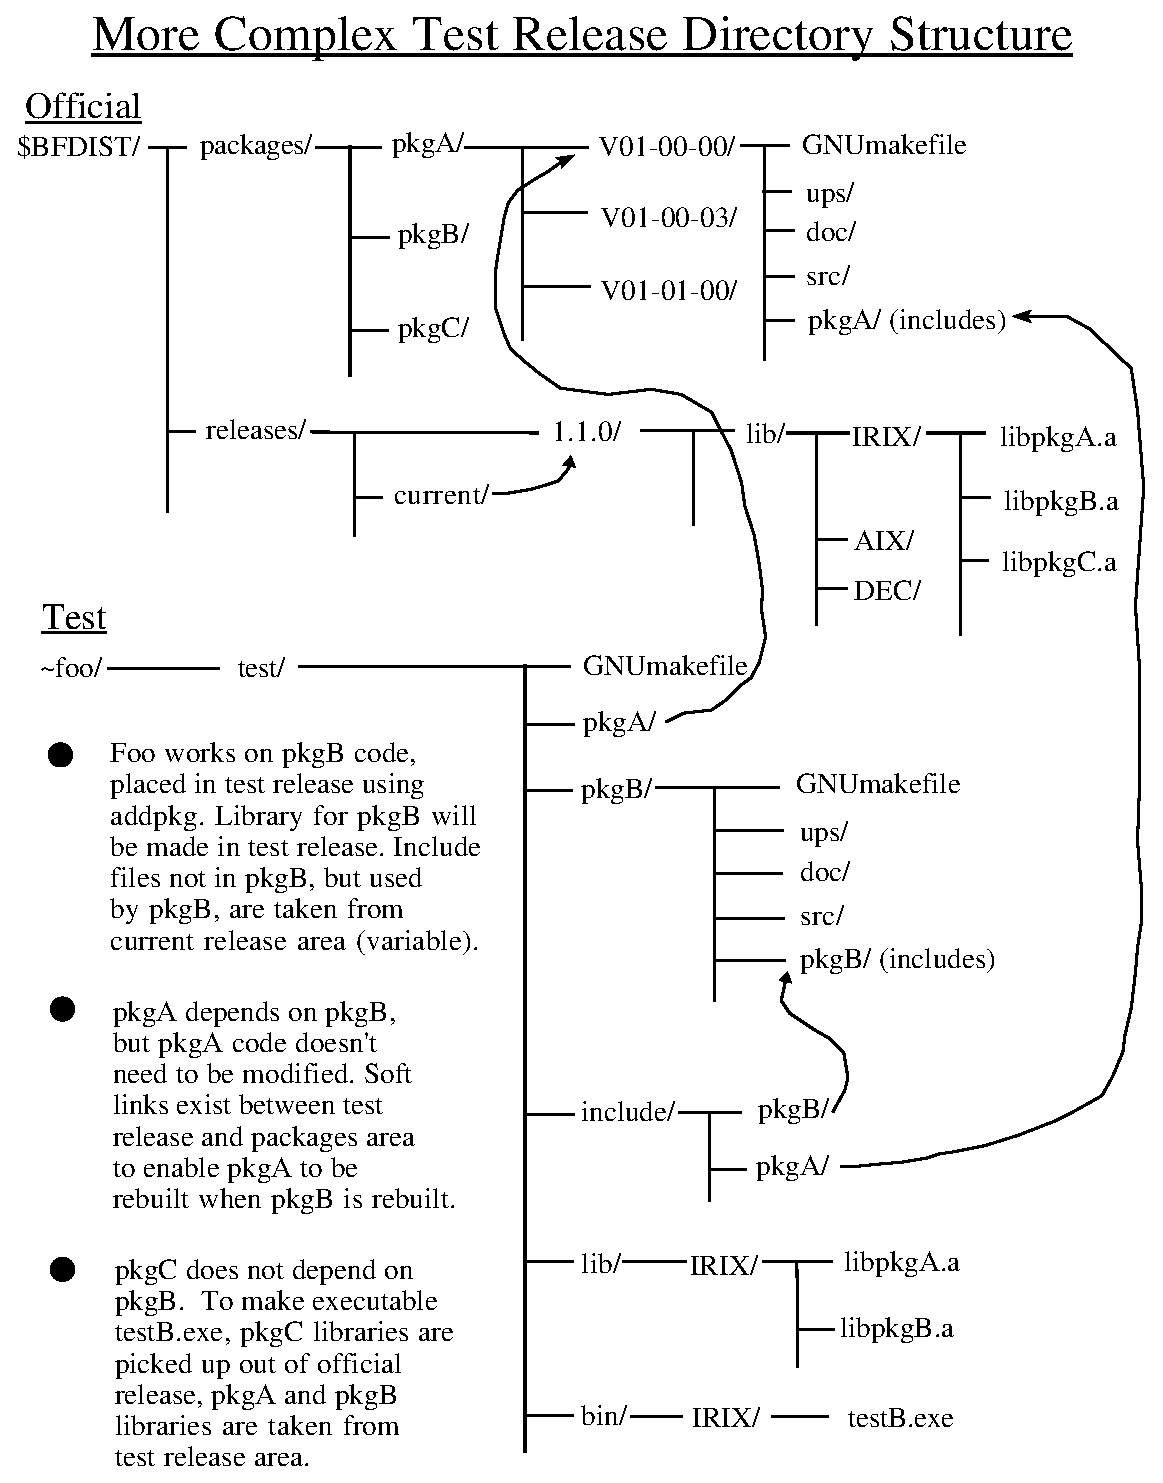
\includegraphics[width=5in]{run_2_development.eps}}
\caption[Complex Test Release Directory Structure]{ 
Diagram of a complex test release directory structure, and how it relates to the
official release directory structure.  Here the package ``pkgB'' is being
developed\index{packages!development of} , and ``pkgA'' depends on the contents of ```pkgB''. The curved lines 
\index{dependencies!complex test release} 
correspond to soft links.}
\index{soft links}
\label{fig_testrel}
\end{figure}
\clearpage 

\subsection{Distribution}
Initial distribution of the offical release structure to a remote machine will 
eventually be done via UPD once we have fully integrated it into our system.
In the meantime, we have developed simple scripts to 
initially distribute the release structure to a remote machine, 
discussed in Appendix~\ref{app_dist}.  
The release structure, those directories and soft links underneath
\index{soft links}
\$SRT\_DIST/releases in Fig.~\ref{fig_directory}, are saved in a tar file on the
server\index{client-server} machine.  
In addition, each package\index{packages!tar files}  is saved in it's own tar file. 
The location of the tarfiles on the distribution server\index{client-server} 
machines is given in ???
The
remote manager uses UPD, or currently the shell scripts described in 
Appendix~\ref{app_dist}, to copy these tar files from the distribution machine
to the remote machine and unwind them into the official 
releases\index{releases!area}  and packages\index{packages!area} 
area.  The tar file of the release specifies the flavor of the operating system and 
the version of the release. The user sets up the release using UPS as 
\index{UPS}
described in Section~\ref{sec_setup}.  The philososphy of using UPS with the
system is discussed in Appendix~\ref{app_ups}.

Once the remote machine has received an initial distribute of an official 
release, linking and development can take place. 
Distribution of the source code to a remote machine for user development is
accomplshed via SoftRelTools.  As described in section~\ref{sec_debug}, 
addpkg\index{addpkg} 
is used to checkout a complete package from CVS\index{CVS} for user development 
of that package\index{packages}. Within a test release, developers can
build and link code with their changes.  Libraries and include files from
other packages are taken from the official release. A development
release, described in section~\ref{sec_development}, can be constructed on 
any node and the code can be updated daily via CVS and rebuilt.  This is a
simple way of distributing the code to remote institutions on a daily basis,
and insuring that it works there just as well as on a central system. For
instructions on distribution of the development release at CDF, please see
section~\ref{sec_distribution_development}.

In summary, distribution of binaries and code of official 
releases\index{releases} takes place 
with UPD, after which users can link, and developers can work 
\index{linking!and distribution}
on packages  distributed to their test release by SoftRelTools.

%================================================================================
% All the appendices
%================================================================================
\input{appendix}

\clearpage
\addcontentsline{toc}{section}{References}
\begin{thebibliography}{99}

\bibitem{ref_sdss} CVS at SDSS is described on the Code Management WWW pages
at http://www-cdf.fnal.gov/offline/code\_management/sdss.html.
\index{CVS!SDSS-CVS}

\bibitem{ref_babar1} Bob Jacobsen, ``The BaBar Software Release Structure'',
\index{BaBar}
March 5, 1995, on the WWW at
http://www.slac.stanford.edu/BFROOT/dist/releases/current/SoftRelTools/ 
SoftRelToolIntro.ps.

\bibitem{ref_babar2} Bob Jacobsen, ``Using the BaBar Software Release 
Structure'', October 28, 1995, 
http://www.slac.stanford.edu/BFROOT/doc/Computing/Reconstruction/Notes/
SoftRelToolUser.ps.

\bibitem{ref_tuura} Lassi A. Tuura, ``Helper programs for Moose Directory
Structure'', http://wwwcn1.cern.ch/l/lat/www/notes/soft/dist/scripts.html.

\bibitem{ref_commentary} Walter Brown, Flavia Donno-Raffaelli and Elizabeth
Sexton-Kennedy, ``On the Software Release Directory Structure'' on the Code
Management WWW pages at 
at http://www-cdf.fnal.gov/offline/code\_management/srt.html.

\bibitem{ref_REBUILD} Flavia Donno-Raffaelli, ``REBUILD Users Guide and
Reference Manual'', CDF Note 1611, August 15, 1994.  Available on the WWW at
http://www-cdf.fnal.gov/offline/code\_management/rebuild.mem.

\bibitem{ref_cmgt_c++} See discussion of C++ implications on Code Management
\index{C++}
pages on the WWW at 
http://www-cdf.fnal.gov/offline/code\_management/c++.html.

\bibitem{ref_cvs} Basic information on cvs is available from the man pages 
and at http://fnnews.fnal.gov/cd/UNIX/cvs/cvs.html. The complete manual can
be obtained from http://www.loria.fr/$\sim$molli/cgi-bin/wilma.cgi/doc.
\index{CVS!references}.  A hardcopy of this manual is available in the CDF 
trailers office 149-E.

\bibitem{ref_cyclic} Information on Cyclic Software is available at 
http://www.cyclic.com/.

\bibitem{ref_uaf} ``UNIX at Fermilab'', Computing Division Document GU0001, 
available on the WWW at
http://www.fnal.gov/docs/UNIX/unix\_at\_fermilab/welcome.html

\bibitem{ref_alan} Alan Jonckheere, ``Configuration Management: A Turnkey 
System'', on the WWW at 
http://d0www.fnal.gov/\texttt{~}jonckheere/cmgt/turnkey.html

\bibitem{ref_dcd} Mathew Wicks, ``Fermi UNIX Environment DCD Products User
Guide'', DCD0003, DCD User Guide 3.4, January 19, 1993.

\bibitem{ref_cmgt_draft} ``Run 2 Code Management Report'', by Configuration 
Management Working Group on July 12, 1996, available on the WWW at 
http://fnpspa.fnal.gov/Run2/document.html.
\end{thebibliography}

%Index Cross References
\index{dependency files|see {.d files}} 
\index{deleting|see {removing}}
\index{get ! package|see {addpkg}}
\index{get ! test release|see {newrel}}
\index{information!about release|see {statusrel}}
\index{information!about repository|see {lscvs}}
\index{link ! symbolic|see {soft links}}
\index{link ! soft|see {soft links}}
\index{packages!installing production|see {newver}}
\index{packages!removing production|see {rmver}}
\index{packages!creating release|see {newrel}}
\index{packages!interdependencies|see {depend}}
\index{packages!soft links|see {lnkpkg}}
\index{packages!getting|see {addpkg}}
\index{packages!removing release|see {rmrel}}
\index{release!listing contents|see {statusrel}}
\index{release!creating|see {newrel}}
\index{release!removing see {rmrel}}
\index{removing!releases|see {rmrel}}
\index{removing!packages|see {rmver}}
\index{new ! production package|see {newver}}
\index{soft links!creating|see {lnkpkg}}
\index{compile!UPS |see {UPS}}
\index{UPS!dependencies|see {dependencies|UPS}}
\index{server|see {client-server}}
\index{linking!executable filename|see {EXENAME}}
\index{linking!.opt filename|see {OPTFILE}}
\index{make|see {gmake}}
\index{preprocessor|see {CPP}}
\index{version!control|see {CVS}}

\clearpage
\addcontentsline{toc}{section}{Index}
\input{run2_cmgt.ind}
\end{document}

\end{document}

\end{document}

\end{document}
